% This text is proprietary.
% It's a part of presentation made by myself.
% It may not used commercial.
% The noncommercial use such as private and study is free
% Dec 2007
% Author: Sascha Frank
% University Freiburg
% www.informatik.uni-freiburg.de/~frank/
%
%
\documentclass{beamer}
%\documentclass[12pt]{article}
%\usepackage{beamerarticle}

\usepackage[utf8]{inputenc}

%This part is to get four quadrants in the minipage
\usepackage{caption}
\newcommand\FourQuad[4]{%
    \begin{minipage}[b][.35\textheight][t]{.47\textwidth}#1\end{minipage}\hfill%
    \begin{minipage}[b][.35\textheight][t]{.47\textwidth}#2\end{minipage}\\[0.5em]
    \begin{minipage}[b][.35\textheight][t]{.47\textwidth}#3\end{minipage}\hfill
    \begin{minipage}[b][.35\textheight][t]{.47\textwidth}#4\end{minipage}%
}
\setbeamertemplate{navigation symbols}{}

\usepackage{animate}
\usepackage{amsmath}
%\usepackage[landscape]{geometry}
%\usepackage{tikz}
%\usetikzlibrary{mindmap}
%\usepackage{metalogo}
%\usepackage{dtklogos}

\usetheme{Warsaw} \usepackage{color} \usepackage{chemmacros}
\usepackage{verbatim}

\setbeamercovered{invisible}
\beamersetuncovermixins{\opaqueness<1>{25}}{\opaqueness<2->{15}}
\begin{document}
% logo of my university
%\titlegraphic{\vspace*{-5cm} \hspace*{8.75cm} 
\includegraphics[width=1.5cm]{umea_logo.eps}
%}
%\logo{
\includegraphics[width=1.5cm]{umea_logo.eps}
%}

\title{Computational Chemistry - MD Simulations} \author{P. Ojeda-May \\{\small pedro.ojeda-may@umu.se}} 
\institute[Ume\aa~ University]{Department of Chemistry/HPC2N, \\
Ume\aa~ University,\\[1em]
\includegraphics[width=0.8cm]{../umea_logo.eps} \\
901 87, Sweden.}

\date{\today}


%%%%%%%%%%%%%%%%% NEW  SLDE
\begin{frame}
\titlepage
\end{frame}

%%%%%%%%%%%%%%%%% NEW  SLDE
\begin{frame}\frametitle{Table of contents}\tableofcontents \end{frame}

%%%%%%%%%%%%%%%%% NEW  SLDE
%\begin{frame}\frametitle{Background }
%
%\begin{figure}
%\includegraphics[scale=0.2]{../map.eps}
%%\caption{{\scriptsize Background.  }}
%\end{figure}
%
%\end{frame}

%%%%%%%%%%%%%%%%%% NEW  SLDE
%\begin{frame}\frametitle{Background  }
%
%\begin{itemize}
%\item<1-> Physicist currently working on Chemistry.
%
%\item<2-> Experience with Supercomputers and HPC Clusters. 
%
%\item<3-> Code developer of Chemistry at Harvard Molecular Mechanics (CHARMM) package:  
%
%	\begin{itemize}
%		\item Carr-Parrinello Molecular Dynamics
%		\item Multiple time steps algorithms
%		\item Modified Neglect of Diatomic Overlap (MNDO) QM/MM approach
%		\item Hybrid MPI/OpenMP approches for QM/MM simulations
%		\item QM/MM-Cutoff methods.
%	\end{itemize}
%\end{itemize}
%
%
%\end{frame}


\section{Basics on MD simulations }
\subsection{Force field} 


%%%%%%%%%%%%%%%%% NEW  SLDE
\begin{frame}\frametitle{Simulations time scale}

\begin{figure}
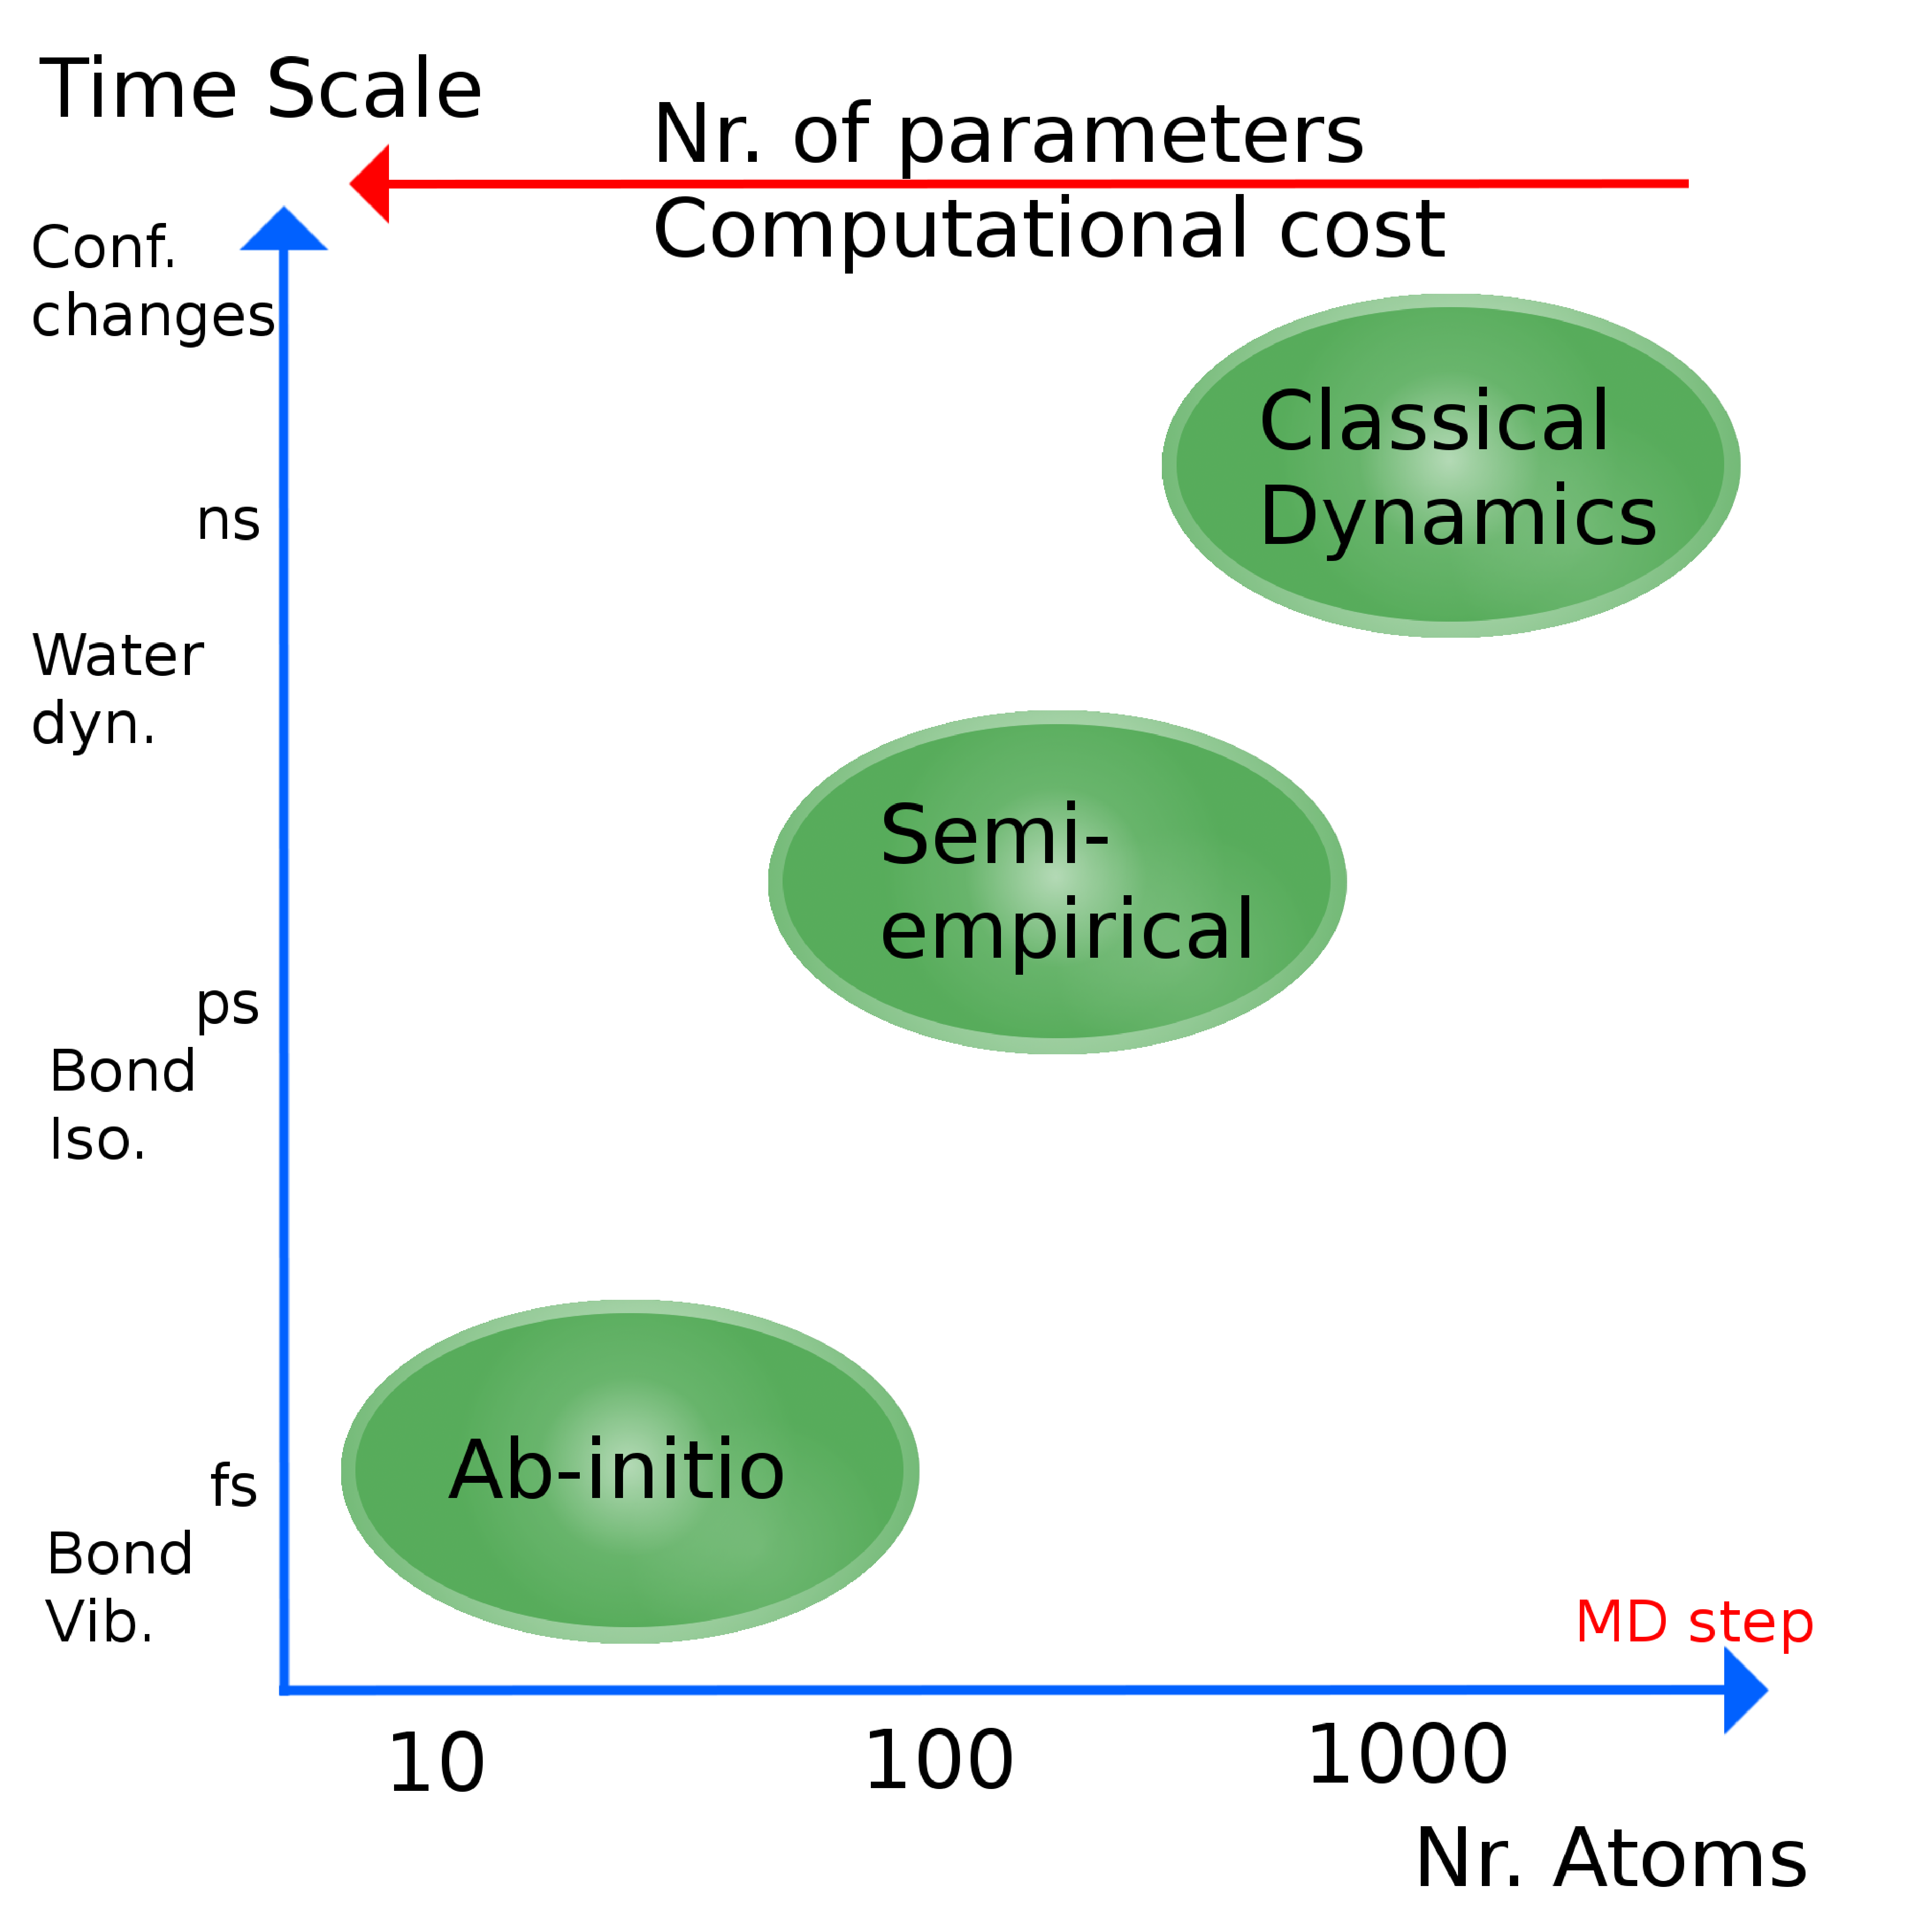
\includegraphics[scale=0.081]{../simul_time_scales.eps}
\caption{{\scriptsize Accuracy w.r.t. time scale for different modeling approaches.}}
\end{figure}

\end{frame}

%%%%%%%%%%%%%%%%% NEW  SLDE
\begin{frame}\frametitle{Early MD simulations}

\begin{minipage}[t]{0.4\linewidth}

\begin{figure}
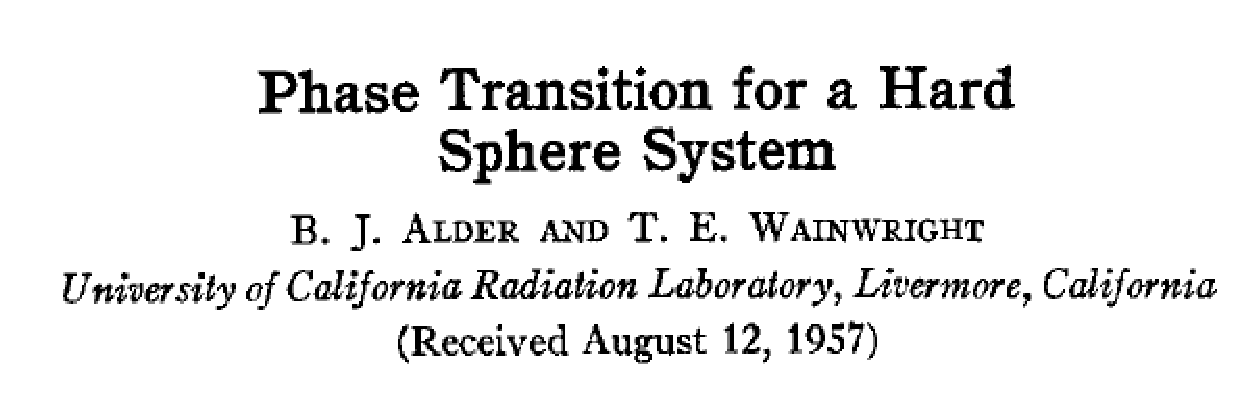
\includegraphics[scale=0.16]{hard_spheres.eps}
%\caption{{\scriptsize  AdK enzyme in water.}}
\end{figure}

\end{minipage}
%}%
\hfill%
%\fbox{%
\begin{minipage}[t]{0.58\linewidth}
\begin{figure}
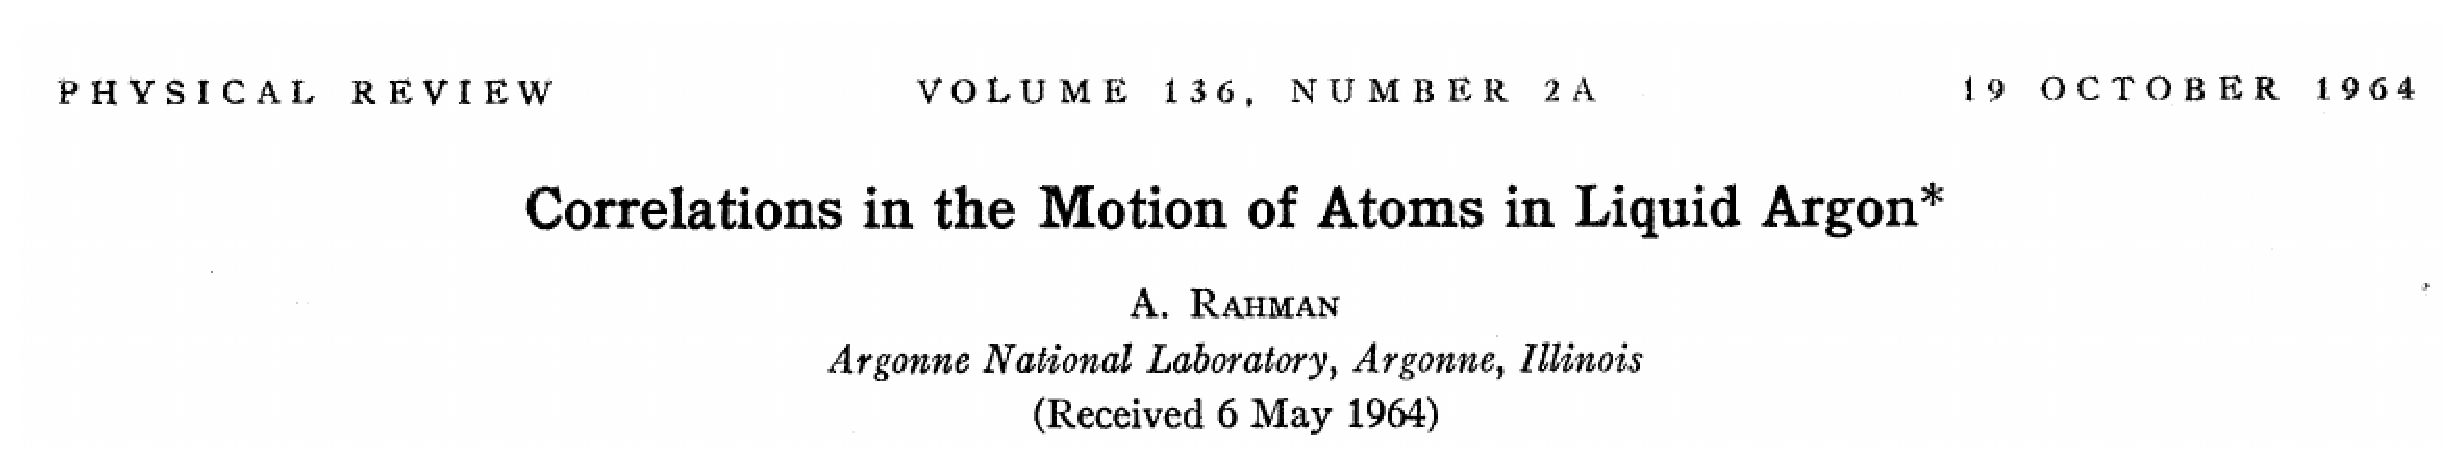
\includegraphics[scale=0.21]{rahman_1964.eps}
%\caption{{\scriptsize  Clay [JPC C, {\bf 118}, 1001 (2014)].}}
\end{figure}
\end{minipage}

\begin{figure}
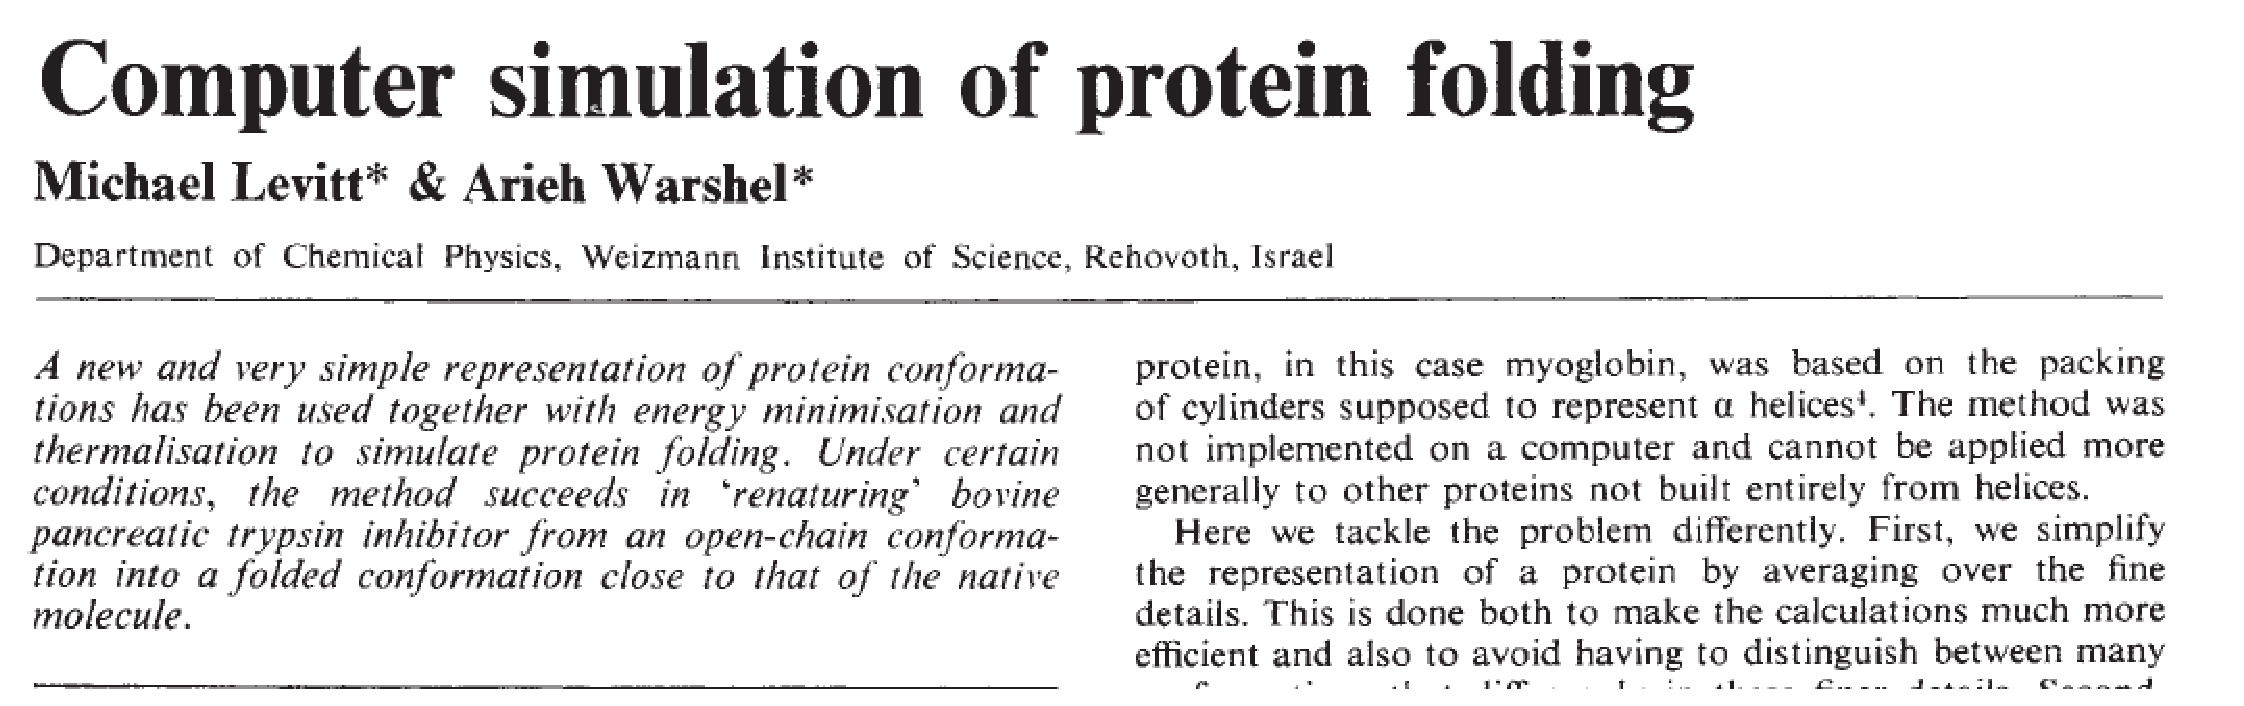
\includegraphics[scale=0.19]{levitt_1975.eps}
\caption{{\scriptsize Nature, {\bf 253} (1975).}}
\end{figure}

\end{frame}

%%%%%%%%%%%%%%%%% NEW  SLDE
\begin{frame}\frametitle{Current MD simulations}

\begin{figure}
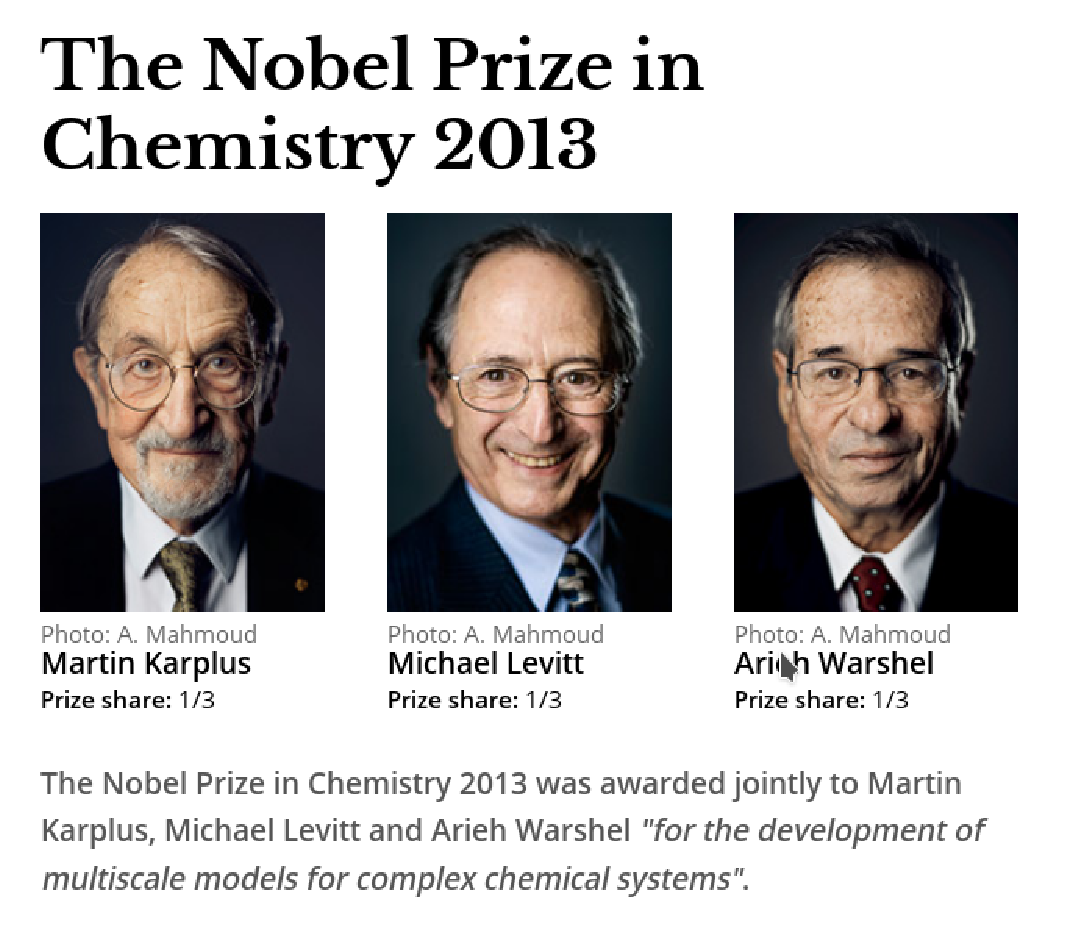
\includegraphics[scale=0.33]{nobel_prize.eps}
\caption{{\scriptsize Source: http://www.nobelprize.org.}}
\end{figure}

\end{frame}



%%%%%%%%%%%%%%%%% NEW  SLDE
\begin{frame}\frametitle{Current MD simulations}

\begin{figure}
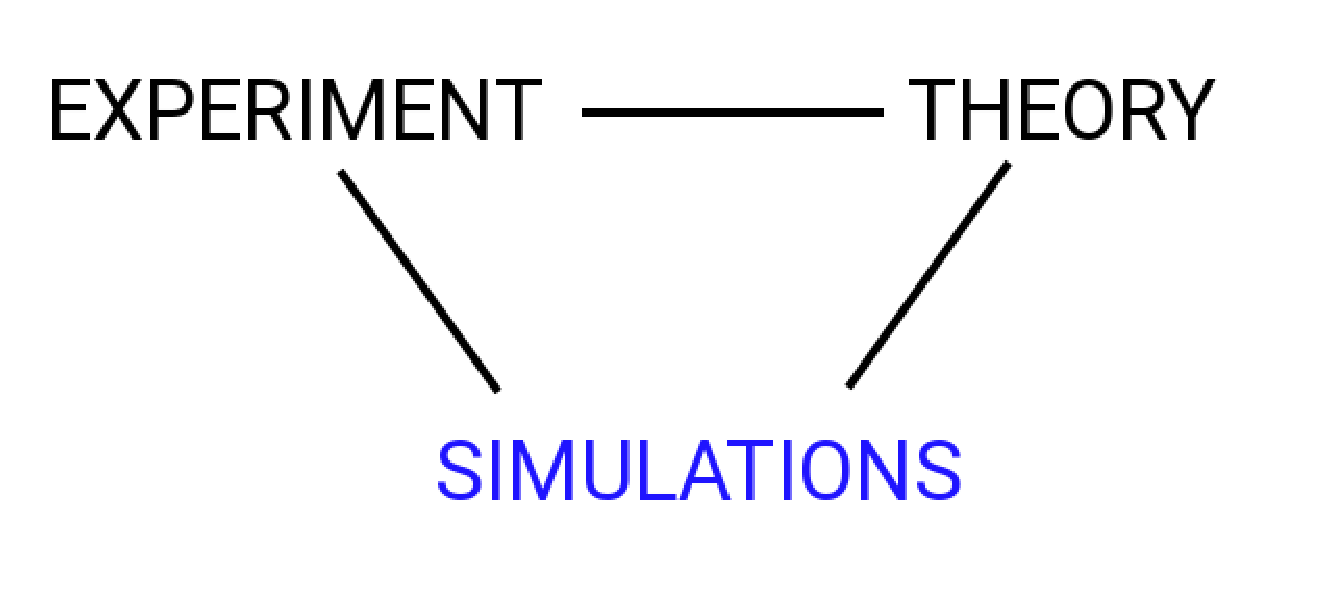
\includegraphics[scale=0.39]{three_approaches.eps}
%\caption{{\scriptsize Source: http://www.nobelprize.org.}}
\end{figure}

\end{frame}




%%%%%%%%%%%%%%%%% NEW  SLDE
\begin{frame}
  \frametitle{Application of MD}

\begin{minipage}[t]{0.48\linewidth}

Proteins
\begin{figure}
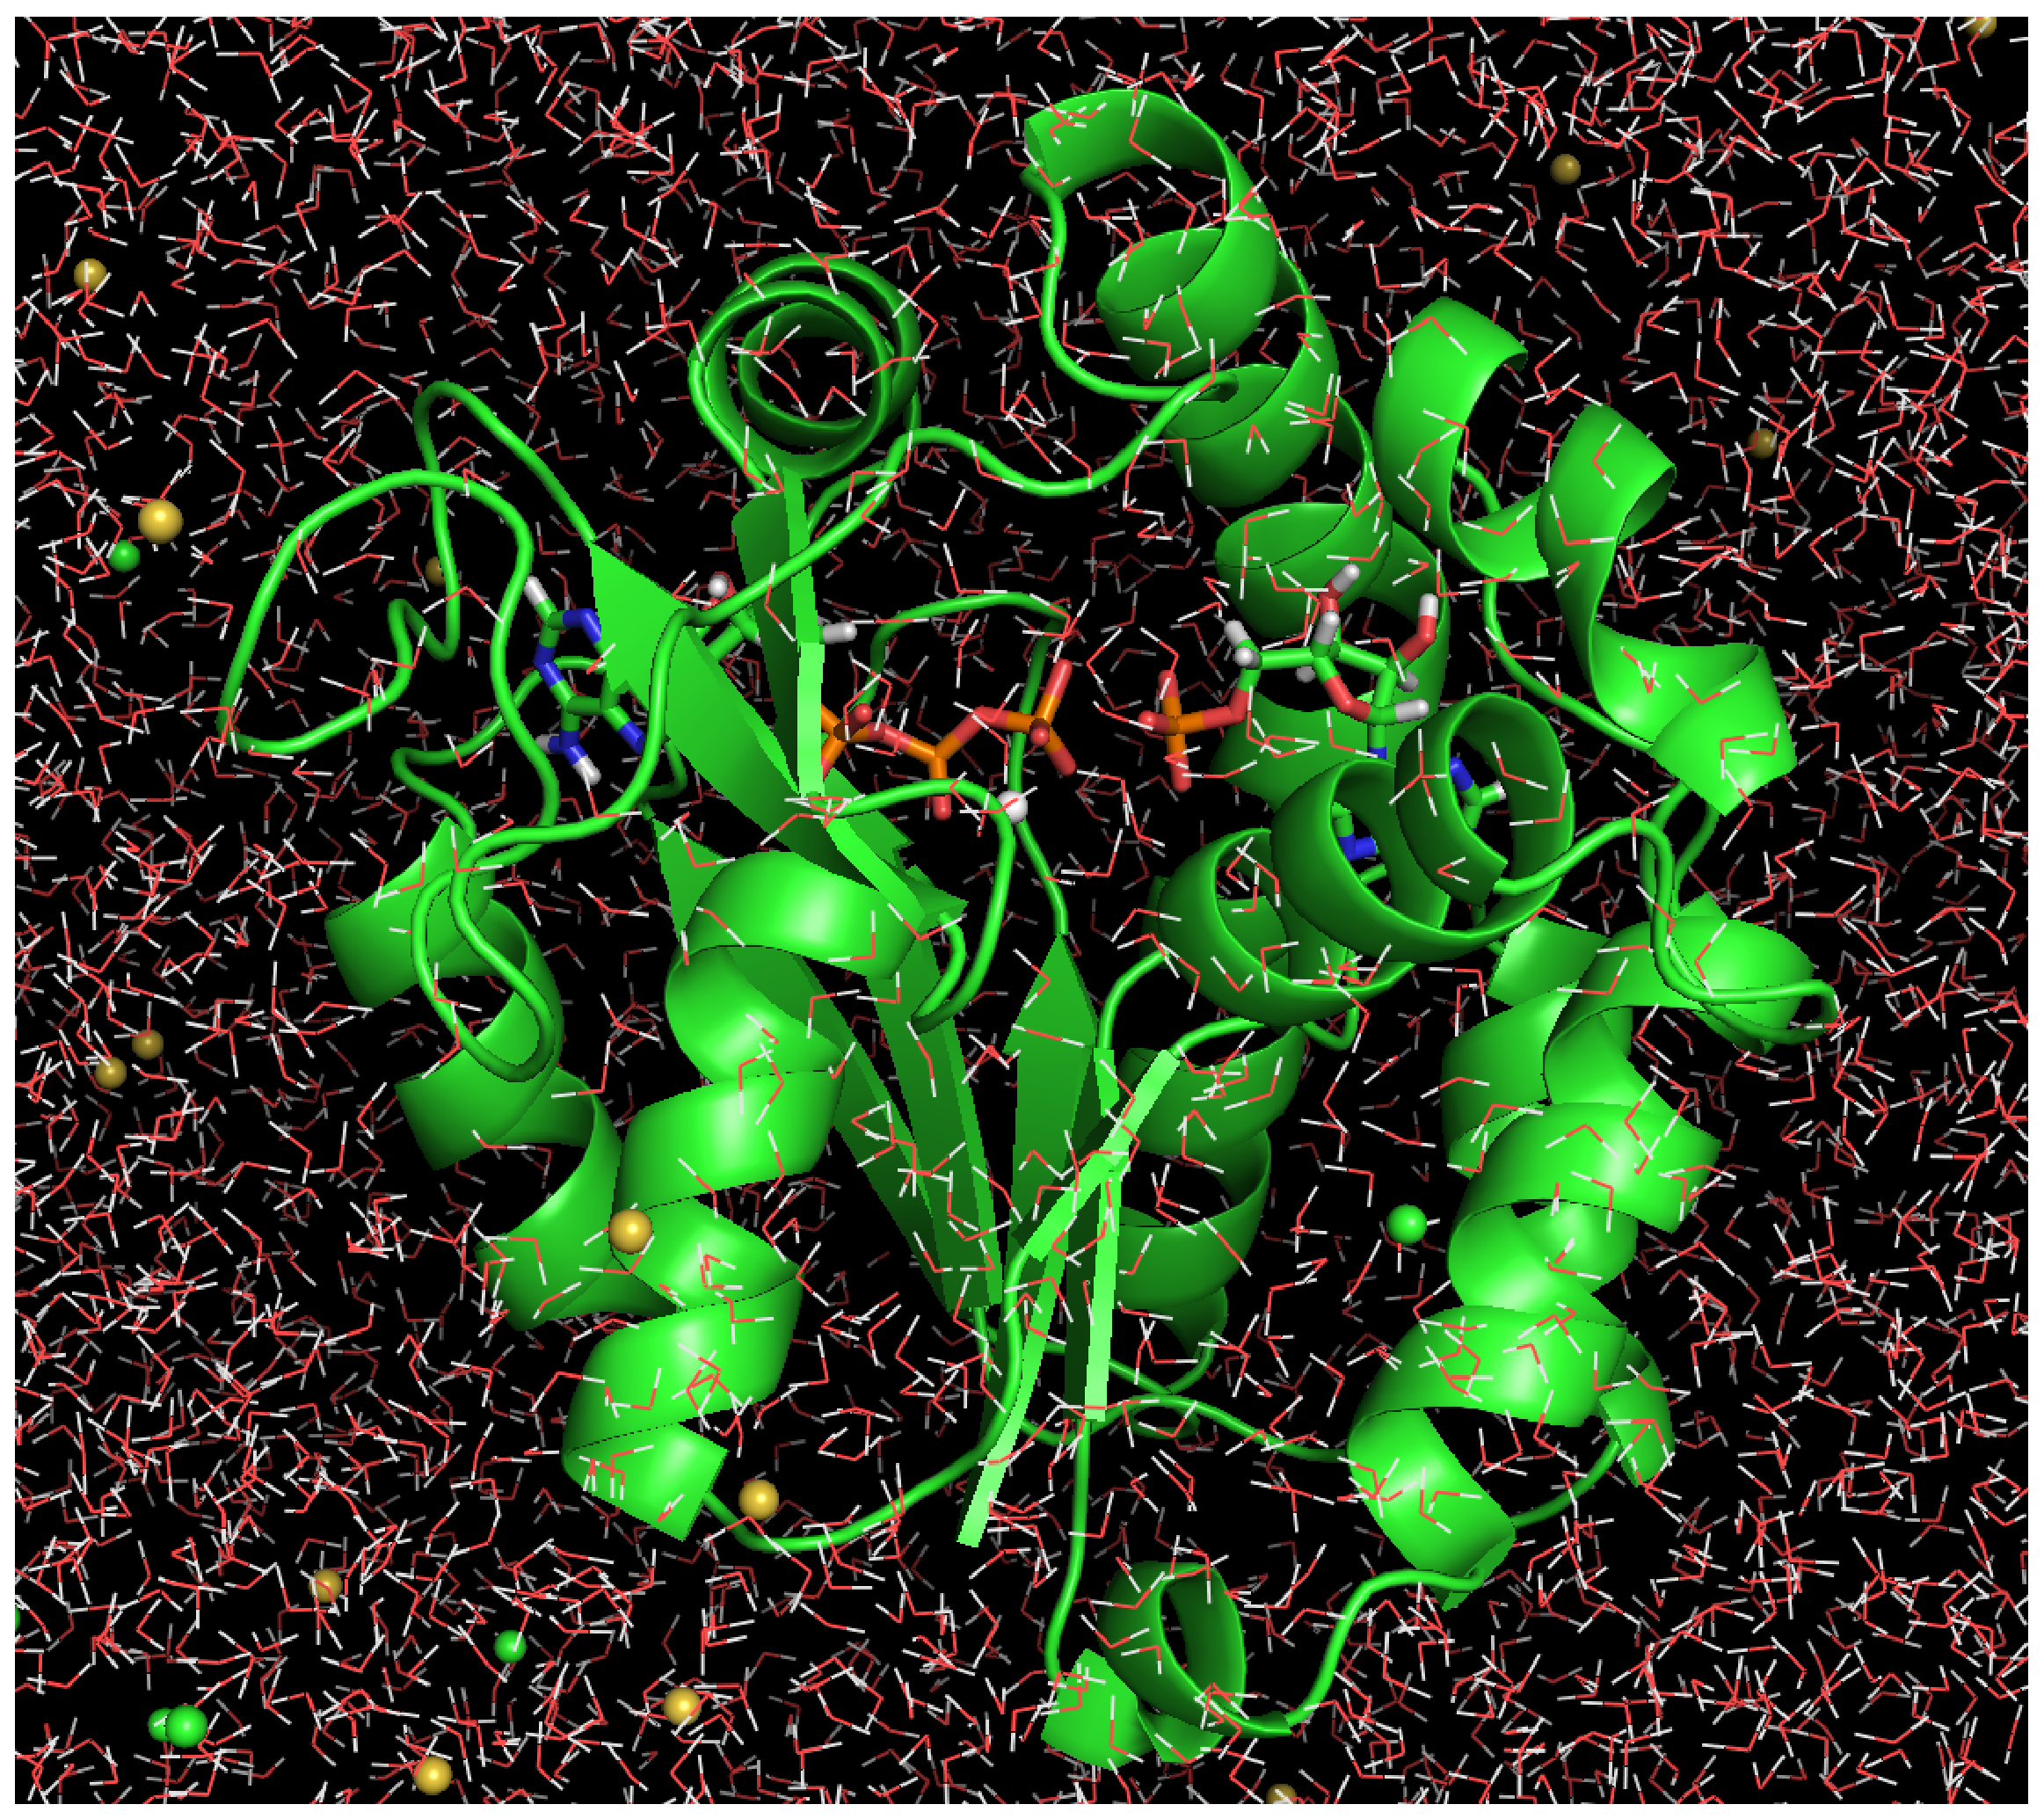
\includegraphics[scale=0.135]{../protein_water_ligand_ions.eps}
\caption{{\scriptsize  AdK enzyme in water.}}
\end{figure}

\end{minipage}
%}%
\hfill%
%\fbox{%
\begin{minipage}[t]{0.48\linewidth}
Clays
\begin{figure}
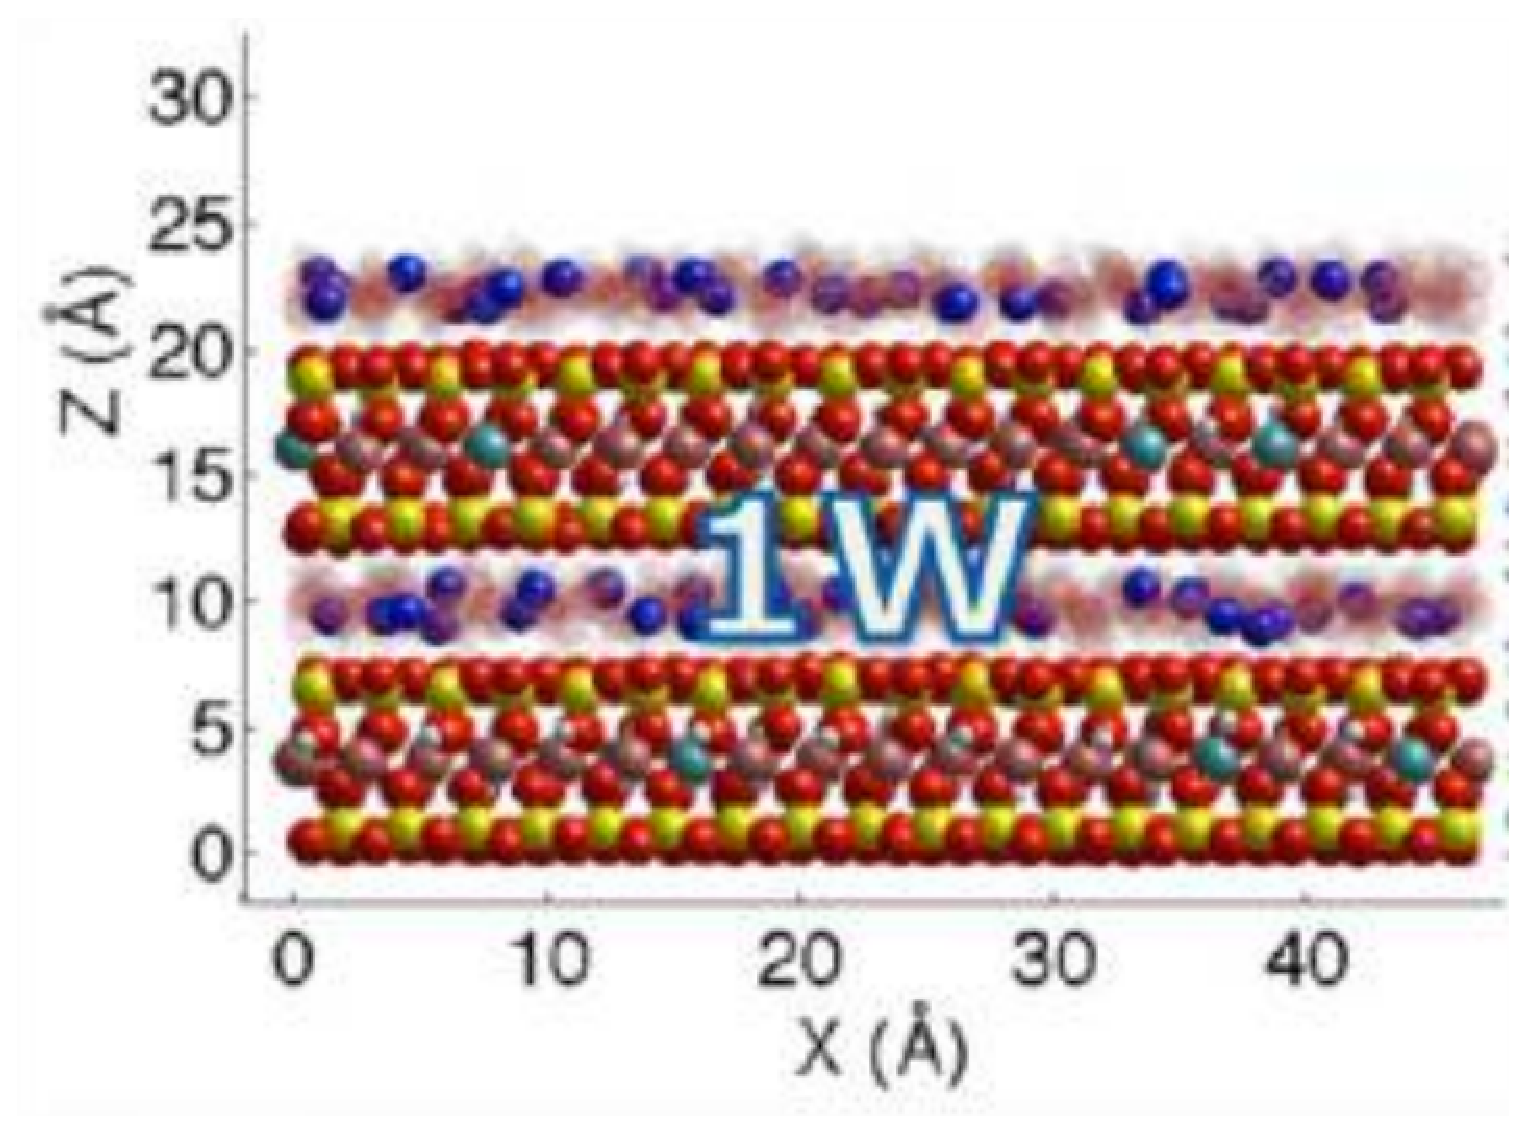
\includegraphics[scale=0.2]{clay.eps}
\caption{{\scriptsize  Clay [JPC C, {\bf 118}, 1001 (2014)].}}

\end{figure}
\end{minipage}
\end{frame}

%%%%%%%%%%%%%%%%% NEW  SLDE
\begin{frame}
  \frametitle{Application of MD}


\begin{figure}

\includegraphics[scale=0.2]{icecream.eps}
\caption{{\scriptsize  Ice cream research.}}
\end{figure}

\end{frame}

%%%%%%%%%%%%%%%%% NEW  SLDE
\begin{frame}
  \frametitle{Application of MD}

\begin{minipage}[t]{0.48\linewidth}

\begin{figure}

\includegraphics[scale=0.17]{asphalt.eps}
\caption{{\scriptsize  Asphalt research.}}
\end{figure}

\end{minipage}
%}%
\hfill%
%\fbox{%
\begin{minipage}[t]{0.48\linewidth}
\begin{figure}
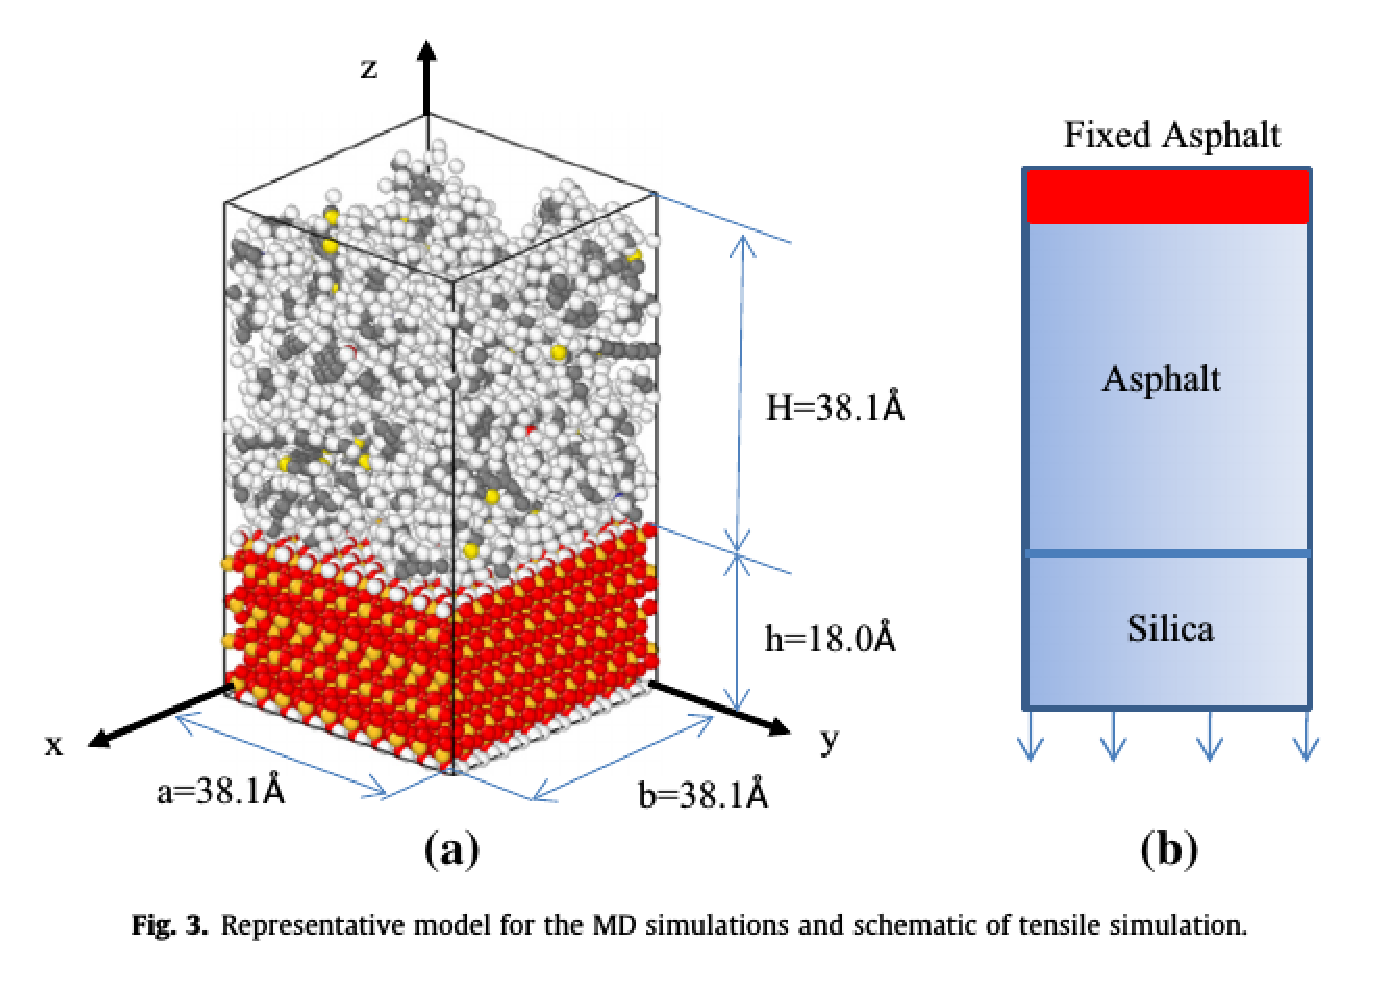
\includegraphics[scale=0.25]{asphalt2.eps}
\caption{{\scriptsize  Asphalt [Const. Build. Mat., {\bf 121}, 246 (2016)].}}
\end{figure}
\end{minipage}
\end{frame}

%%%%%%%%%%%%%%%%% NEW  SLDE

\begin{frame}
  \frametitle{Newton's equation}
  
  \begin{equation}
	  \mathbf{F}= - \mathbf{\nabla} U      \mathrm{~~~~~~~~~~Newton's~ Law (1687)}
  \end{equation}

  solution of this equation requires the knowledge of an array of
  particles' positions and velocities

  \begin{equation}
          \mathbf{X}= (x^1_1,x^1_2,x^1_3 ~,~ x^2_1,x^2_2,x^2_3 ~\ldots~ x^N_1,x^N_2,x^N_3~)
  \end{equation}


  \begin{equation}
          \mathbf{V}= (v^1_1,v^1_2,v^1_3~,~ v^2_1,v^2_2,v^2_3 ~\ldots~ v^N_1,v^N_2,v^N_3~)
  \end{equation}

\end{frame}


%%%%%%%%%%%%%%%%% NEW  SLDE
\begin{frame}\frametitle{Force fields}

\begin{figure}
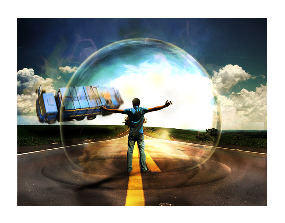
\includegraphics[scale=1.481]{force_field_squarespace.eps}
\caption{{\scriptsize Source: http://www.lpwchem.org/force-field-development/}}
\end{figure}

\end{frame}

%%%%%%%%%%%%%%%%% NEW  SLDE
\begin{frame}\frametitle{Force fields}

\begin{equation}
\begin{aligned}
	U  = & \sum_{\textrm{bonds}} \frac{1}{2} k_{\textrm{bonds}} (r-r_0)^2 + \sum_{\textrm{angles}} \frac{1}{2} k_{\textrm{angle}} 
	(\theta-\theta_0)^2 \\
	&+\sum_{\textrm{torsions}} \sum_j V_j(1+\textrm{cos}j\phi)  \\
 &+ \sum_{\textrm{Coulomb}}^{i<j} \frac{q_i q_j}{r_{ij}}  +  \sum_{\textrm{VdW}}^{i<j} 
\left\{ 4\epsilon_{ij} \left[ \left( \frac{\sigma_{ij}}{r_{ij}} \right)^{12}-  \left( \frac{\sigma_{ij}}{r_{ij}} \right)^{6} \right]  \right\}
\end{aligned}
\end{equation}


\end{frame}

%%%%%%%%%%%%%%%%% NEW  SLDE
\begin{frame}\frametitle{Force fields}

\begin{figure}
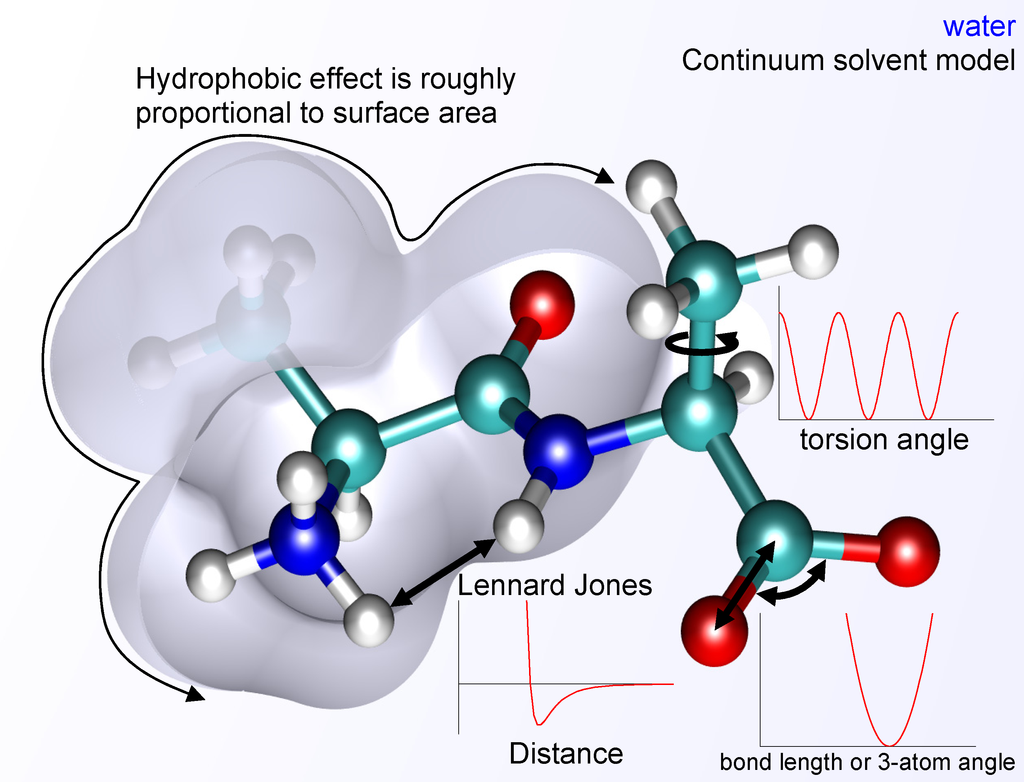
\includegraphics[scale=1.441]{1024px-MM_PEF.png}
\caption{{\scriptsize Energy terms. Source: https://en.wikipedia.org/wiki/Force\_field\_(chemistry)}}
\end{figure}


\end{frame}

%%%%%%%%%%%%%%%%% NEW  SLDE
\begin{frame}\frametitle{Force fields}

\begin{figure}
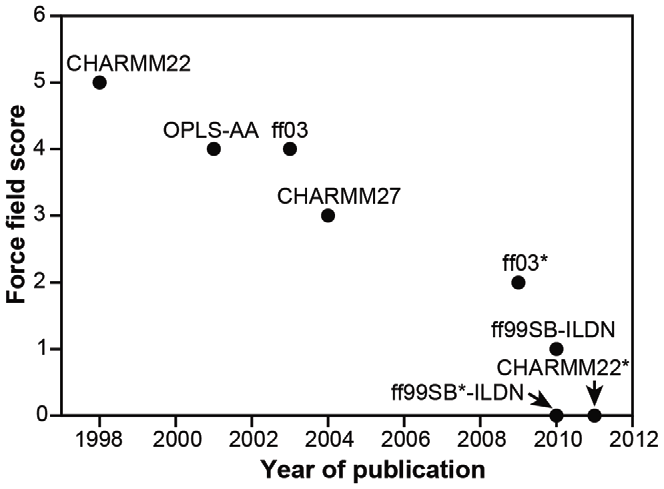
\includegraphics[scale=0.34]{ff_comparison.png}
\caption{{\scriptsize FF for proteins comparison, PLoS ONE, 7, e32131, (2012).}}
\end{figure}


\end{frame}

%%%%%%%%%%%%%%%%% NEW  SLDE
\begin{frame}\frametitle{Force fields: Energy surface}

\begin{figure}
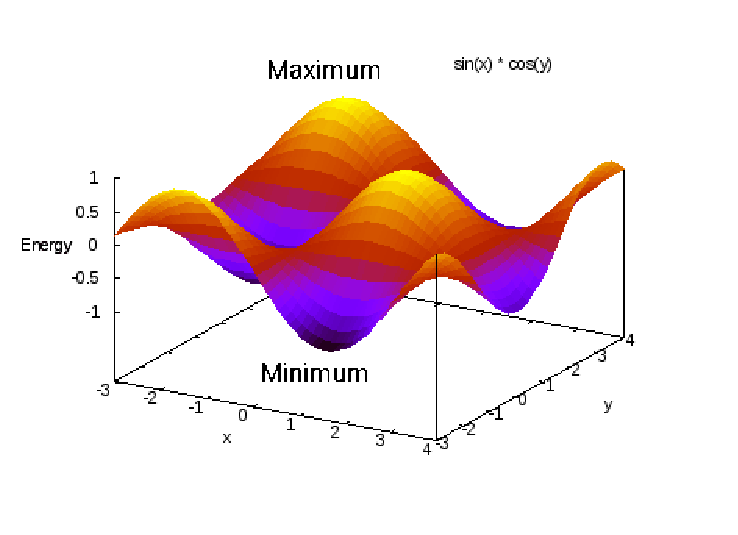
\includegraphics[scale=0.681]{surface.eps}
\caption{{\scriptsize Energy surface described by $U=sin(x)*cos(x)$}}
\end{figure}

\end{frame}

%%%%%%%%%%%%%%%%% NEW  SLDE
\begin{frame}\frametitle{Force fields}

\begin{itemize}
\item Proteins and Hydrocarbons: GROMOS, OPLS-AA, AMBER, CHARMM.
\item Clays: CLAYFF
\item Coarse-graining: MARTINI
\end{itemize}

If the parameters of your compound are not part of the force field you need to use QM approaches.

\end{frame}

%%%%%%%%%%%%%%%%% NEW  SLDE
\begin{frame}\frametitle{Water models}

\begin{figure}
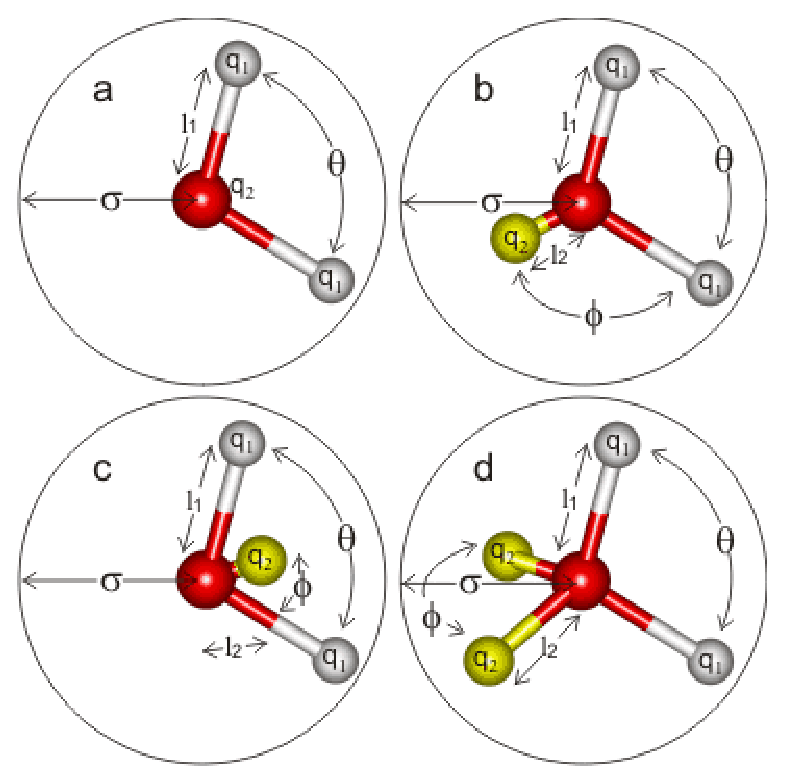
\includegraphics[scale=0.34]{h2o_models.eps}
\caption{{\scriptsize 3-5 sites water models. Source: http://www1.lsbu.ac.uk/water/water\_models.html}}
\end{figure}

\end{frame}


%%%%%%%%%%%%%%%%% NEW  SLDE
\begin{frame}\frametitle{Water models}

\begin{figure}
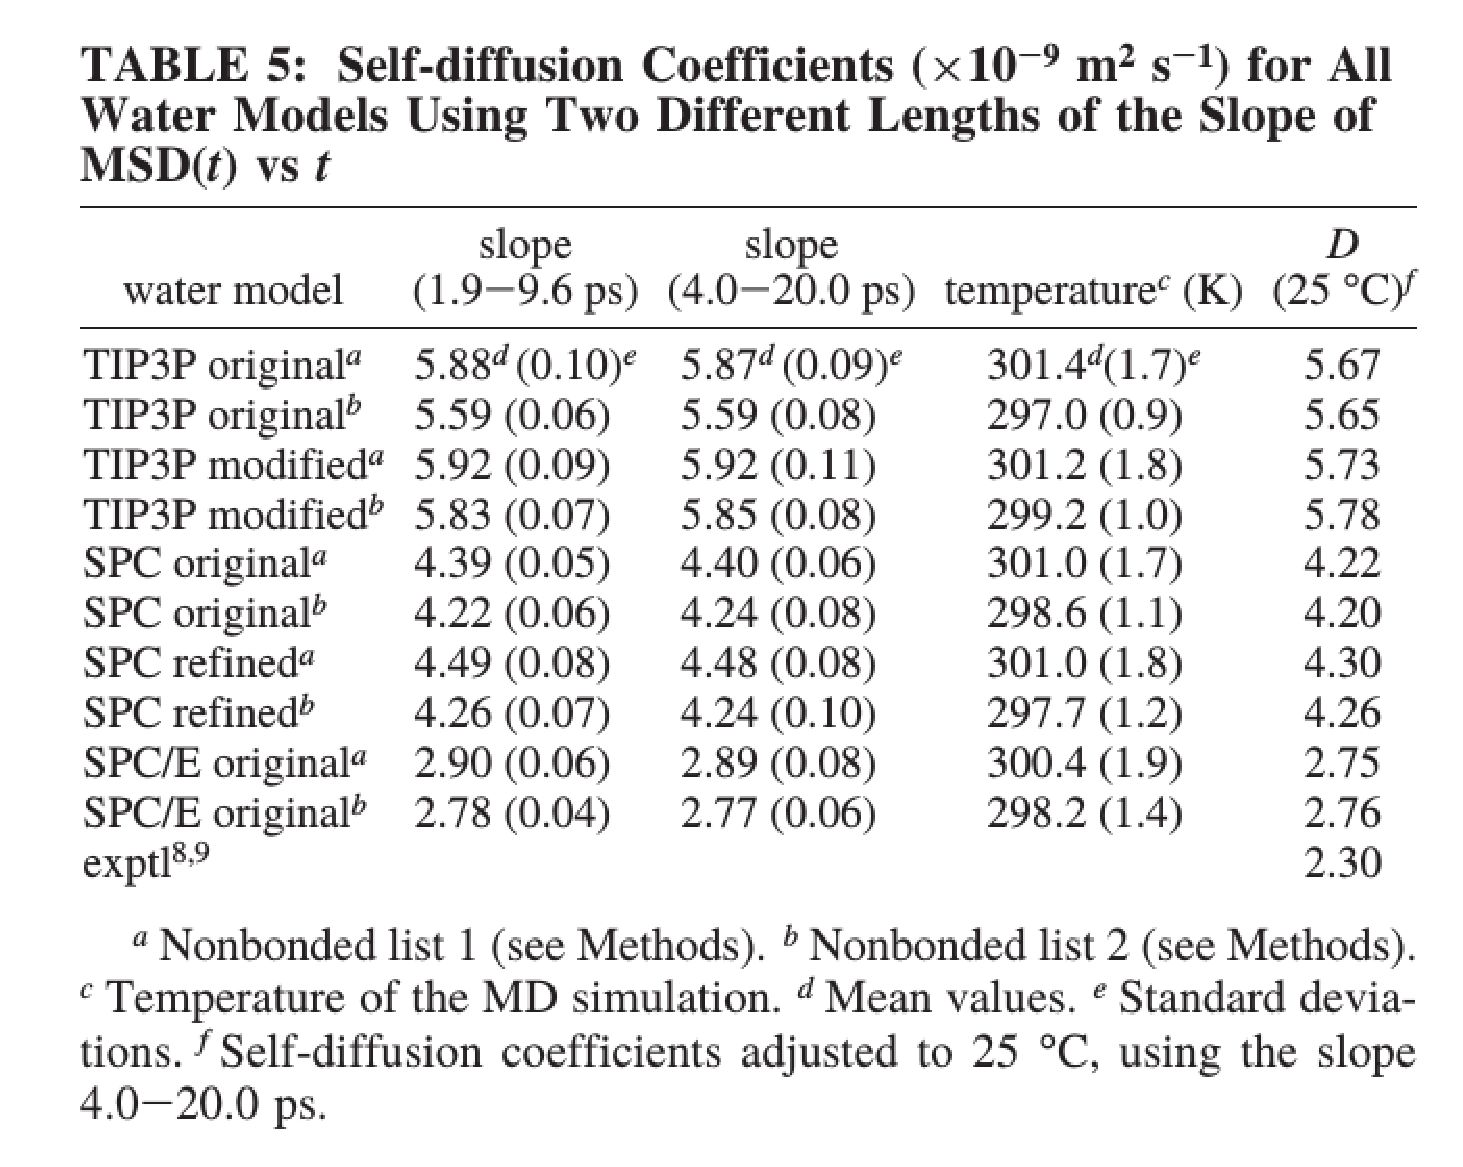
\includegraphics[scale=0.3]{nilsson_water.eps}
\caption{{\scriptsize See for details: JPC A, {\bf 105}, 9954 (2001). }}
\end{figure}

\end{frame}


%%%%%%%%%%%%%%%%% NEW  SLDE
\begin{frame}\frametitle{Protein systems}

\begin{figure}
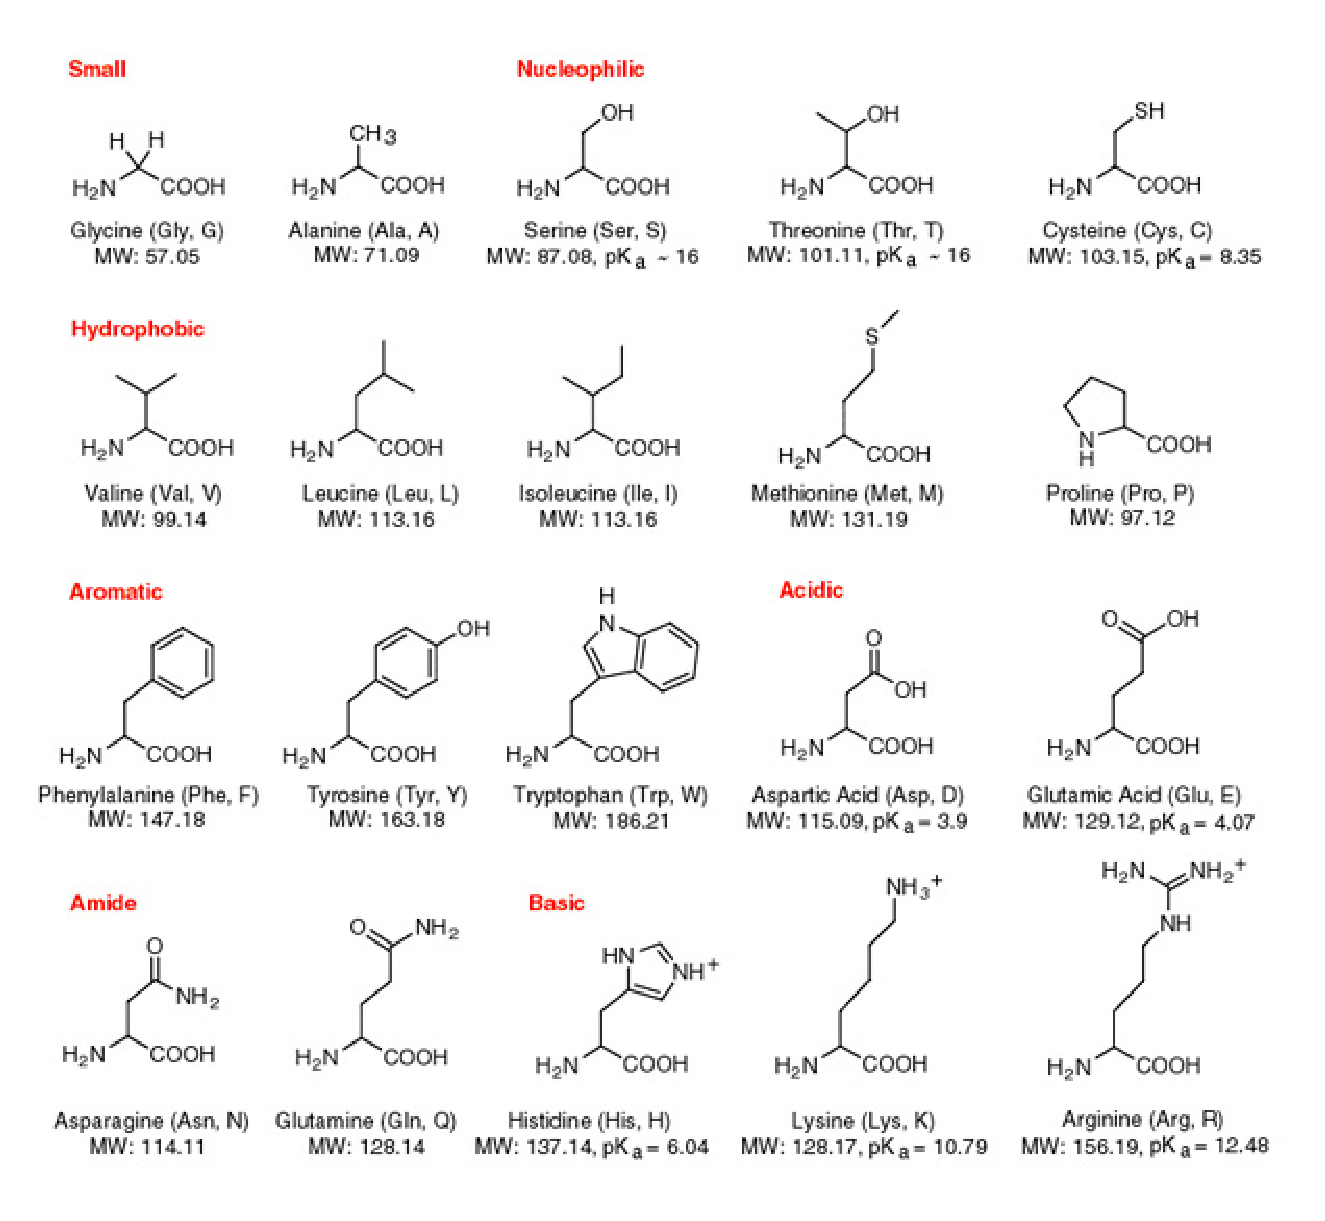
\includegraphics[scale=0.3]{aminoacids.eps}
\caption{{\scriptsize 20 natural amino acids. Source: goo.gl/YrYvwv}}
\end{figure}

\end{frame}

%%%%%%%%%%%%%%%%% NEW  SLDE
\begin{frame}\frametitle{Protein systems}


\begin{minipage}[t]{0.48\linewidth}

\begin{figure}
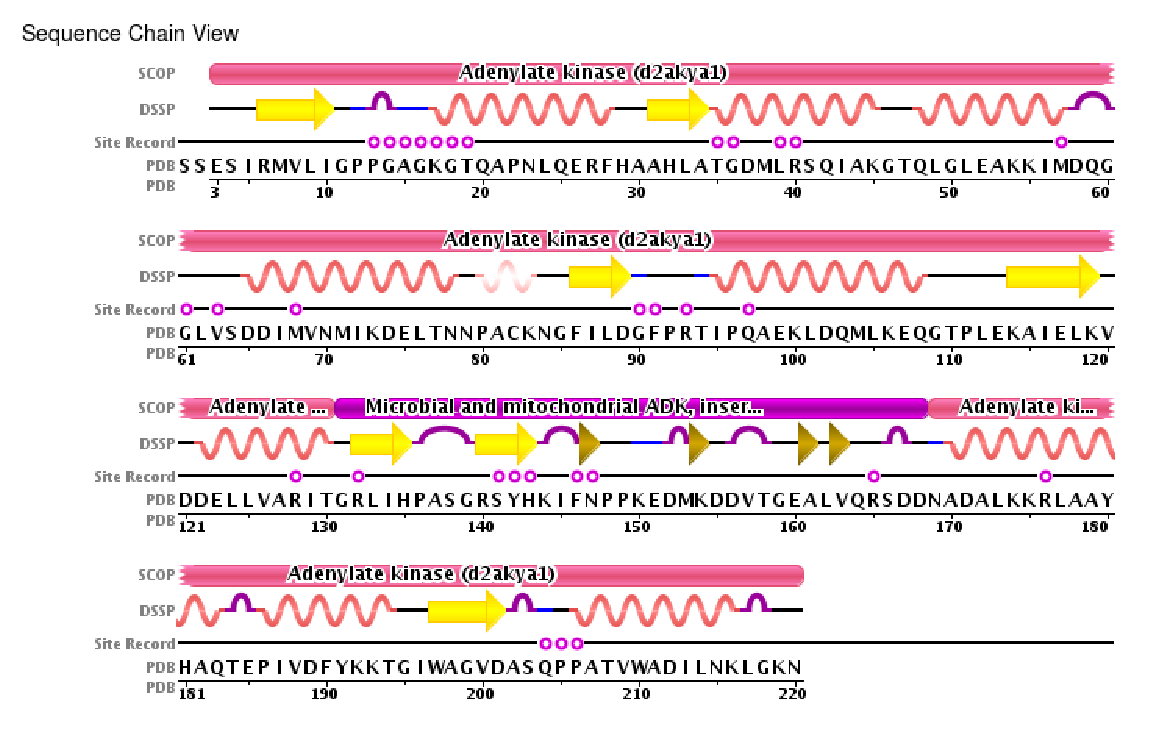
\includegraphics[scale=0.31]{pdb_2aky.eps}
\caption{{\scriptsize PDB information of AdK.}}
\end{figure}
 
\end{minipage}
\hfill%
\begin{minipage}[t]{0.48\linewidth}
\begin{figure}
\includegraphics[scale=0.36]{2aky_domains.eps}
\caption{{\scriptsize Structure of yeast AdK.}}
\end{figure}
\end{minipage}

\end{frame}


%%%%%%%%%%%%%%%%% NEW  SLDE
\begin{frame}\frametitle{Periodic boundary conditions (PBC)}
The systems we can study with MD simulations are tiny compared to real experimental setups ($10^{23} particles$).

\begin{figure}
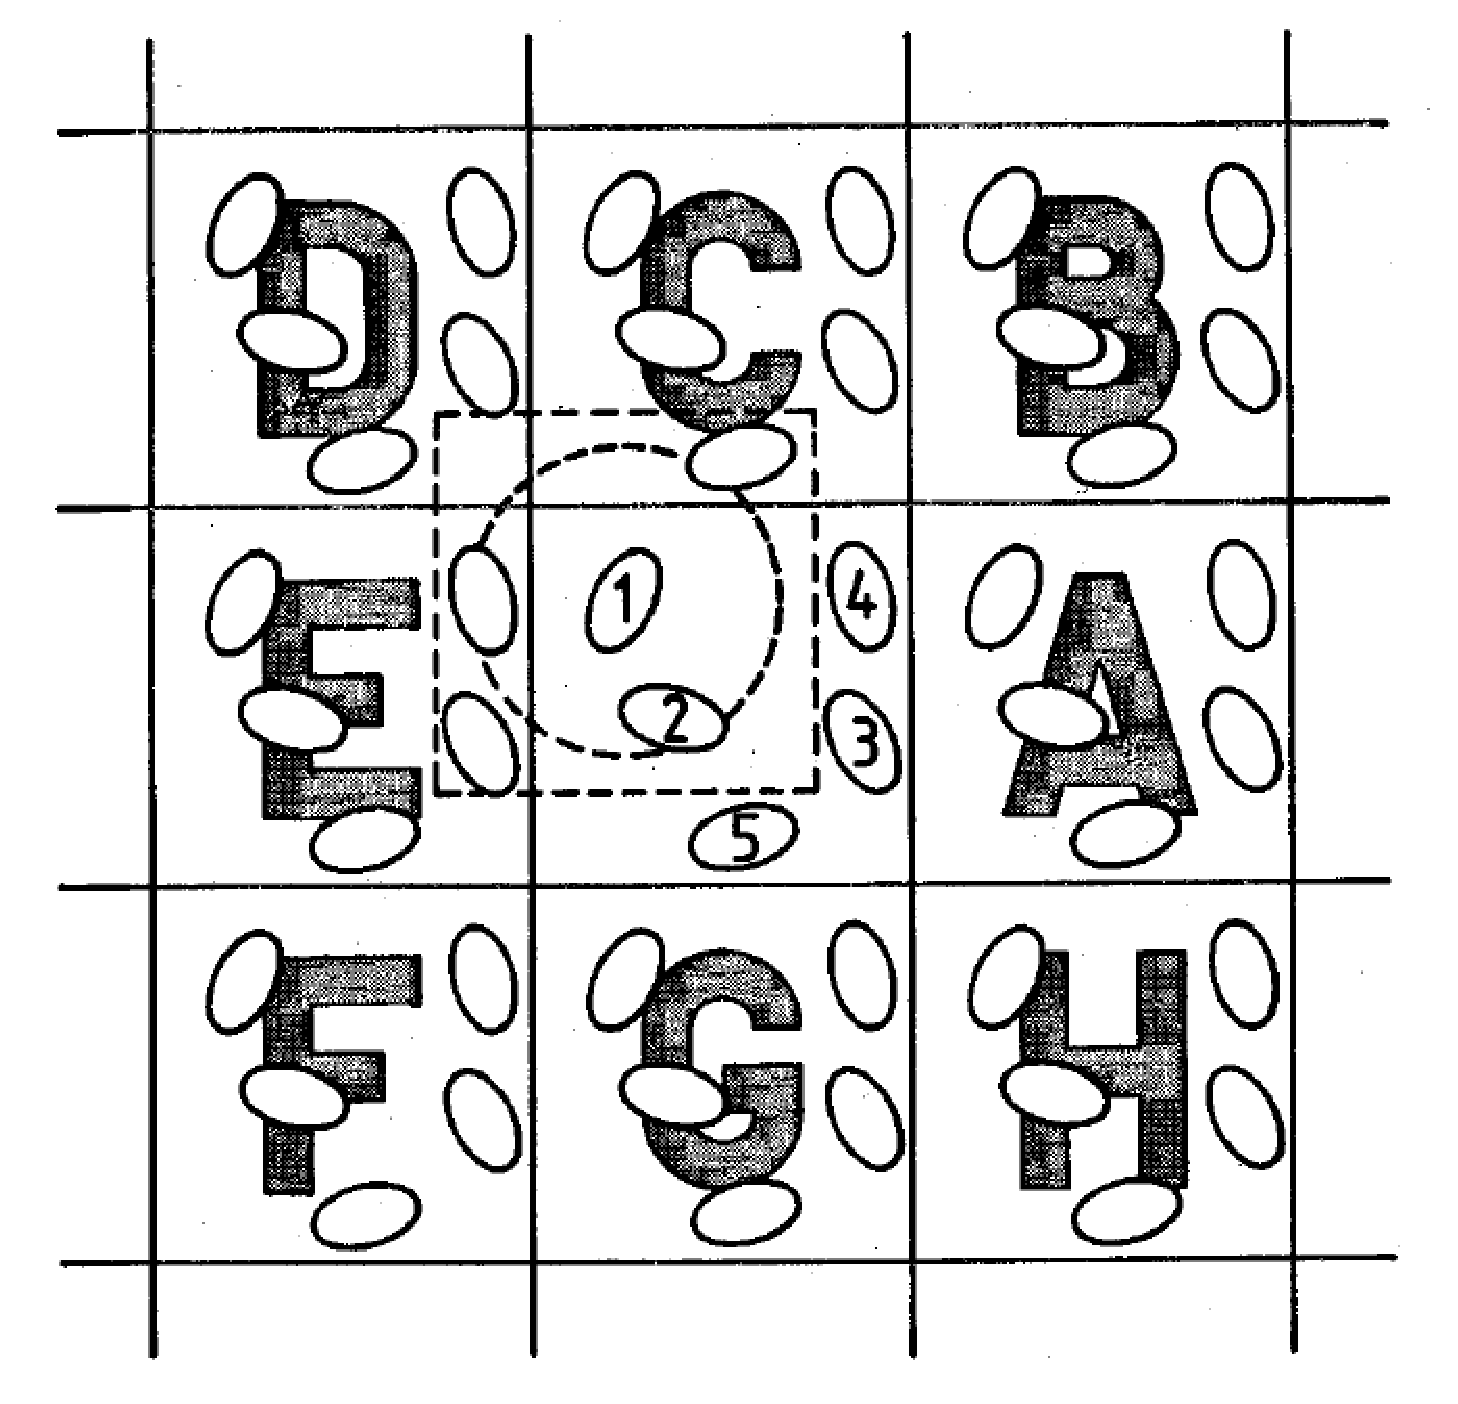
\includegraphics[scale=0.2]{pbc.eps}
\caption{{\scriptsize PBCs and minimum image convention [Allen \& Tildesley, Comp. Sim. of Liquids]}}
\end{figure}

\end{frame}

%%%%%%%%%%%%%%%%% NEW  SLDE

\begin{frame}\frametitle{Electrostatic interactions: Ewald method}

The elecrostatic energy for a periodic system can be written as\footnote{{\scriptsize Adv. Polym. Sci.,  {\bf
185 }, 59 (2005)}},

\begin{equation}
	E= \frac{1}{2} \sum_{m \in \mathbb{Z}^3}^{\infty} \sum_{i,j=1}^{N}{}^{'} \frac{q_i q_j}{ |\mathbf{r}_{ij} + \mathbf{m}L| }
\end{equation}

where $\mathbf{r}_{ij} = \mathbf{r}_i -   \mathbf{r}_j$, $\mathbf{m}$ refers to the periodic 
images. Primed summation means $i=j$ interaction is excluded for $\mathbf{m}=0$.

$q_x$ is the partial charge on atom $x$.

\only<2> { 
The potential is splitted such that,

\begin{equation}
	\frac{1}{r} = \frac{f(r)}{r} + \frac{1-f(r)}{r}
\end{equation}
}

\only<3> { 
givig rise to the total energy:

\begin{equation}
	E = E^{(r)} +  E^{(k)} +  E^{(s)} +  E^{(d)}
\end{equation}
}

\end{frame}

%%%%%%%%%%%%%%%%% NEW  SLDE
\begin{frame}\frametitle{Electrostatic interactions}

\begin{equation}
	E^{(r)}  = \frac{1}{2} \sum_{m \in \mathbb{Z}^3}^{\infty} 
	\sum_{i,j=1}^{N}{}^{'} q_i q_j\frac{\textrm{erfc}(\alpha |\mathbf{r}_{ij} 
	+ \mathbf{m}L| )}{ |\mathbf{r}_{ij} + \mathbf{m}L| }
\end{equation}
\begin{equation}
	E^{(k)}  = \frac{1}{2V} \sum_{k \ne 0} \frac{4 \pi}{k^2} e^{k^2/4 \alpha^2} 
	|\tilde{\rho} (\mathbf{k})|^2 
\end{equation}
\begin{equation}
	E^{(s)}  = - \frac{\alpha}{\sqrt{\pi}} \sum_{i} q_i^2 
\end{equation}
\begin{equation}
	E^{(d)}  =  \frac{2 \pi}{(1+2\epsilon')V} (\sum_{i} q_i \mathbf{r}_i )^2 
\end{equation}
\end{frame}

%%%%%%%%%%%%%%%%%% NEW  SLDE
%\begin{frame}\frametitle{Electrostatic interactions: Cutoff methods}
%
%The elecrostatic energy for a periodic system can be written as\footnote{{\scriptsize Adv. Polym. Sci.,  {\bf
%185 }, 59 (2005)}},
%
%\begin{equation}
%	E= \frac{1}{2} \sum_{m \in \mathbb{Z}^3}^{\infty} \sum_{i,j=1}^{N}{}^{'} \frac{q_i q_j}{ |\mathbf{r}_{ij} + \mathbf{m}L| }
%\end{equation}
%
%where $\mathbf{r}_{ij} = \mathbf{r}_i -   \mathbf{r}_j$, $\mathbf{m}$ refers to the periodic 
%images. Primed summation means $i=j$ interaction is excluded for $\mathbf{m}=0$.
%
%Can we truncate the interactions up to $\mathbf{r}=R_c$?
%
%\begin{equation}
%	E =  \frac{1}{2} \sum_i^N \sum_{j}^{\mathbf{r}_{ij}<R_c} \frac{1}{\mathbf{r}_{ij}}  + \Phi 
%\end{equation}
%
%\end{frame}

%%%%%%%%%%%%%%%%% NEW  SLDE

%\begin{frame}\frametitle{Electrostatic interactions: NaCl lattice}
%
%\fboxsep=0pt
%\noindent %\fbox{%
%\begin{minipage}[t]{0.48\linewidth}
%\begin{figure}
%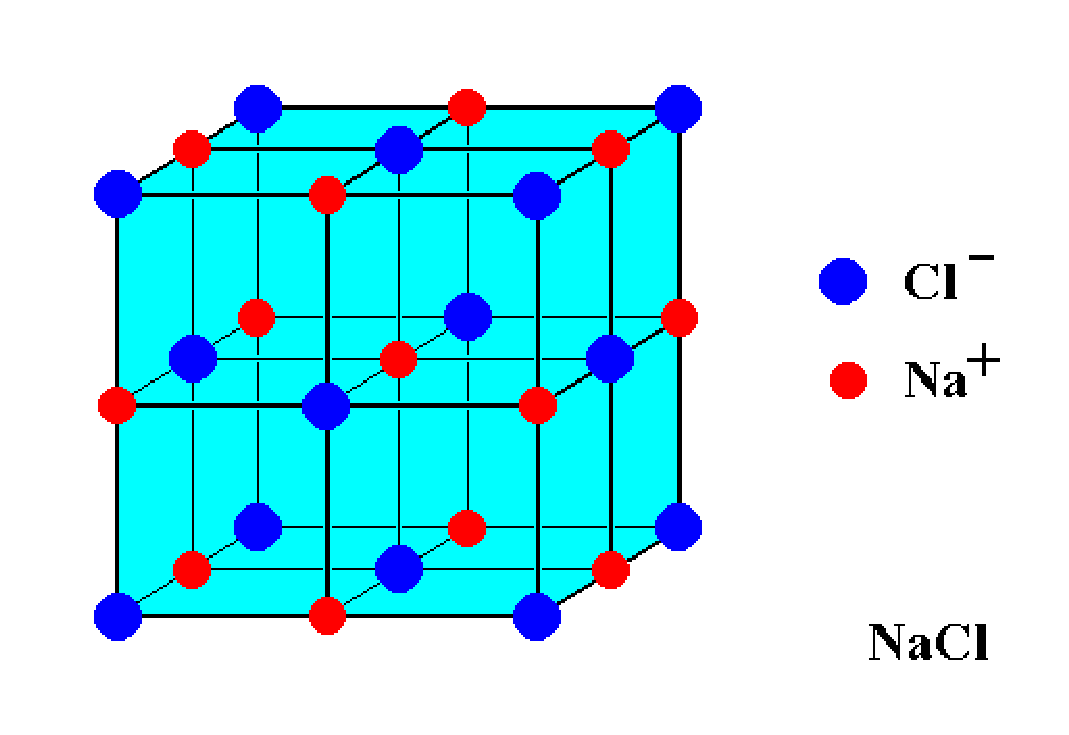
\includegraphics[scale=0.19]{nacl_complex_motif_2.eps}
%\caption{{\scriptsize  NaCl lattice. (source:goo.gl/Fa7tcL) }}
%\end{figure}
%\begin{equation}
%        E_i(R_c) = \sum_{\substack{j \neq i \\ (r_{ij}<R_c)}} \frac{q_i q_j}{r_{ij}} 
%\end{equation}
%
%%\begin{equation}
%$	E^{Mad} = -3.495129 ... q^2/a$
%%\end{equation}
%
%
%\end{minipage}
%\hfill%
%\begin{minipage}[t]{0.48\linewidth}
%\only<1>{
%\begin{figure}
%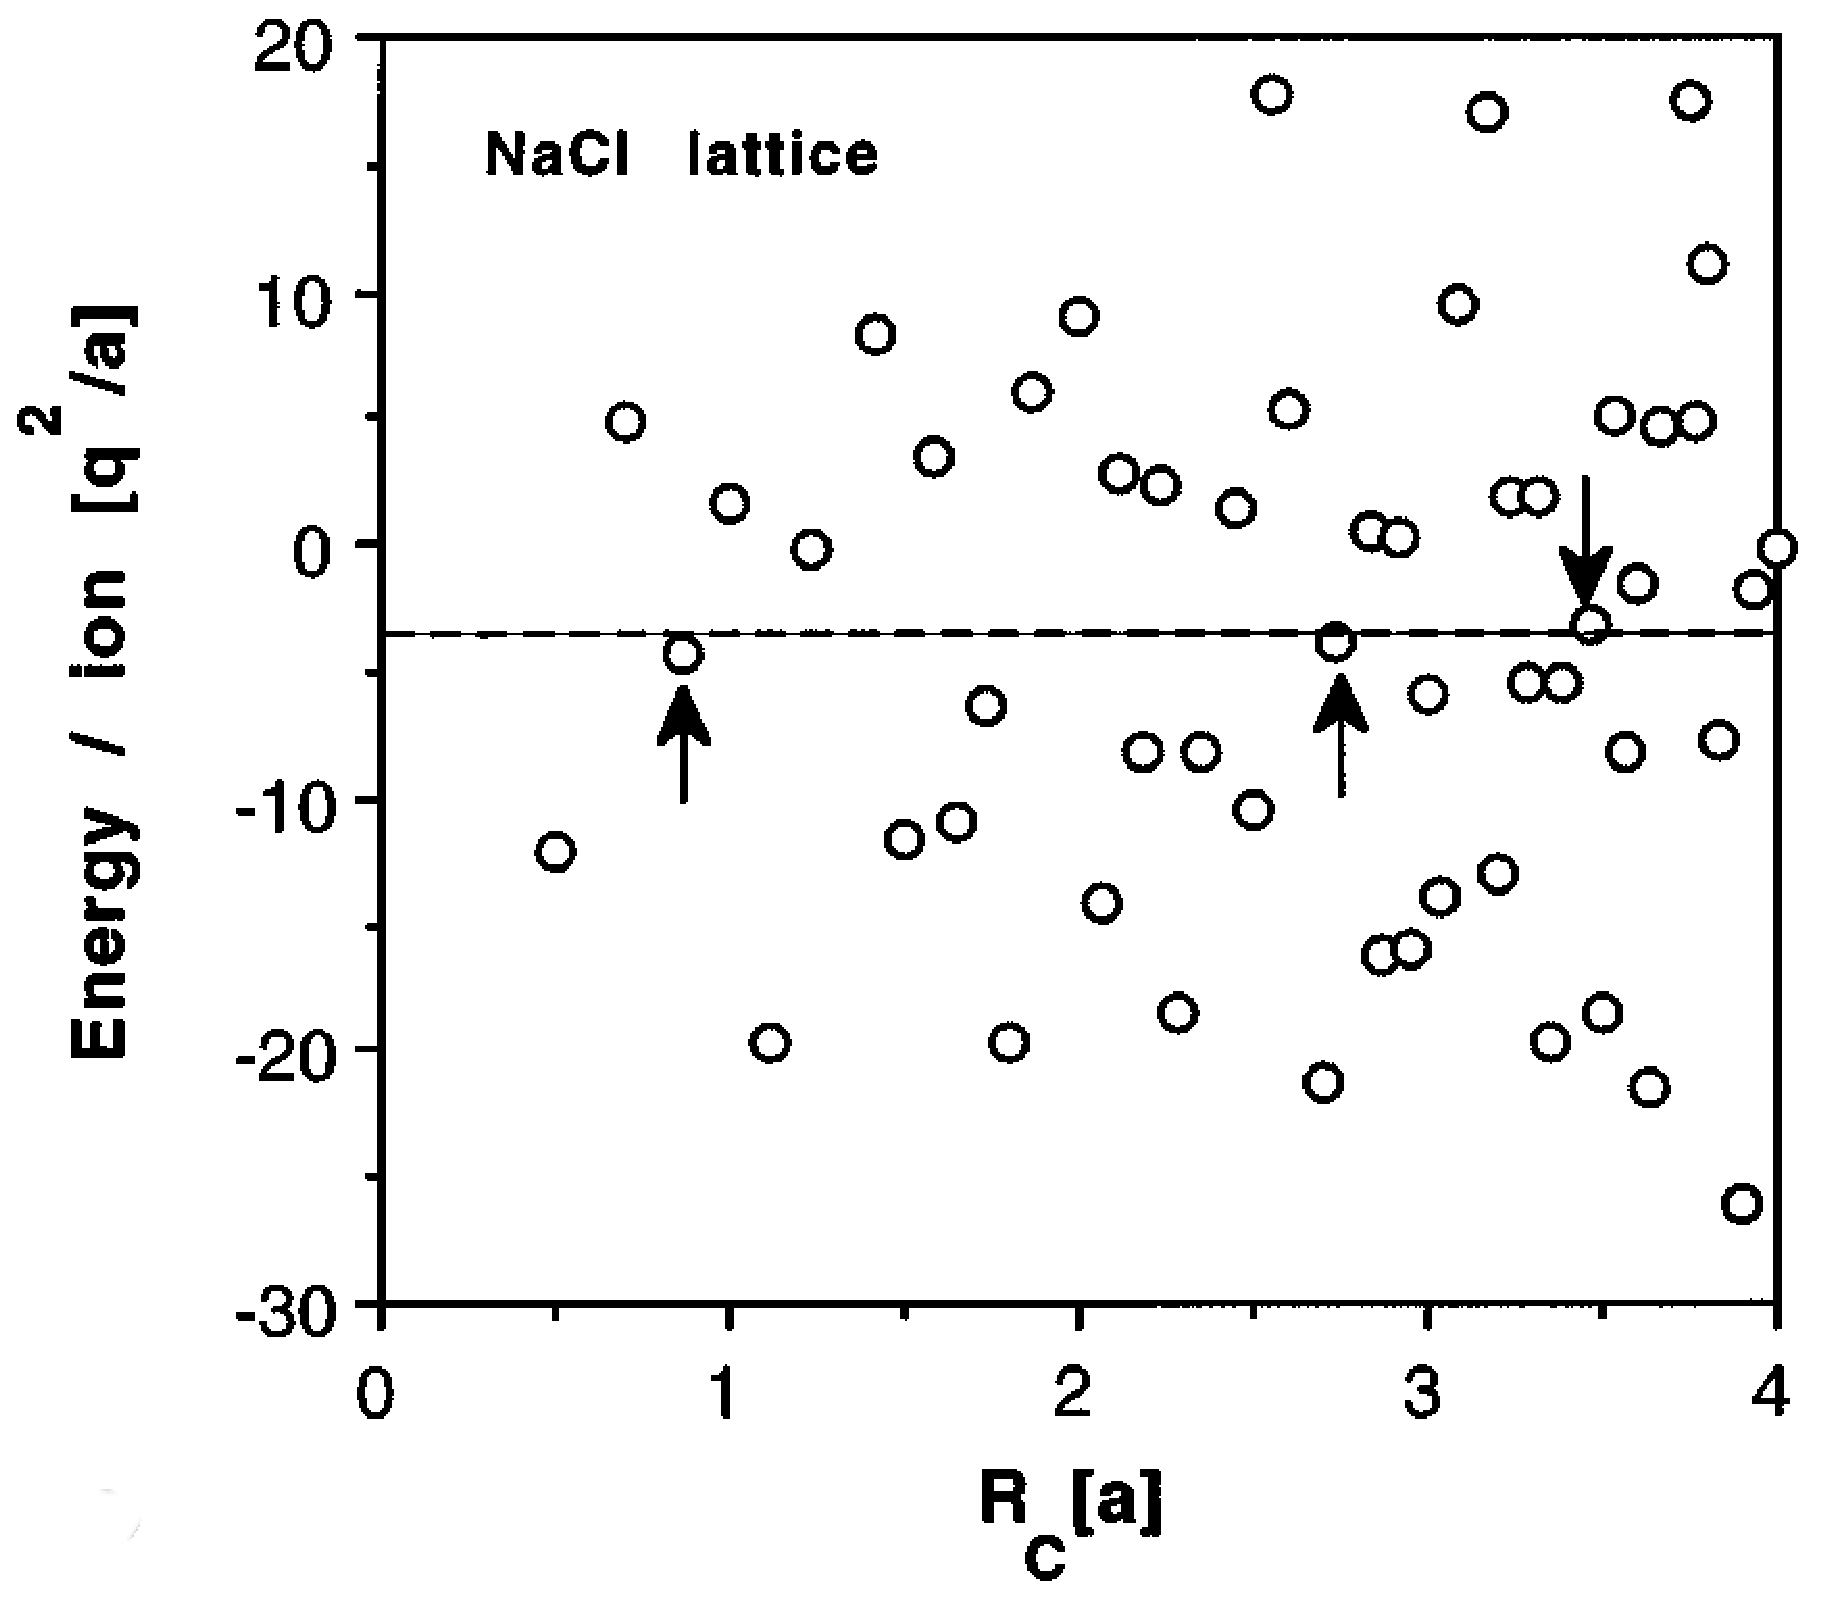
\includegraphics[scale=0.14]{rock-salt.eps}
%\caption{{\scriptsize  Single ion energy for NaCl lattice. (Wolf et al., JCP,
%{\bf 110}, 8256 (1999) ) }}
%\end{figure}
%}
%\only<2>{
%\begin{figure}
%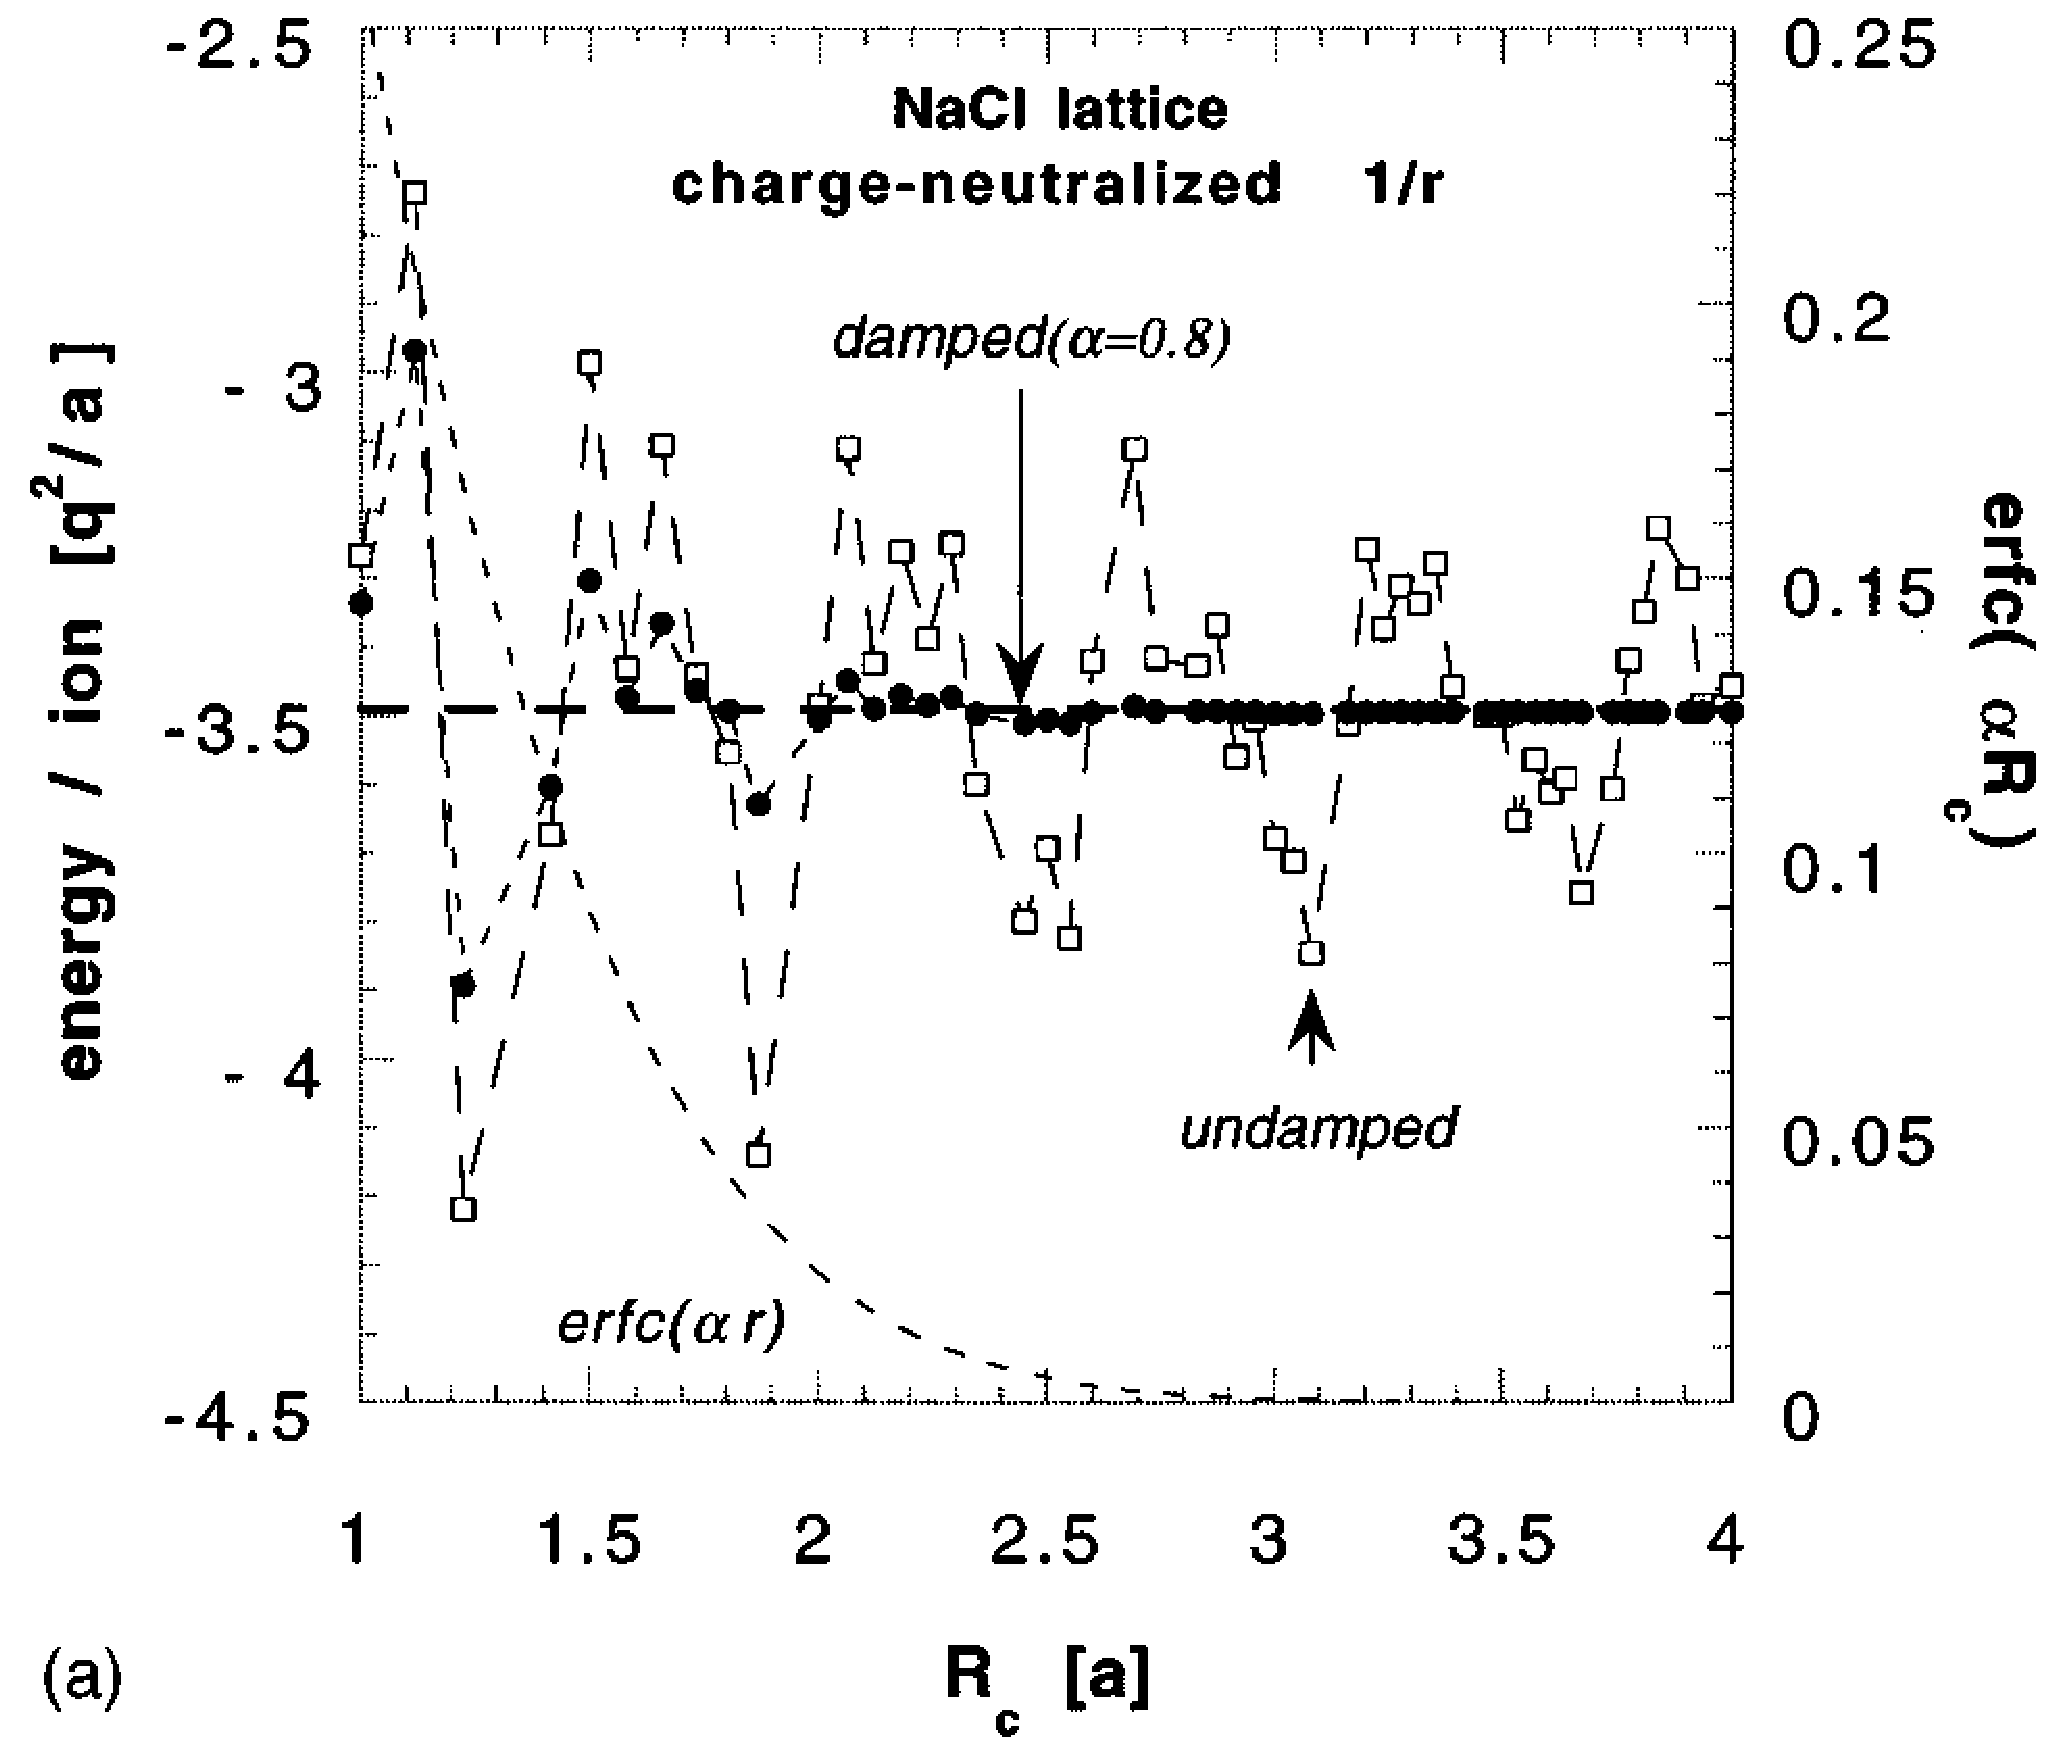
\includegraphics[scale=0.14]{wolf_convergence.eps}
%\caption{{\scriptsize  Energy convergence upon charge neutralization. (Wolf et al., JCP,
%{\bf 110}, 8256 (1999) ) }}
%\end{figure}
%}
%
%\end{minipage}
%
%\end{frame}

%%%%%%%%%%%%%%%%% NEW  SLDE
%\begin{frame}\frametitle{Isotropic Periodic Sum method: NaCl lattice}
%
%\fboxsep=0pt
%\noindent %\fbox{%
%\begin{minipage}[t]{0.48\linewidth}
% 
%\begin{equation}                                                                                                                                            
%\label{Eq:ipspot}
%\epsilon^{\text{IPS}}_{ij}(r_{ij})= \left\{ \begin{array}{l l} \epsilon _{ij}(r_{ij}) + \phi_{ij}(r_{ij}) & \quad \\
%\text{if $r_{ij}\le R_\text{c}$ } & \quad \\ 0 \text{~~otherwise} & \quad \end{array} \right.
%\end{equation}
%$\epsilon_{ij}$ is the Coulombic term and $\phi_{ij}$ is the long-range
%IPS correction  whose operational expression is given by, 
% 
%\begin{equation}
%\label{Eq:ipslong}
%\phi_{ij}(r_{ij}) = \frac{q_i q_j}{R_\text{c}} \left [ \sum^{6}_{k=1} b_{2k} \left ( \frac{r_{ij}}{R_\text{c}} \right )^{2k} \right ]
%\end{equation}
%\end{minipage}
%\hfill%
%\begin{minipage}[t]{0.48\linewidth}
%\begin{figure}
%\includegraphics[scale=0.21]{../hp_alp08_grid48000.eps}
%\caption{{\scriptsize Single ion energy using different cutoff methods. [ 
%JCP, {\bf 140}, 164106 (2014), JCP, {\bf 122}, 044107 (2005) ] }}
%\end{figure}
%\end{minipage}
%\end{frame}

%%%%%%%%%%%%%%%%% NEW  SLDE
\begin{frame}\frametitle{Integration of Newton's equation}

We now now the force field and we know the law of motion:
  \begin{equation}
	  \mathbf{F}= m \mathbf{a} = - \mathbf{\nabla} U      \mathrm{~~~~~~~~~~Newton's~ Law}
  \end{equation}

  we need to integrate this equation, here we use the leap-frog scheme [Hockney, 1970] ,

  \begin{equation}
	  \mathbf{r} (t+\delta t)= \mathbf{r} (t) + \delta t  \mathbf{v} (t+ \frac{1}{2} \delta t)
  \end{equation}

  \begin{equation}
	  \mathbf{v} (t+ \frac{1}{2}\delta t)= \mathbf{v} (t- \frac{1}{2} \delta t) + \delta t \mathbf{a}
  \end{equation}

velocities are updated according to, 

  \begin{equation}
	  \mathbf{v} (t)= \frac{1}{2} \left( \mathbf{v} (t+ \frac{1}{2} \delta t) + \mathbf{v} (t- \frac{1}{2} \delta t)  \right)
  \end{equation}

\end{frame}

%%%%%%%%%%%%%%%%% NEW  SLDE
\begin{frame}\frametitle{Constraints}

Collision of two diatomic molecules
\begin{minipage}[t]{0.48\linewidth}
\begin{figure}
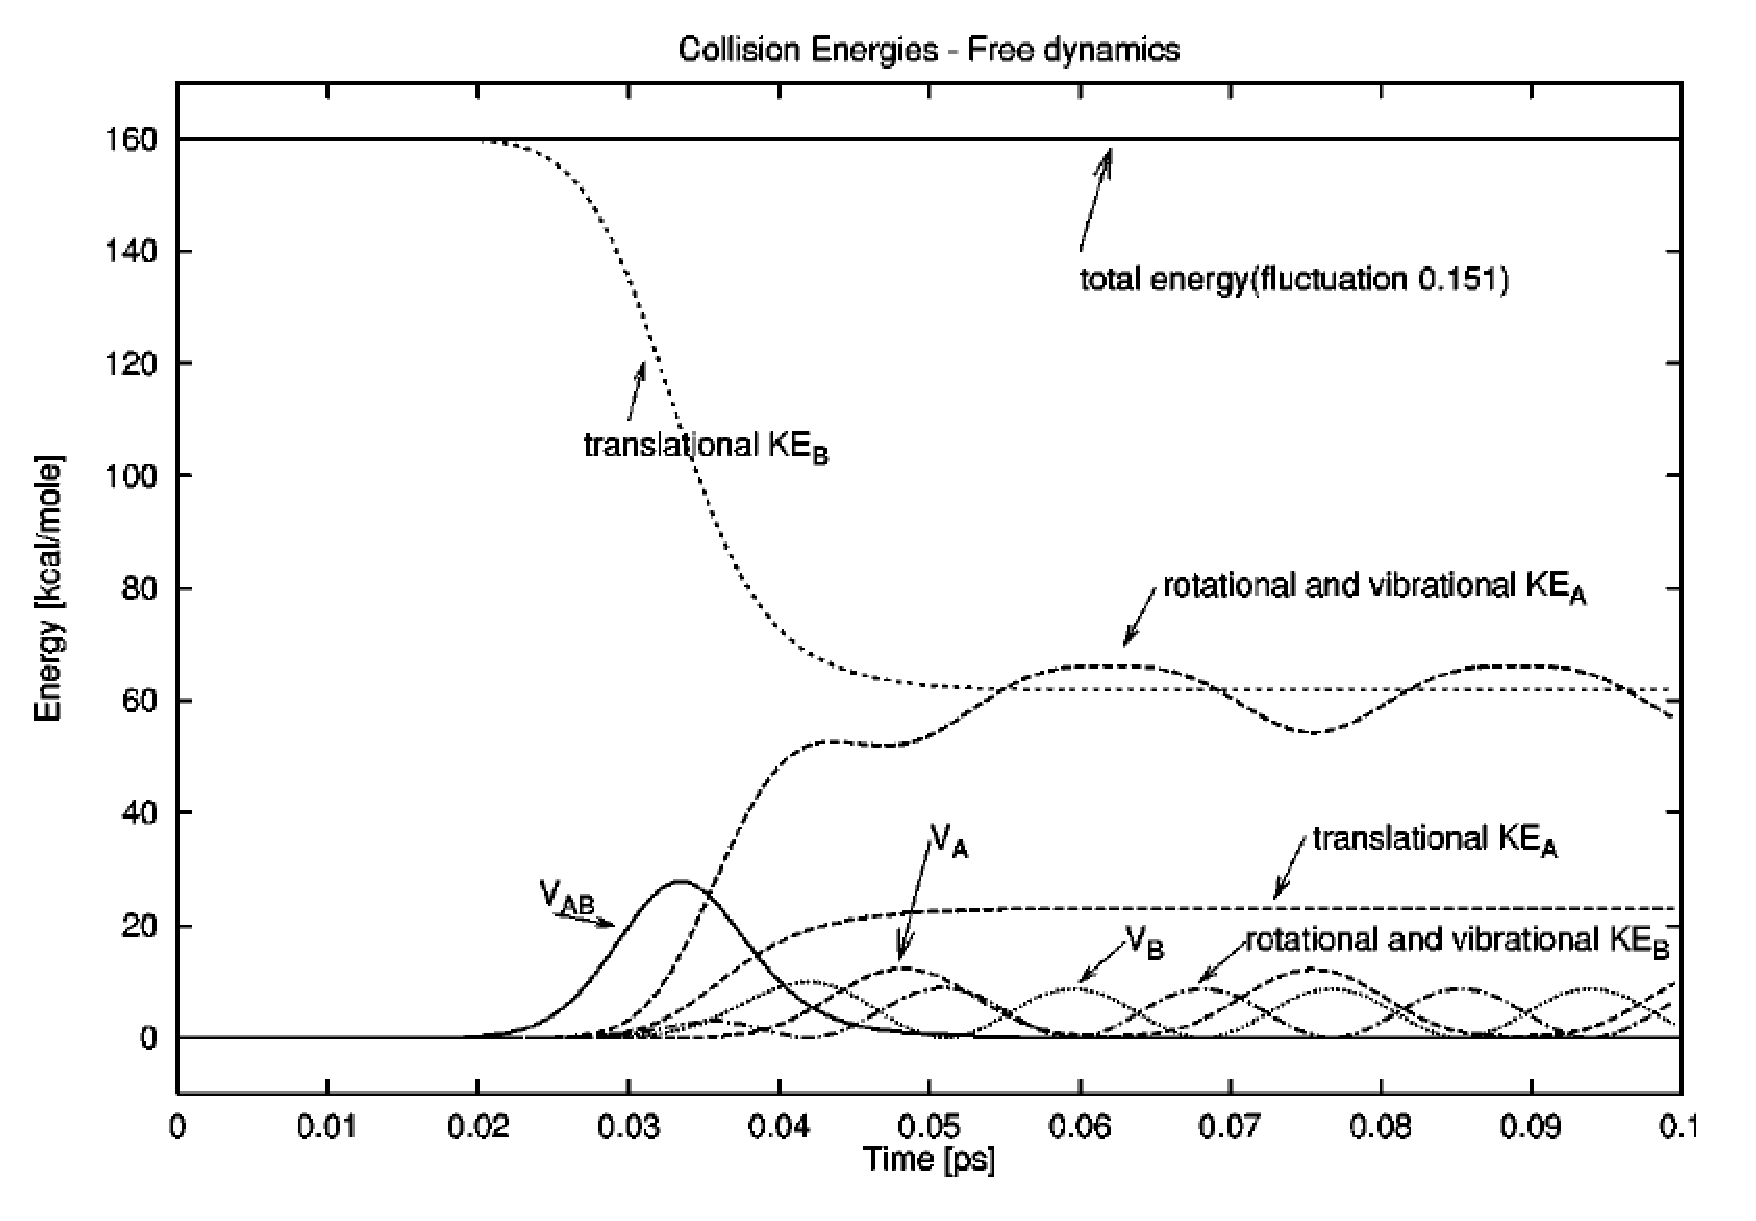
\includegraphics[scale=0.18]{collision.eps}
\caption{{\scriptsize  Free collision.}}
\end{figure}

\end{minipage}
%}%
\hfill%
%\fbox{%
\begin{minipage}[t]{0.48\linewidth}
\begin{figure}
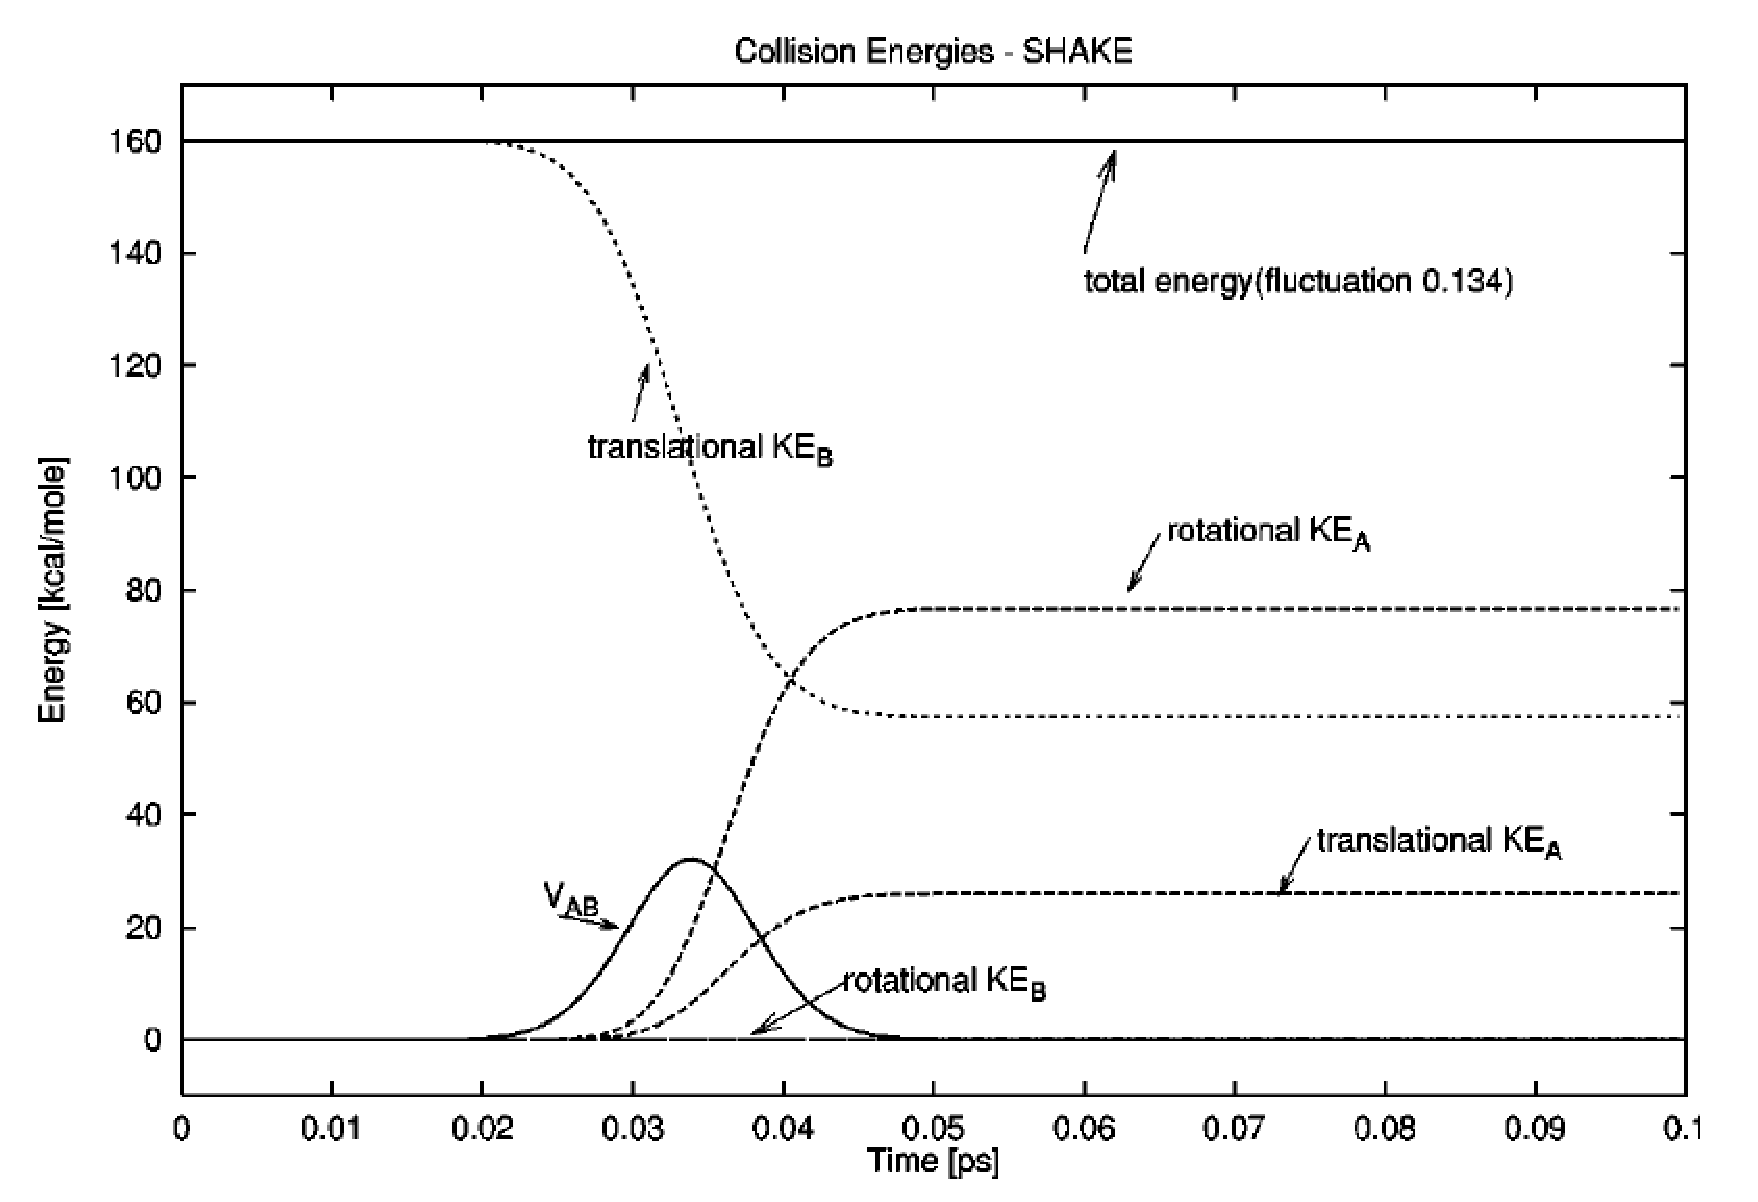
\includegraphics[scale=0.18]{collision_shake.eps}
\caption{{\scriptsize  SHAKE constraint.}}

\end{figure}
\end{minipage}
See JCP, {\bf 112}, 7919 (2000)
\end{frame}

%%%%%%%%%%%%%%%%% NEW  SLDE
\begin{frame}\frametitle{Constraints}

Modern approaches to deal with constraints
\begin{figure}
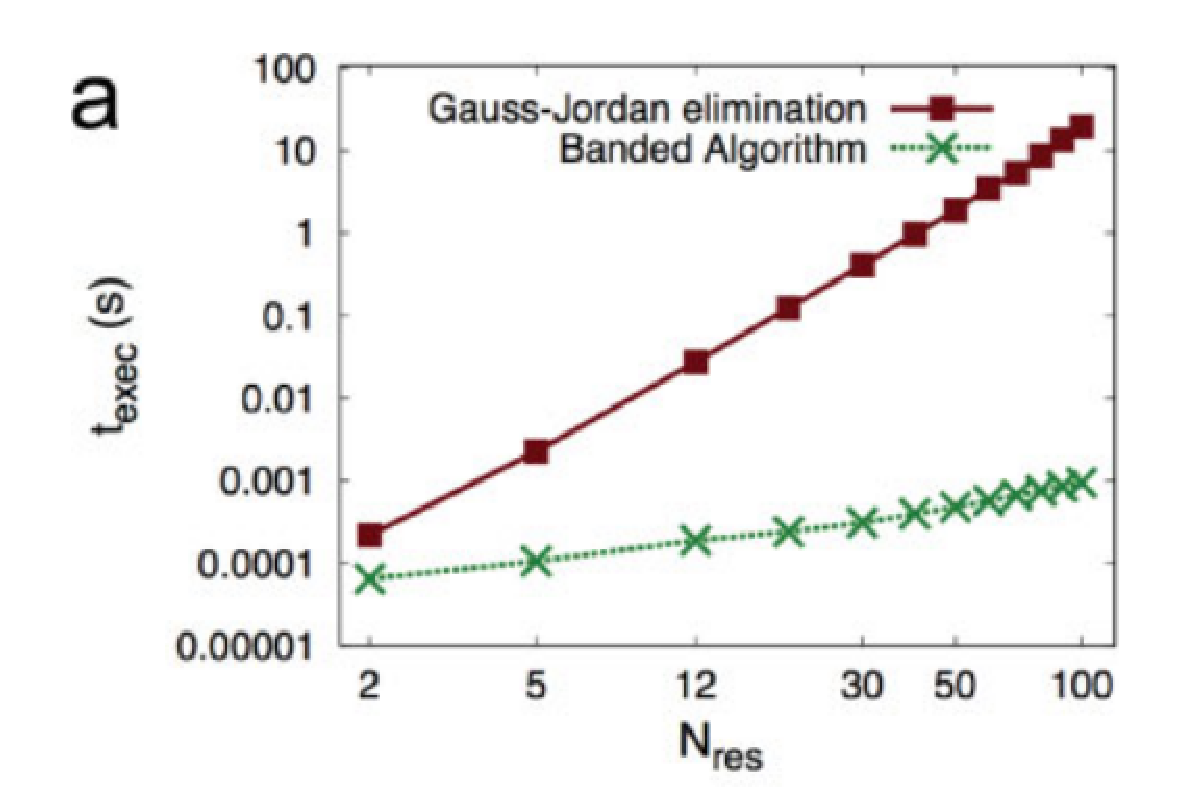
\includegraphics[scale=0.28]{ilves.eps}
\caption{{\scriptsize  ILVES method.}}
\end{figure}

See JCC, {\bf 32}, 3039 (2011)
\end{frame}

%%%%%%%%%%%%%%%%% NEW  SLDE
\begin{frame}[fragile]\frametitle{Techniques to speedup simulations}


\begin{minipage}[t]{0.48\linewidth}
	\begin{itemize}
        \item MPI parallelization	
	\item MPI+OpenMP parallelization
	\item Domain decomposition scheme
	\item Multiple communicators
	\end{itemize}

\begin{verbatim} 

do i=1,num_particles 
x(i) = x(i) + f(i)*dt 
enddo 

\end{verbatim}

\end{minipage}
%}%
\hfill%
%\fbox{%
\begin{minipage}[t]{0.48\linewidth}

\begin{figure} 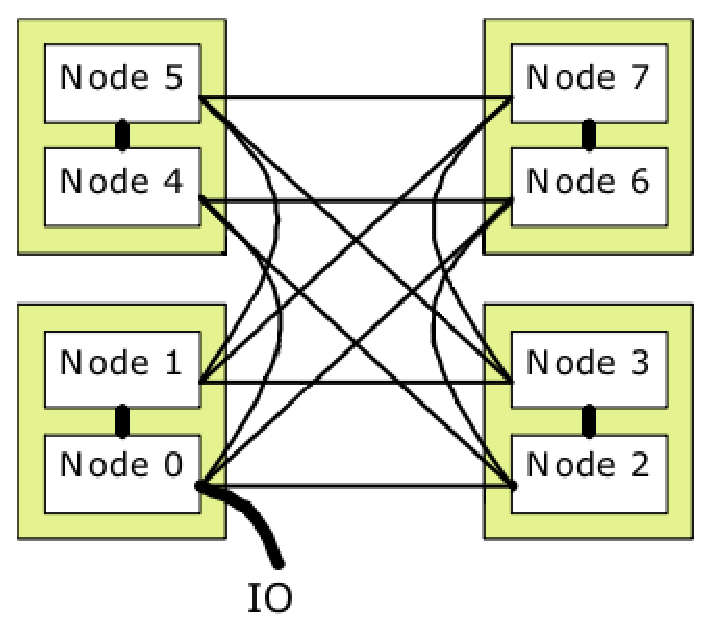
\includegraphics[scale=0.3]{../node_abisko.eps}
\caption{{\scriptsize  Nodes (MPI).}} \end{figure}

\begin{figure}
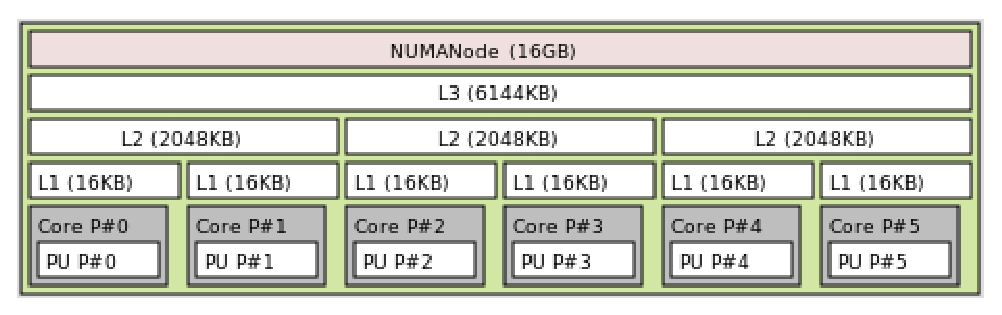
\includegraphics[scale=0.25]{../lstopoabisko128G1CU_0.eps} \caption{{\scriptsize
NUMA machine (OpenMP).}} \end{figure}

\end{minipage}
\end{frame}





%%%%%%%%%%%%%%%%% NEW  SLDE
\subsection{Ensembles} 

\begin{frame}\frametitle{Ergodicity}


\fboxsep=0pt
\noindent %\fbox{%
\begin{minipage}[t]{0.48\linewidth}

\begin{equation}
\begin{aligned}
\mathcal{A}_{obs} =  &  <\mathcal{A}>_{\mathrm{time}} \\
&= <\mathcal{A}(\Gamma (t))>_{\mathrm{time}}  \\
&= \lim_{t_{\mathrm{obs}} \rightarrow \infty } \int_0^{t_{\mathrm{obs}}}
\mathcal{A}(\Gamma (t)) dt
\end{aligned}
\end{equation}


\end{minipage}
\hfill%
\begin{minipage}[t]{0.48\linewidth}
\begin{figure}
\includegraphics[scale=0.06,angle=3.0]{coffee.eps}
\caption{{\scriptsize  Coffee cup. }}
\end{figure}

\end{minipage}

\end{frame}

%%%%%%%%%%%%%%%%% NEW  SLDE
\begin{frame}\frametitle{Statistical ensembles}

\begin{itemize}
\item Microcanonical ensemble (NVE) partition function is [Allen \& Tildesley, Comp. Sim. of Liquids],
	\begin{equation}
		Q_{NVE}= \frac{1}{N!}\frac{1}{h^{3N}} \int \textrm{d}\mathbf{r} \textrm{d}\mathbf{p} 
		\delta (\mathcal{H}(\mathbf{r},\mathbf{p}) -E)
	\end{equation}
	The thermodynamic potential is the negative of the entropy $-S/k_{B} = -\ln Q_{NVE}$

\item In the case of the Canonical ensemble (NVT) the partition function is,
	\begin{equation}
		Q_{NVT}= \frac{1}{N!}\frac{1}{h^{3N}} \int \textrm{d}\mathbf{r} \textrm{d}\mathbf{p} 
	        \exp (-\mathcal{H}(\mathbf{r},\mathbf{p})/k_B T)
	\end{equation}
	with thermodynamic potential $A/k_B T = -\ln Q_{NVT}$.


\end{itemize}

\end{frame}

%%%%%%%%%%%%%%%%% NEW  SLDE


\begin{frame}\frametitle{Statistical ensembles}

\begin{itemize}
\item Isothermal-isobaric ensemble (NPT) partition function is,
	\begin{equation}
		Q_{NPT}= \frac{1}{N!}\frac{1}{h^{3N}} \frac{1}{V_0} \int \textrm{d}V
		\int \textrm{d}\mathbf{r} \textrm{d}\mathbf{p} 
		\exp ( -(\mathcal{H}(\mathbf{r},\mathbf{p}) + PV)/k_BT)
	\end{equation}
	the corresponding thermodynamic potential is $G/k_{B} = -\ln Q_{NPT}$

\item Grand-canonical ensemble ($\mu$VT) partition function is,
	\begin{equation}
		Q_{\mu VT}= \sum_N \frac{1}{N!}\frac{1}{h^{3N}} \exp(\mu N/k_BT) 
		\int \textrm{d}\mathbf{r} \textrm{d}\mathbf{p} 
		\exp ( -\mathcal{H}(\mathbf{r},\mathbf{p}) /k_BT)
	\end{equation}
	the corresponding thermodynamic potential is $-PV/k_{B} = -\ln Q_{\mu VT}$

\end{itemize}

\end{frame}

%%%%%%%%%%%%%%%%% NEW  SLDE
\begin{frame}\frametitle{Thermostats}

\begin{itemize}
	\item NVE is obtained by solving NE.
	\item NVT can be achieved with the following thermostats: Berendsen, Velocity-rescaling,
		Nose-Hoover.

\begin{equation}
	H= \sum_{i=1}^{N} \frac{\mathbf{p}_i}{2m_i} + U(\mathbf{r}_1,\mathbf{r}_2,\ldots, \mathbf{r}_N) + \frac{p_{\xi}^2}{2Q} 
	+ N_f kT\xi
\end{equation}
 A better approach is Nose-Hoover chain.

	\item  Using general and local thermostats. 

	\item NPT can be simulated with Berendsen and Parrinello-Rahman methods.
\end{itemize}

\end{frame}


%%%%%%%%%%%%%%%%% NEW  SLDE
\subsection{Beyond classical MD} 
\subsubsection{Accelerated MD} 
\begin{frame}
\frametitle{Accelerated MD simulations}

The original potential energy surface $V(\mathbf{r})$ is modified according to,

\begin{equation}                                                                                                                                            
\label{Eq:ipspot}          
V^*(\mathbf{r})= \left\{ 
\begin{array}{l l} V(\mathbf{r}), &  V(\mathbf{r}) \ge E, \quad \\
V(\mathbf{r}) + \Delta V(\mathbf{r})& V(\mathbf{r}) < E. \quad 
\end{array} \right.
\end{equation}

\begin{figure}
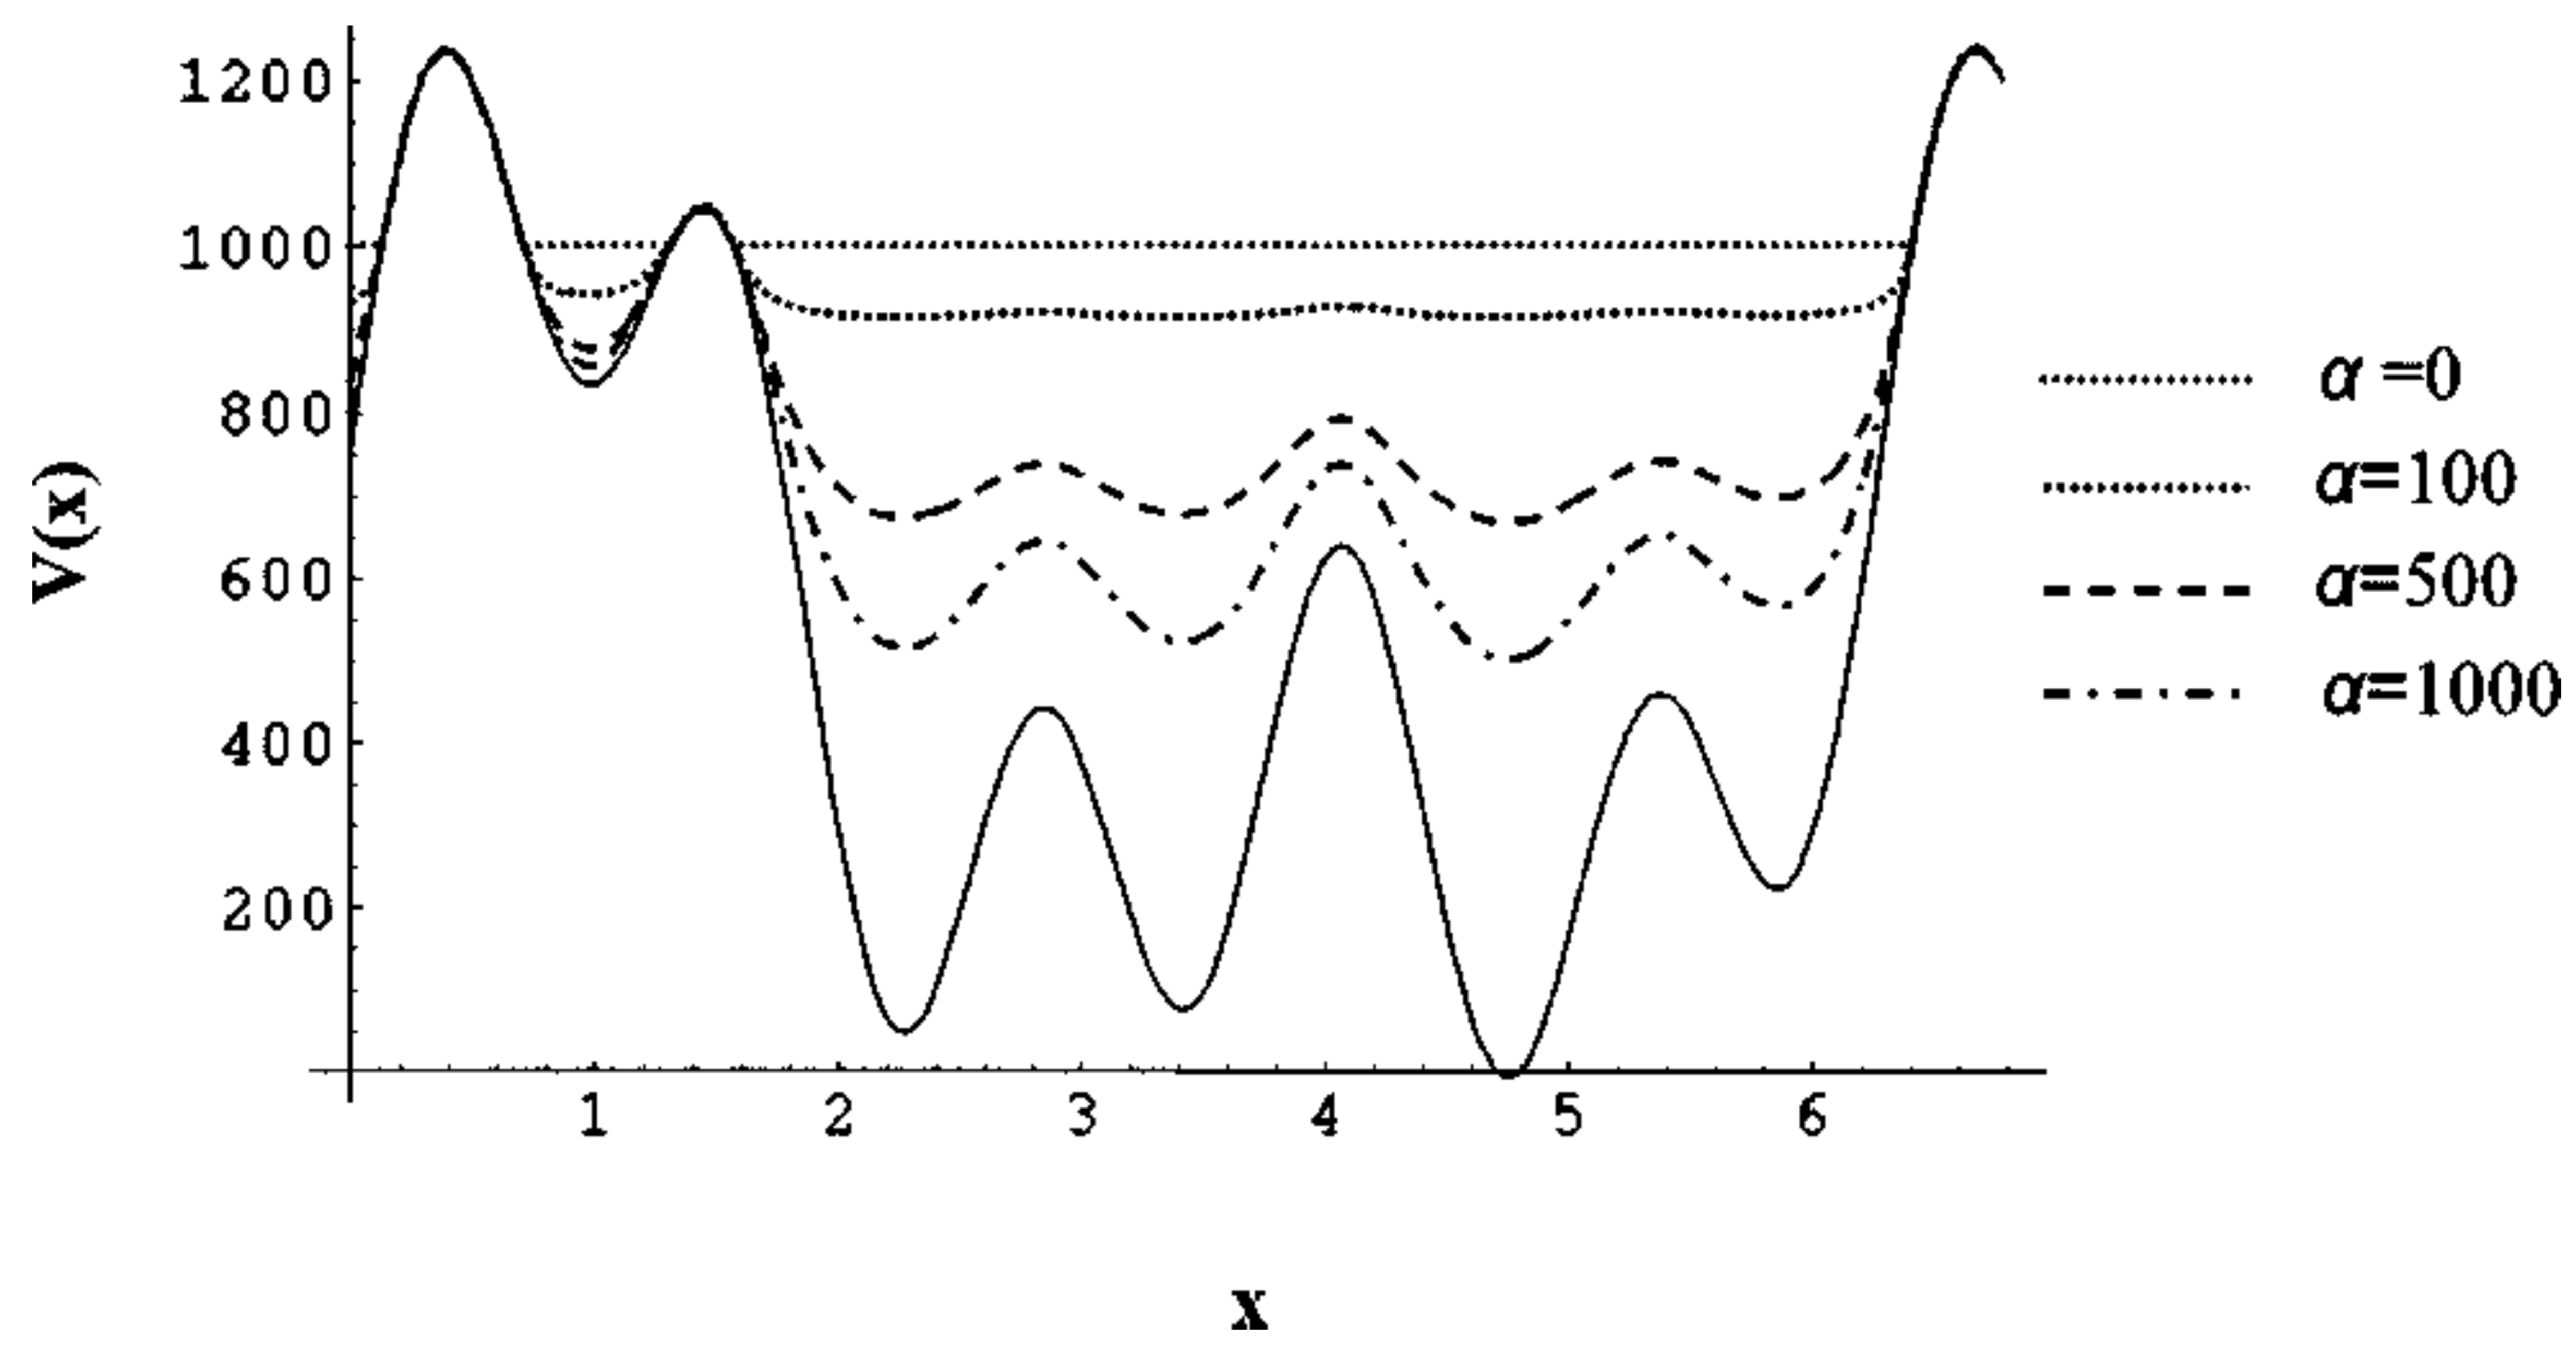
\includegraphics[scale=0.08]{accmd.eps}
\caption{{\scriptsize  Modified potential energy surface [JCP, {\bf 120}, 11919 (2004)]. }}
\end{figure}

\end{frame}

\begin{frame}
\frametitle{Accelerated MD simulations}

the biasing term is,

\begin{equation}                                                                                                                                            
\Delta V(\mathbf{r}) = \frac{ ( E-V(\mathbf{r}) )^2 }{ \alpha + ( E-V(\mathbf{r}) )}
\end{equation}

\begin{figure}
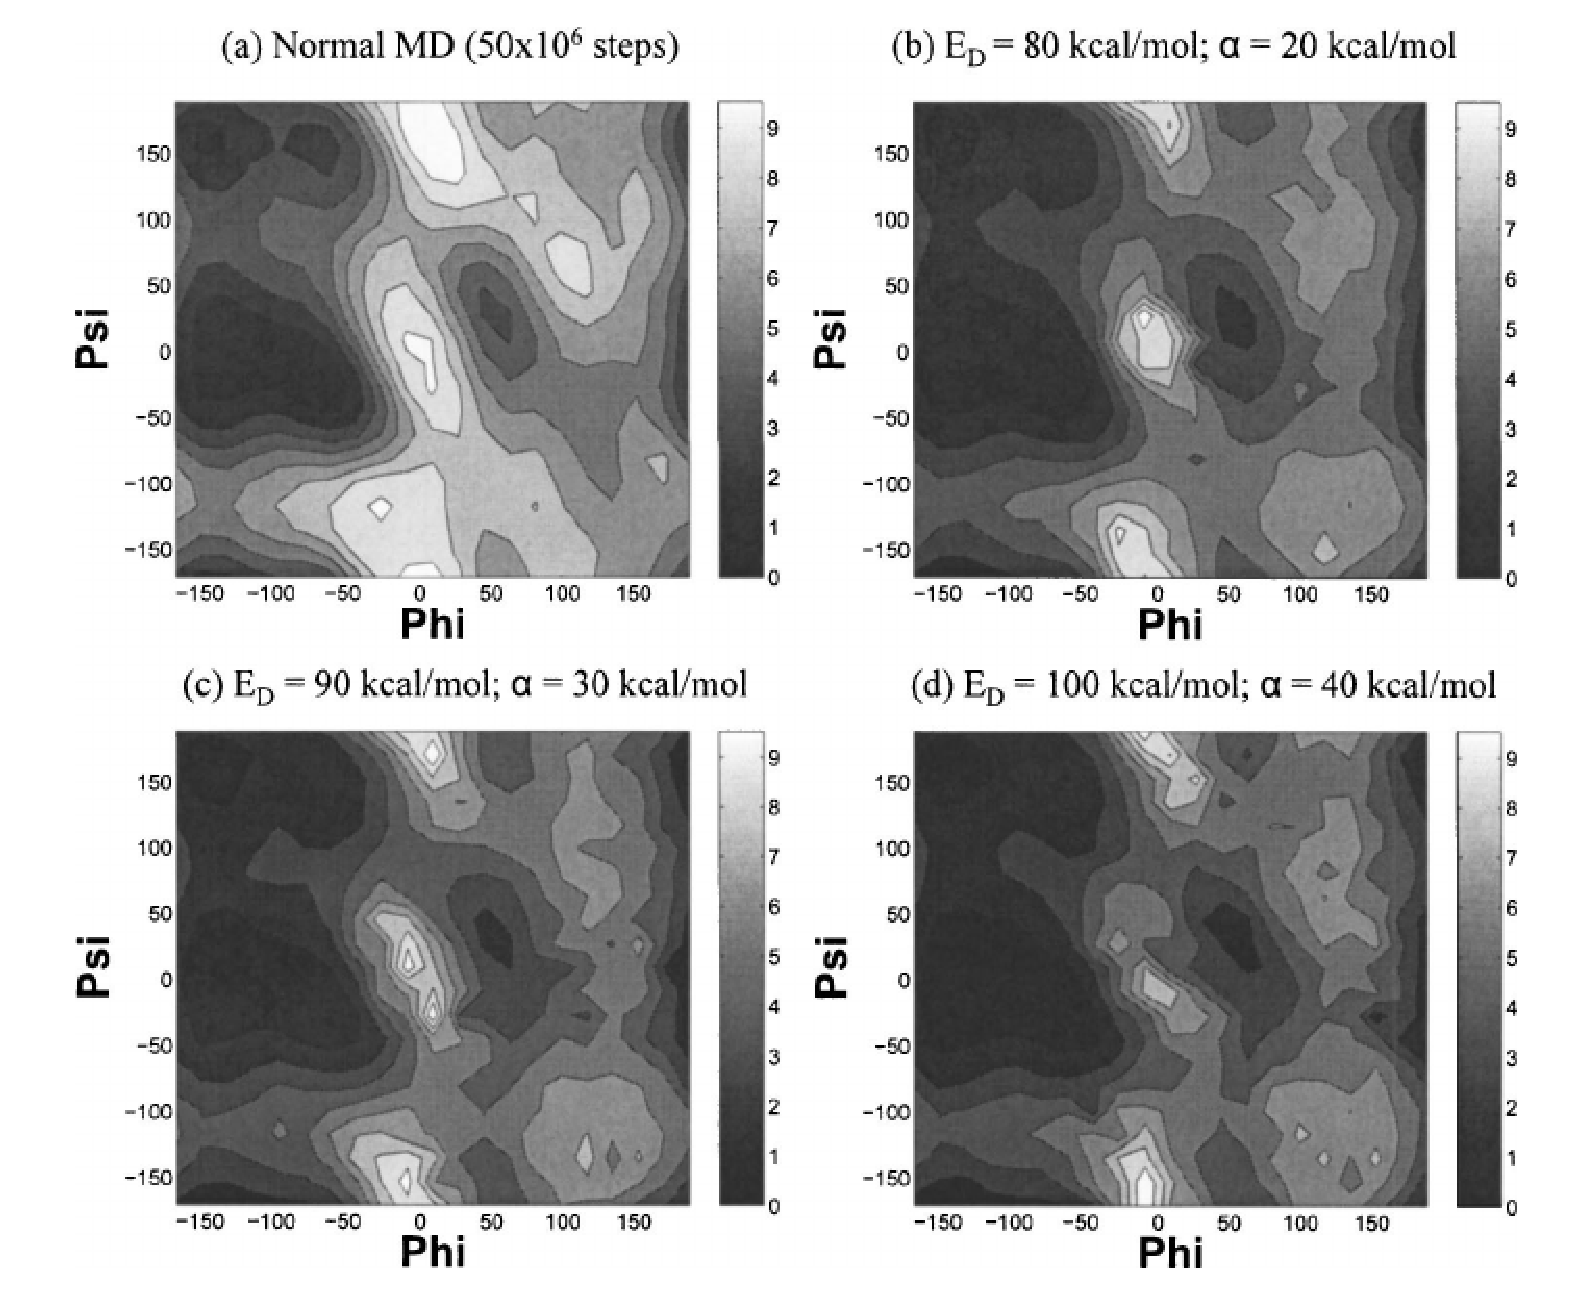
\includegraphics[scale=0.18]{accmd_fe.eps}
\caption{{\scriptsize Free energy landscape of Alanine dipeptide [JCP, {\bf 120}, 11919 (2004)]. }}
\end{figure}

\end{frame}



\subsubsection{Umbrella sampling} 

\begin{frame}
\frametitle{Umbrella sampling (US) simulations}
\only<1> { 
\FourQuad% 
{ The potential energy is modified as
follows~{\scriptsize JCP, {\bf 23}, 187 (1977)}:
\begin{equation*} E^{b}(r) = E^{u}(r)+w_i (\xi)
\end{equation*}

with  $w_i(\xi)=K/2(\xi -\xi^{ref}_i)^2$ 

}%
{\begin{figure}
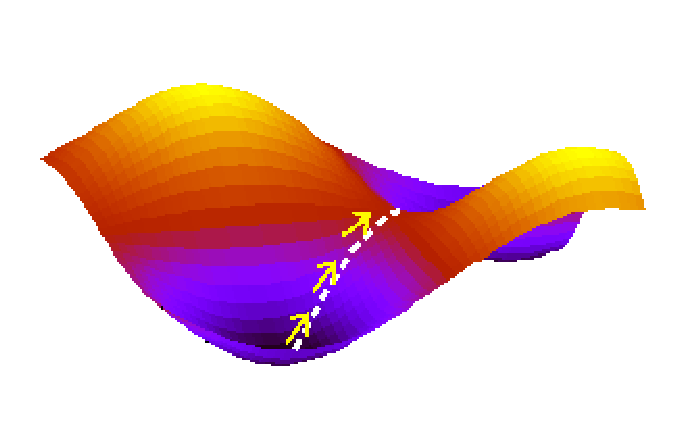
\includegraphics[scale=0.28]{surface_umbrella.eps}
\caption{{\scriptsize  Potential energy surface. }}
\end{figure}
}%
{

For each window the free energy is given by,
\begin{equation*}
A_i(\xi) = -(1/\beta) \ln P^b _i(\xi) - w_i(\xi) + F_i
\end{equation*}


}%
{
\begin{figure}
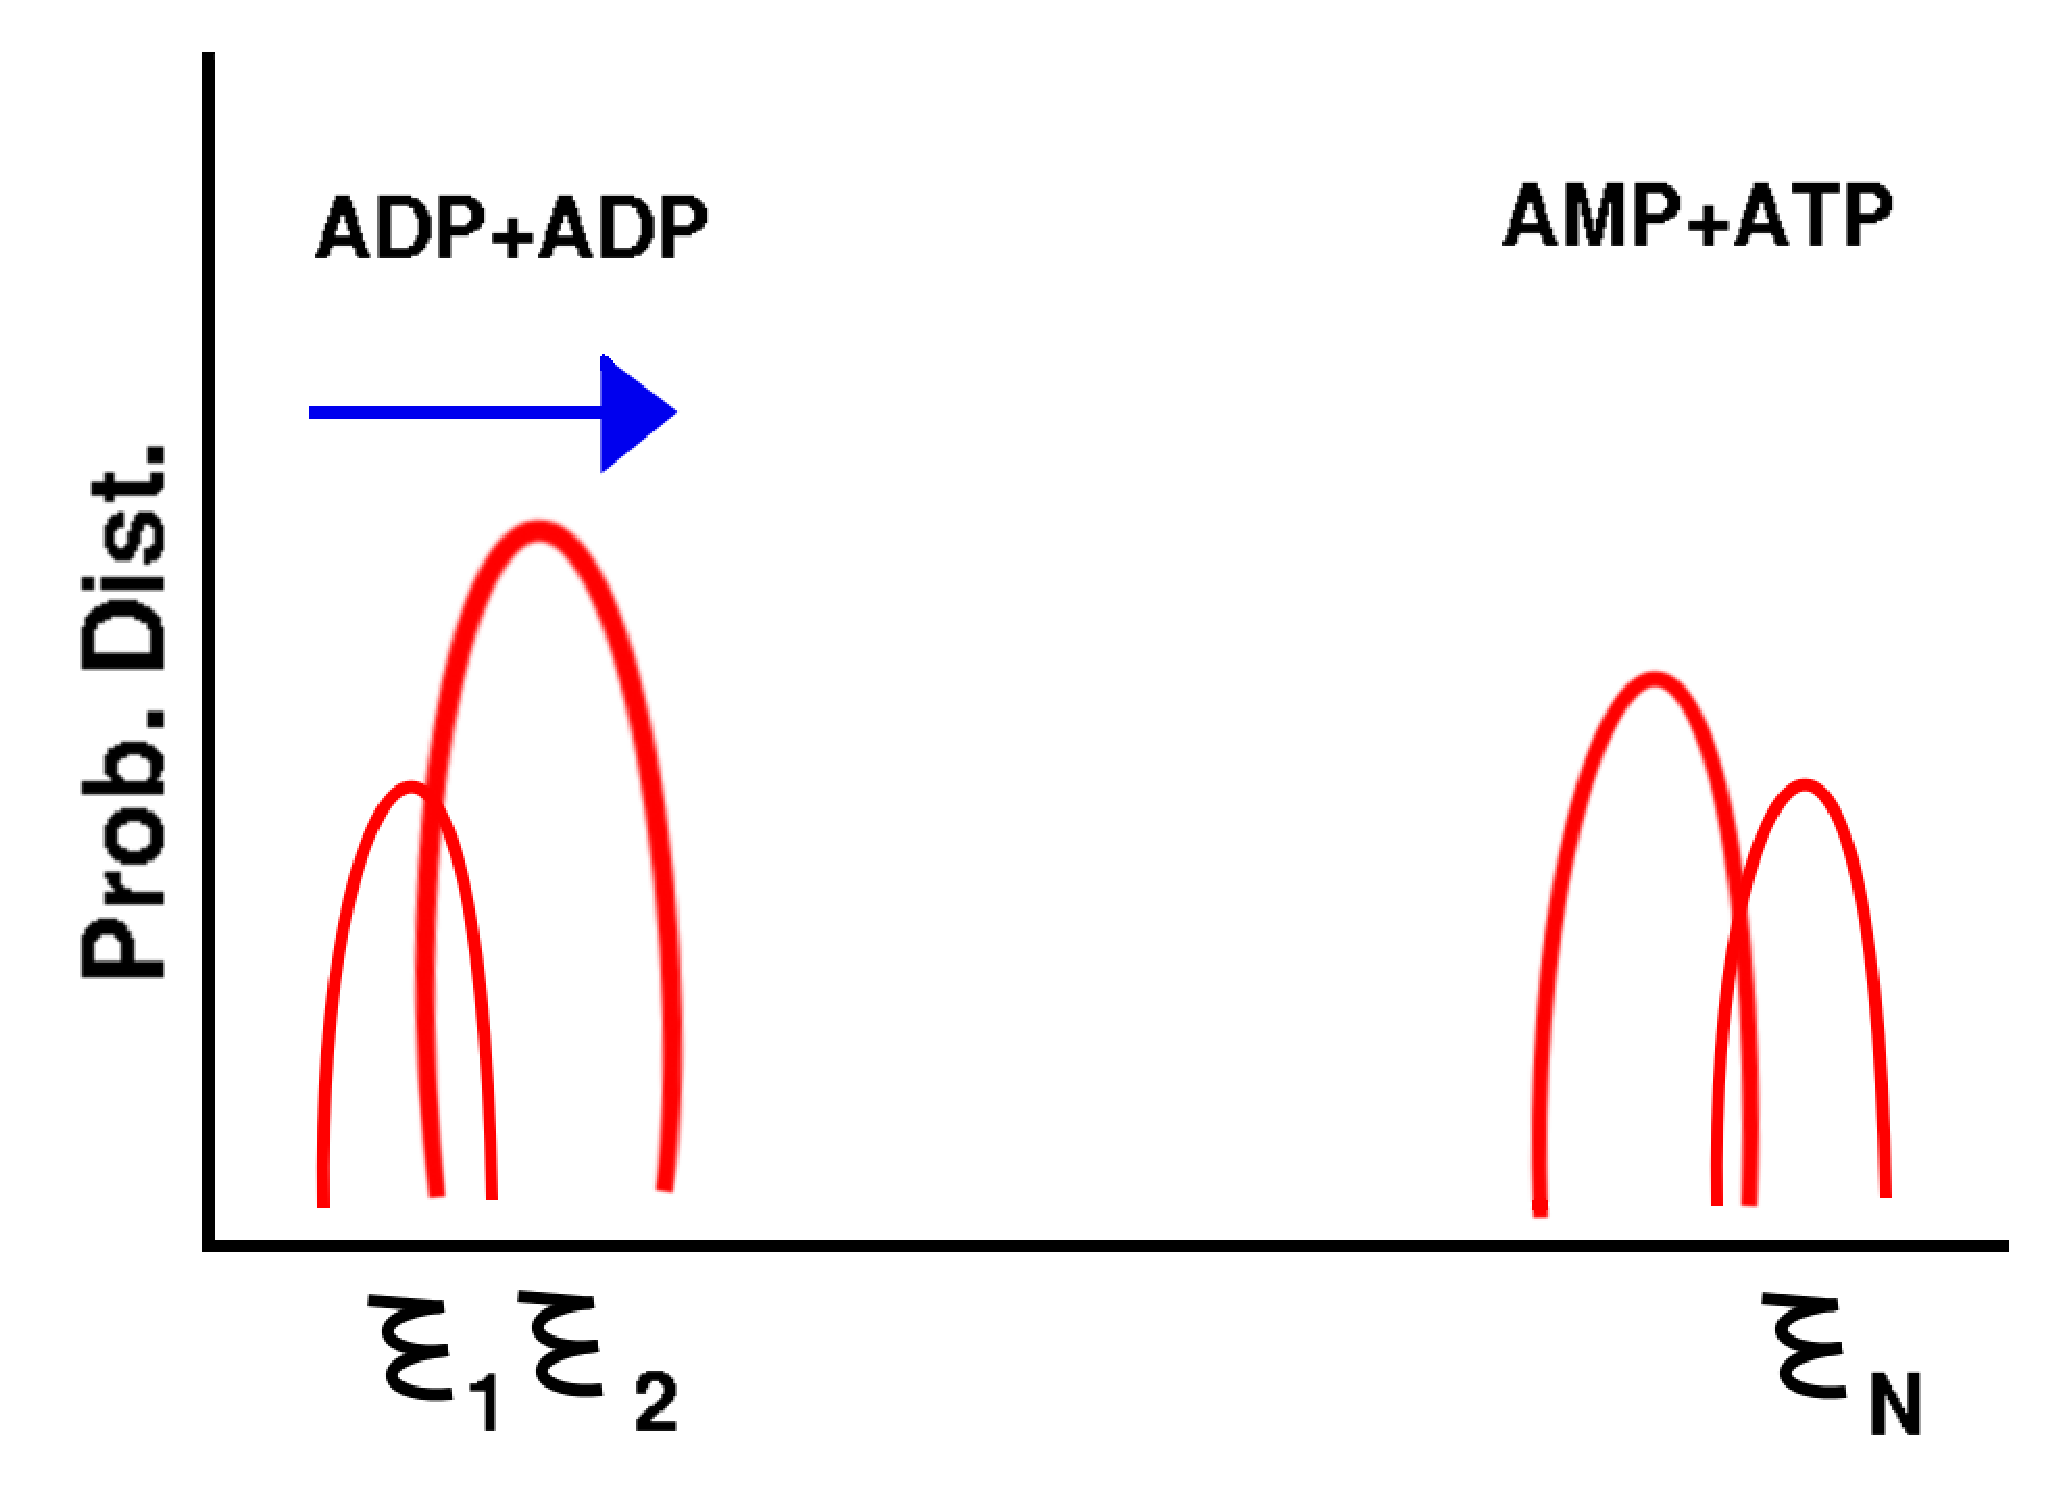
\includegraphics[scale=0.09]{prob_dist.eps}
\caption{{\scriptsize  Probability histograms. }}
\end{figure}
}
}
\end{frame}




\subsubsection{String method} 
\begin{frame}
\frametitle{String method (SM) simulations}
\FourQuad%
{
%First quadrant
Define a set of collective variables $z_j$ and  
effective forces as follows
\begin{equation*}
        \frac{k}{T} \int ^T_0 (z_j-\theta_j(t)) dt \sim \frac{\partial F(z)}{\partial z_j}
\end{equation*}
}%
{
%Second quadrant
\begin{figure}
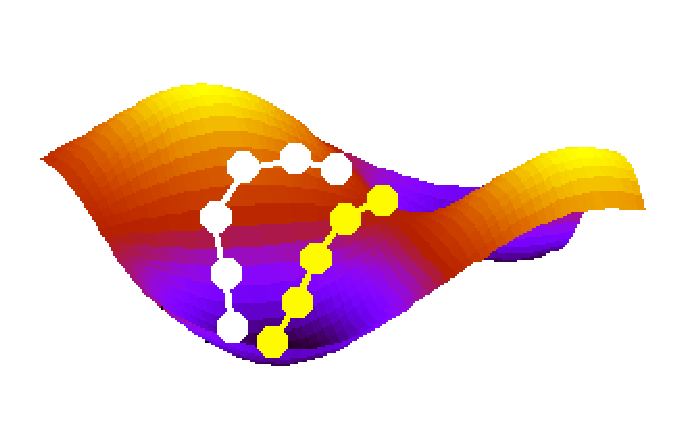
\includegraphics[scale=0.4]{surface_string.eps}
\caption{{\scriptsize  Free energy surface. }}
\end{figure}
}%
{
%Third quadrant
The free energy along the string is computed by~{\scriptsize PRB, {\bf 66}, 052301 (2002)},
\begin{equation*}
        F(z(\alpha)) - F(z(0))= \int^{\alpha}_0 \sum^N_{i=1} \frac{dz_i(\alpha')}{d\alpha'}
        \frac{\partial F(z(\alpha'))}{\partial z_i} d\alpha'
\end{equation*}
}%
{
%Fourth quadrant
%\begin{figure}
%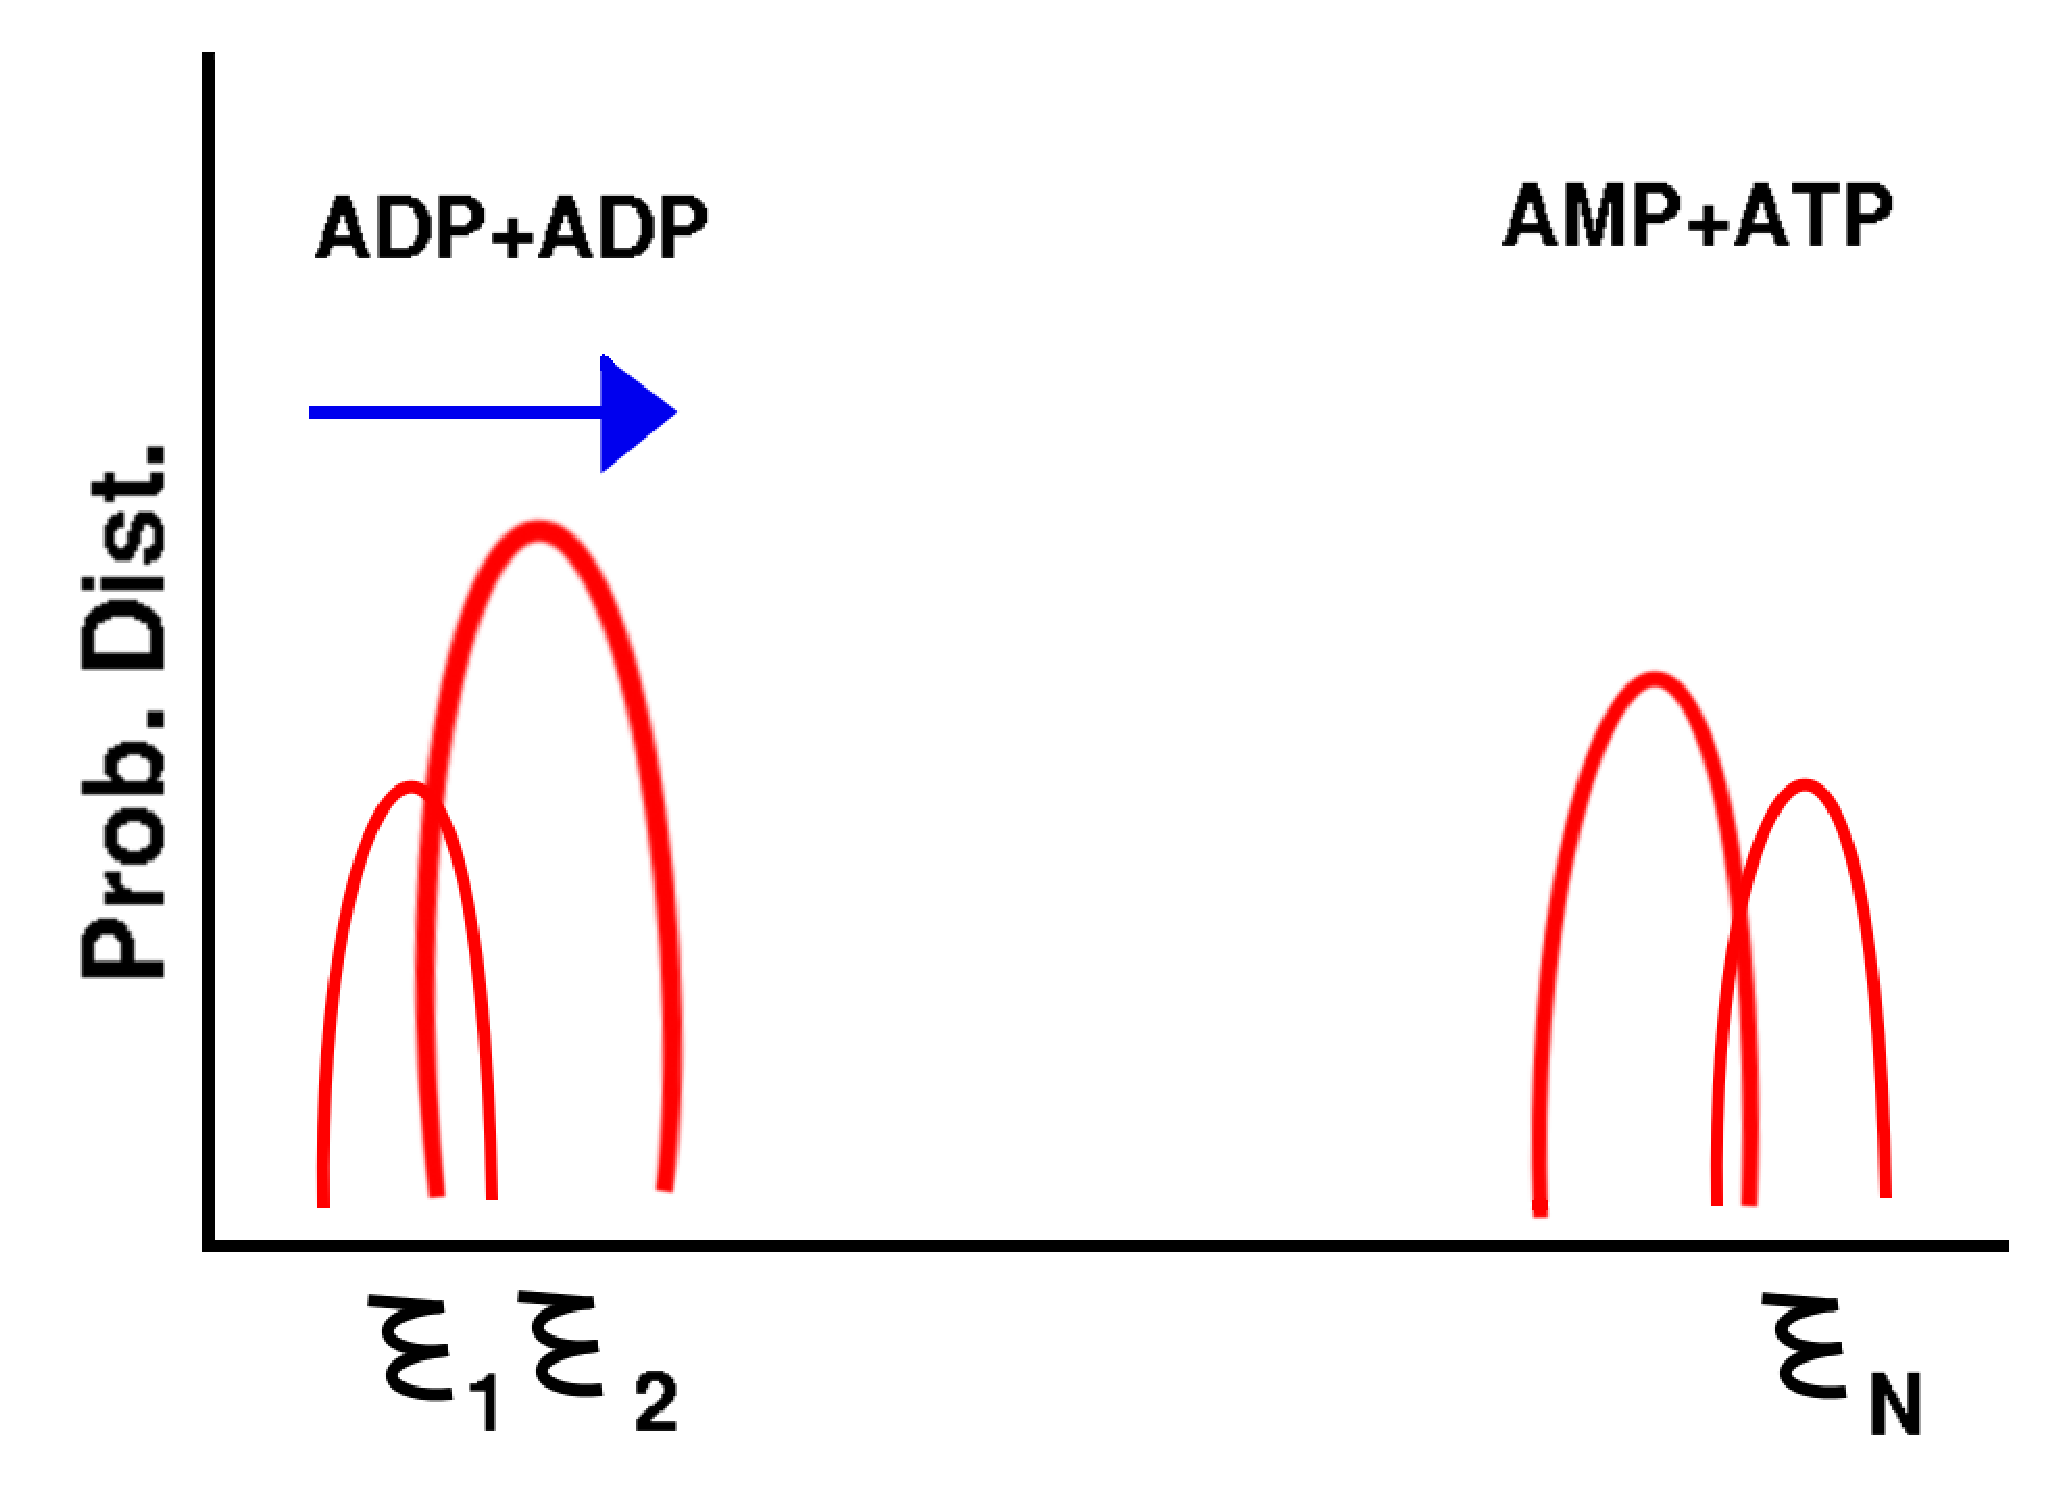
\includegraphics[scale=0.1]{prob_dist.eps}
%\caption{{\scriptsize  Probability histograms. }}
%\end{figure}
}
\end{frame}


\begin{frame}
\frametitle{String method (SM) simulations}
\begin{figure}
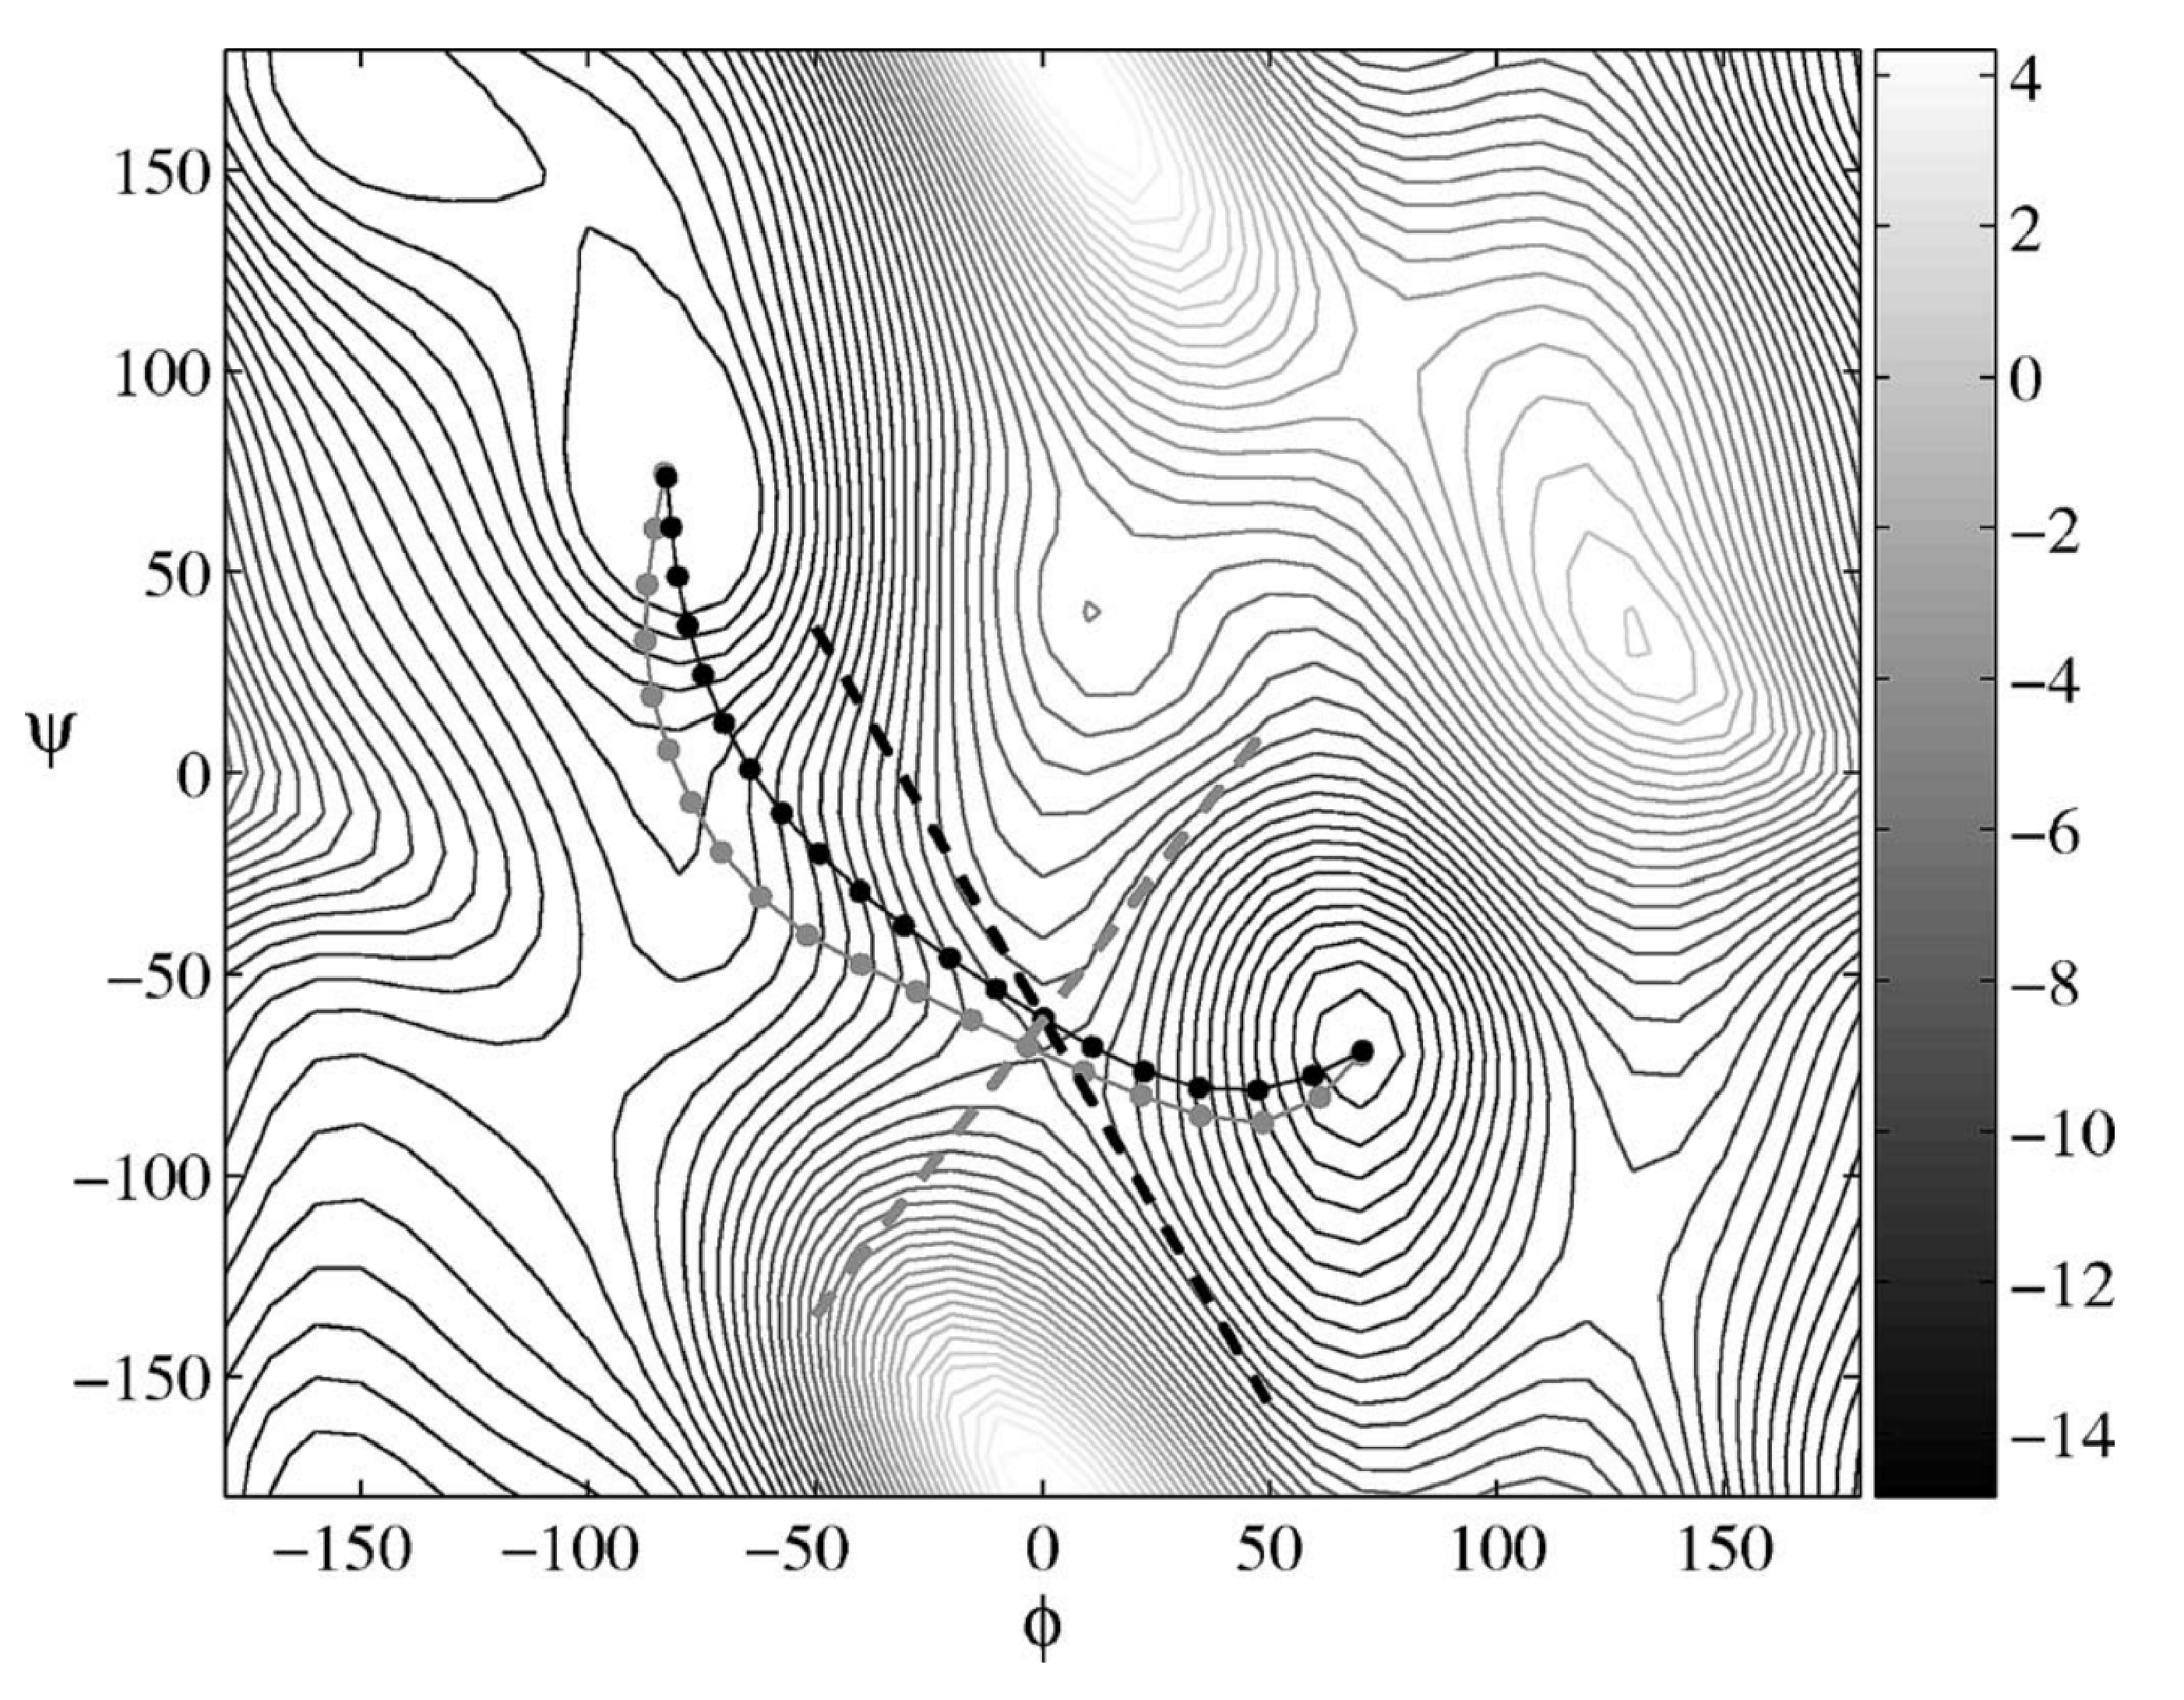
\includegraphics[scale=0.15]{string_fe.eps}
\caption{{\scriptsize  Free energy surface of Alanine dipeptide. }}
\end{figure}
\end{frame}


\subsubsection{Coarse graining} 


\begin{frame}
\frametitle{Coarse-grain simulations}
\begin{figure}
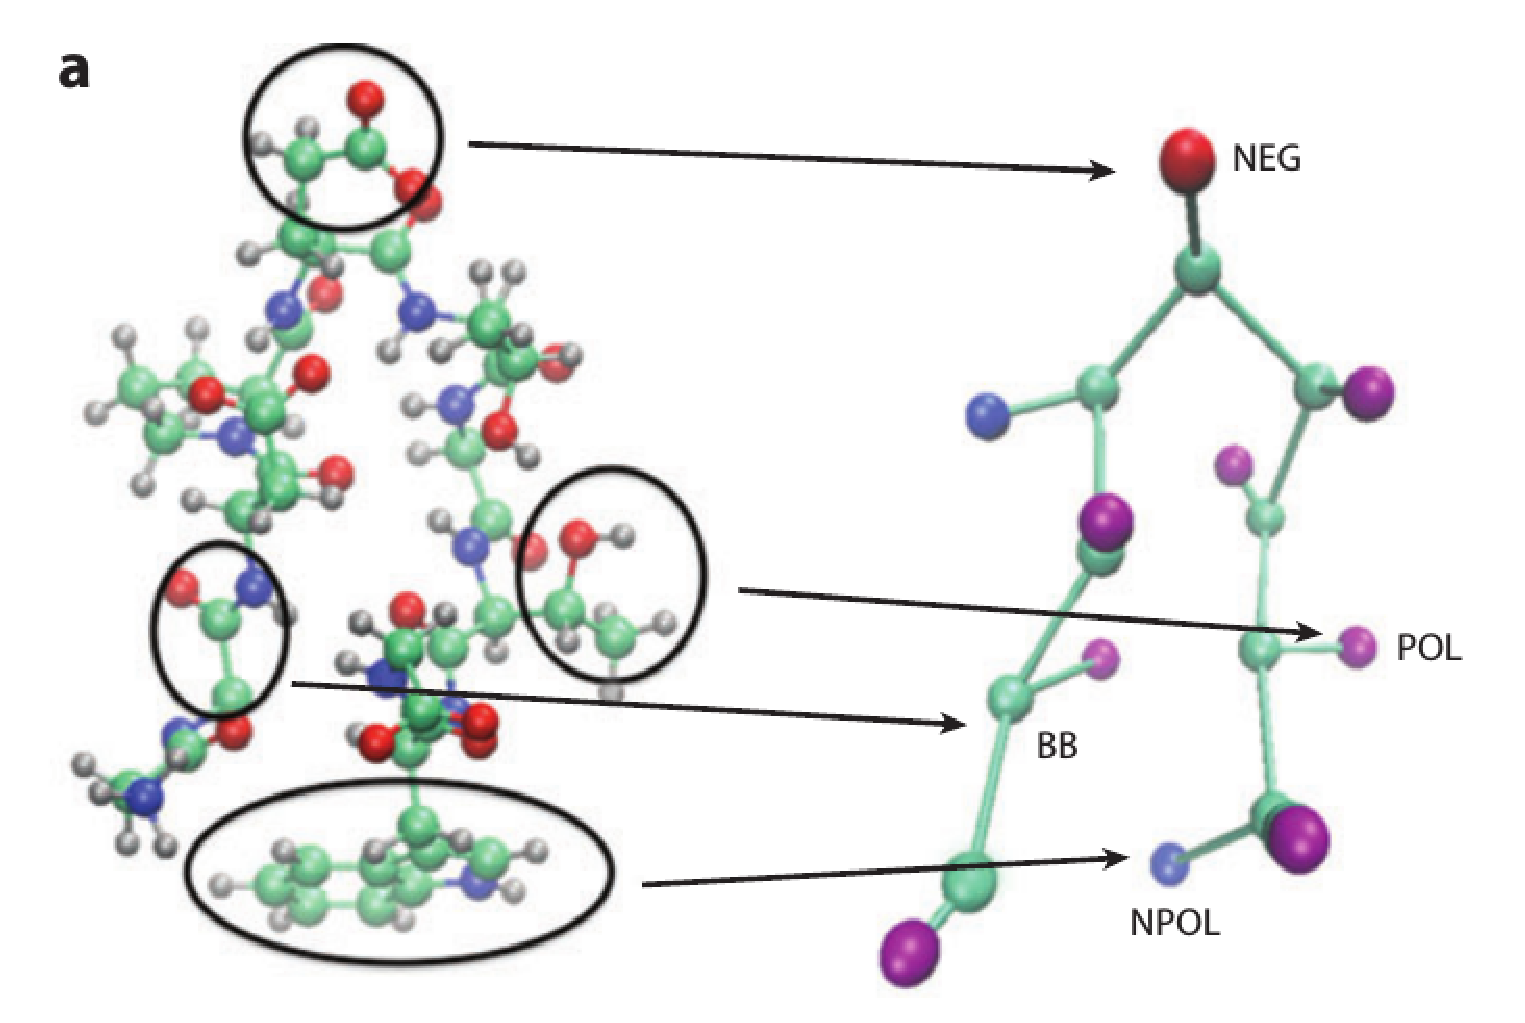
\includegraphics[scale=0.3]{coarse-grain.eps}
\caption{{\scriptsize  Reduction of the degrees of freedom [Annu. Rev. Biophys., {\bf 42}, 73 (2013)]. }}
\end{figure}
\end{frame}

\begin{frame}
\frametitle{Coarse-grain simulations}
\begin{figure}
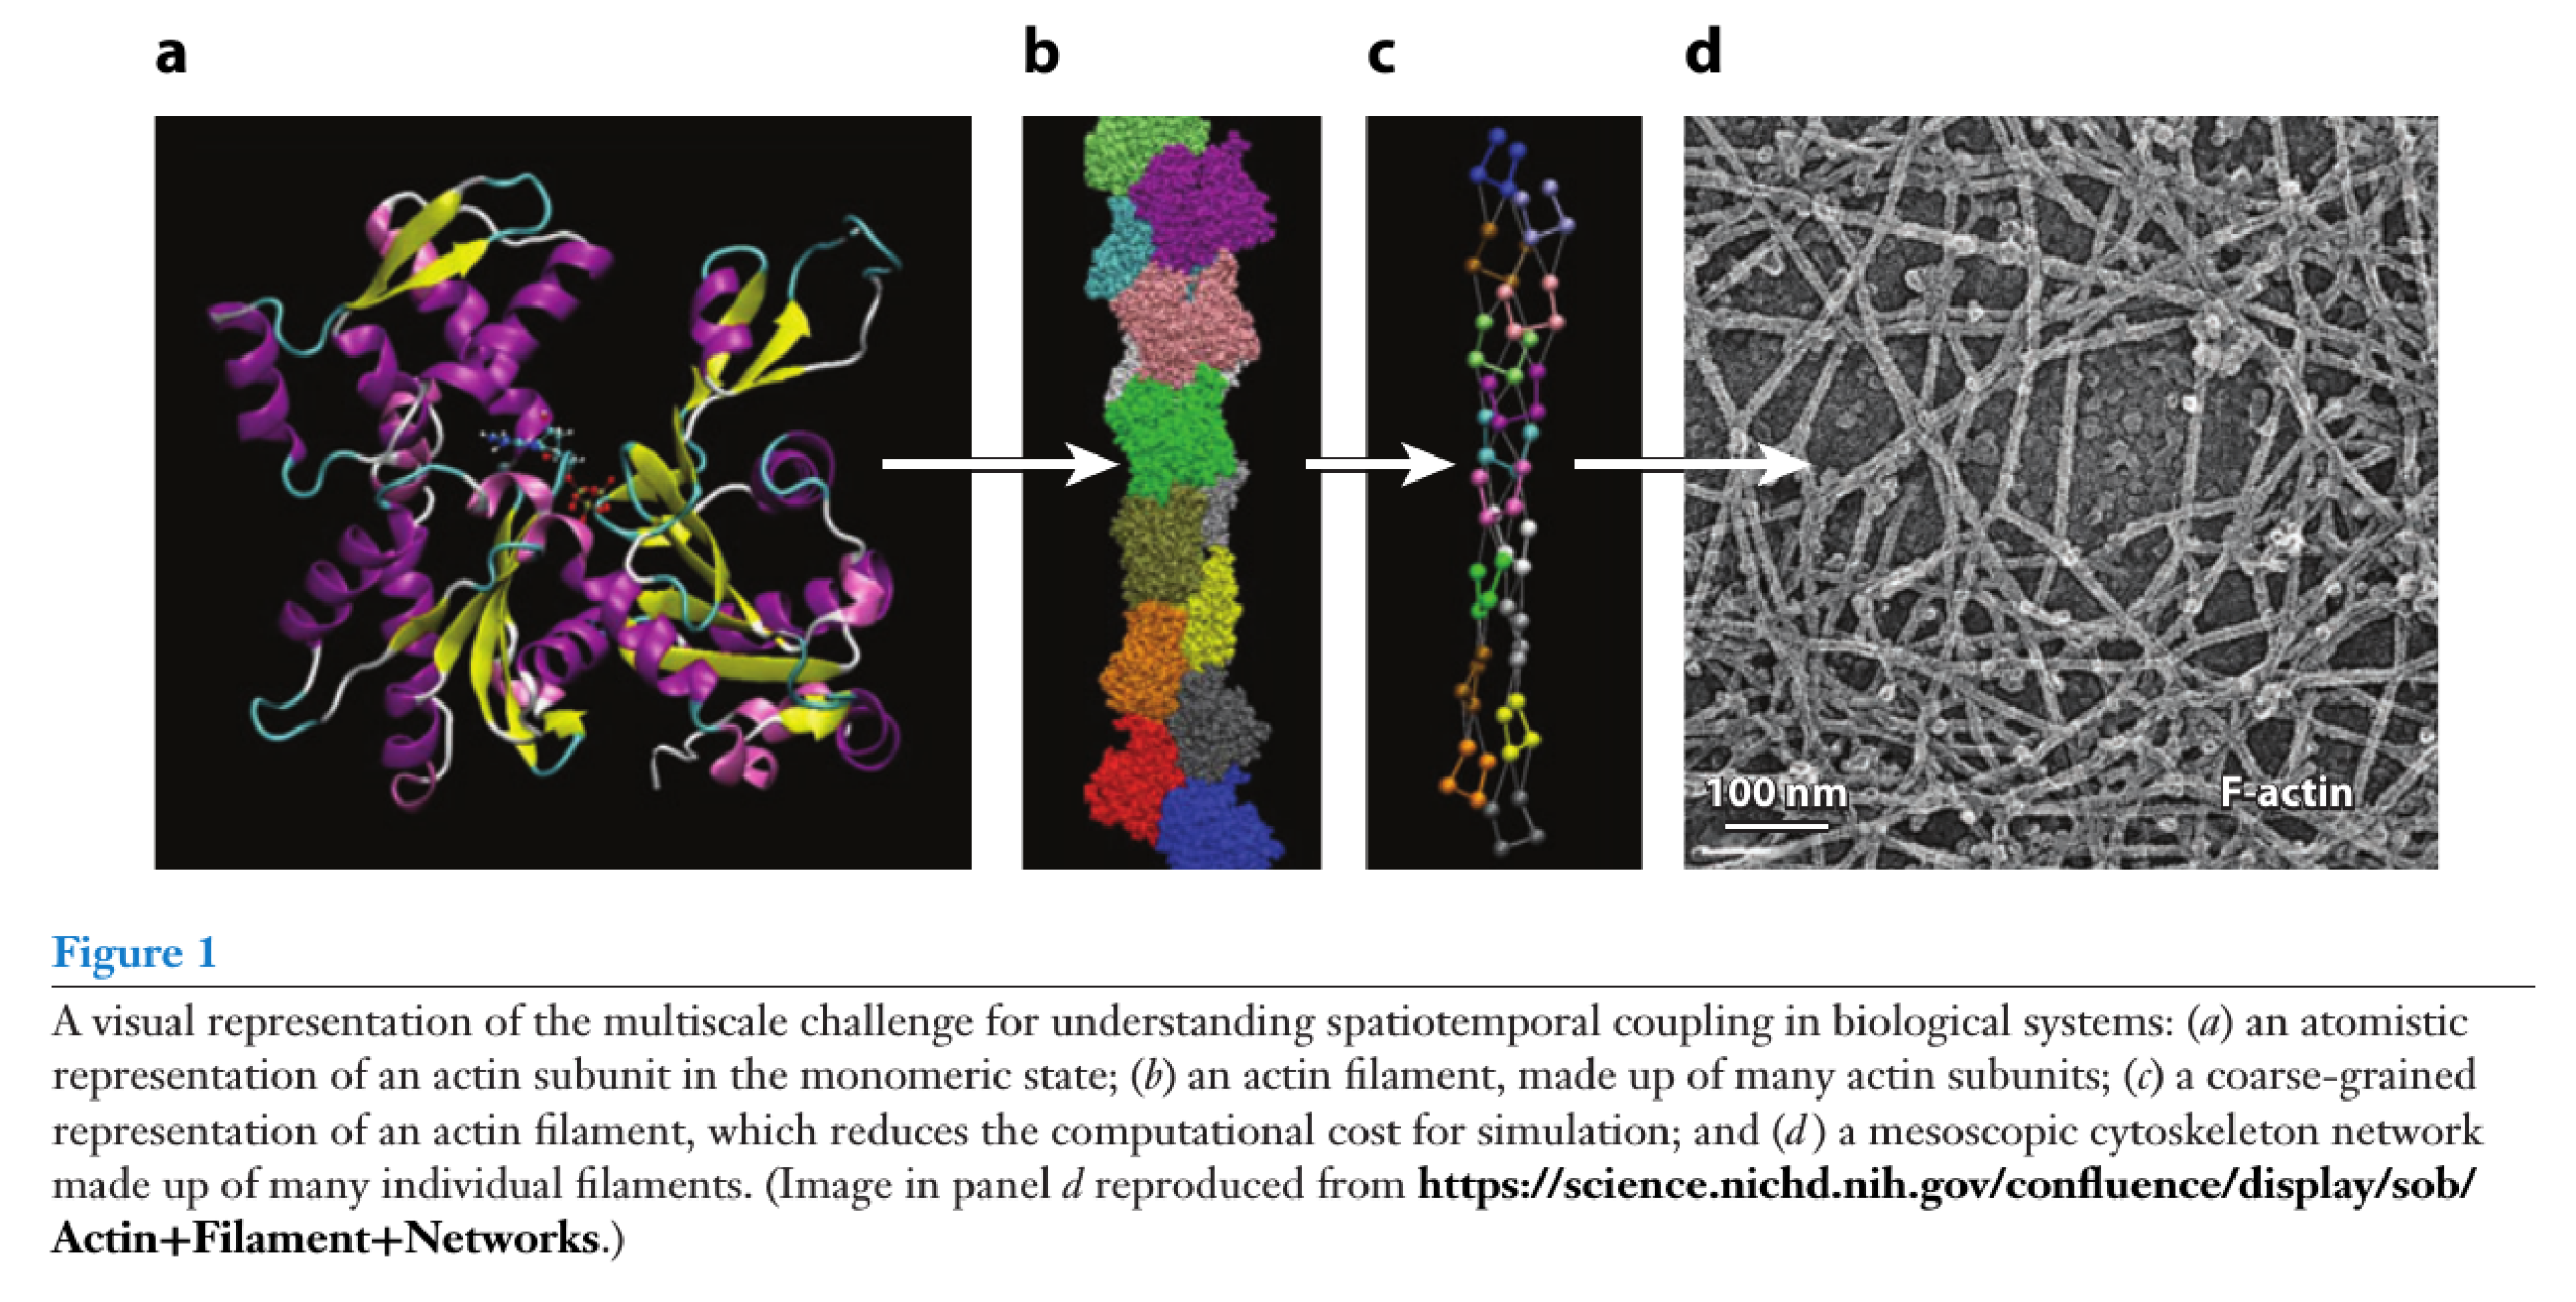
\includegraphics[scale=0.23]{coarse-grain-meso.eps}
\caption{{\scriptsize  Reduction of the degrees of freedom [Annu. Rev. Biophys., {\bf 42}, 73 (2013)]. }}
\end{figure}
\end{frame}



\subsubsection{Alchemical method} 


\begin{frame}
\frametitle{Alchemical simulations}


\begin{figure}
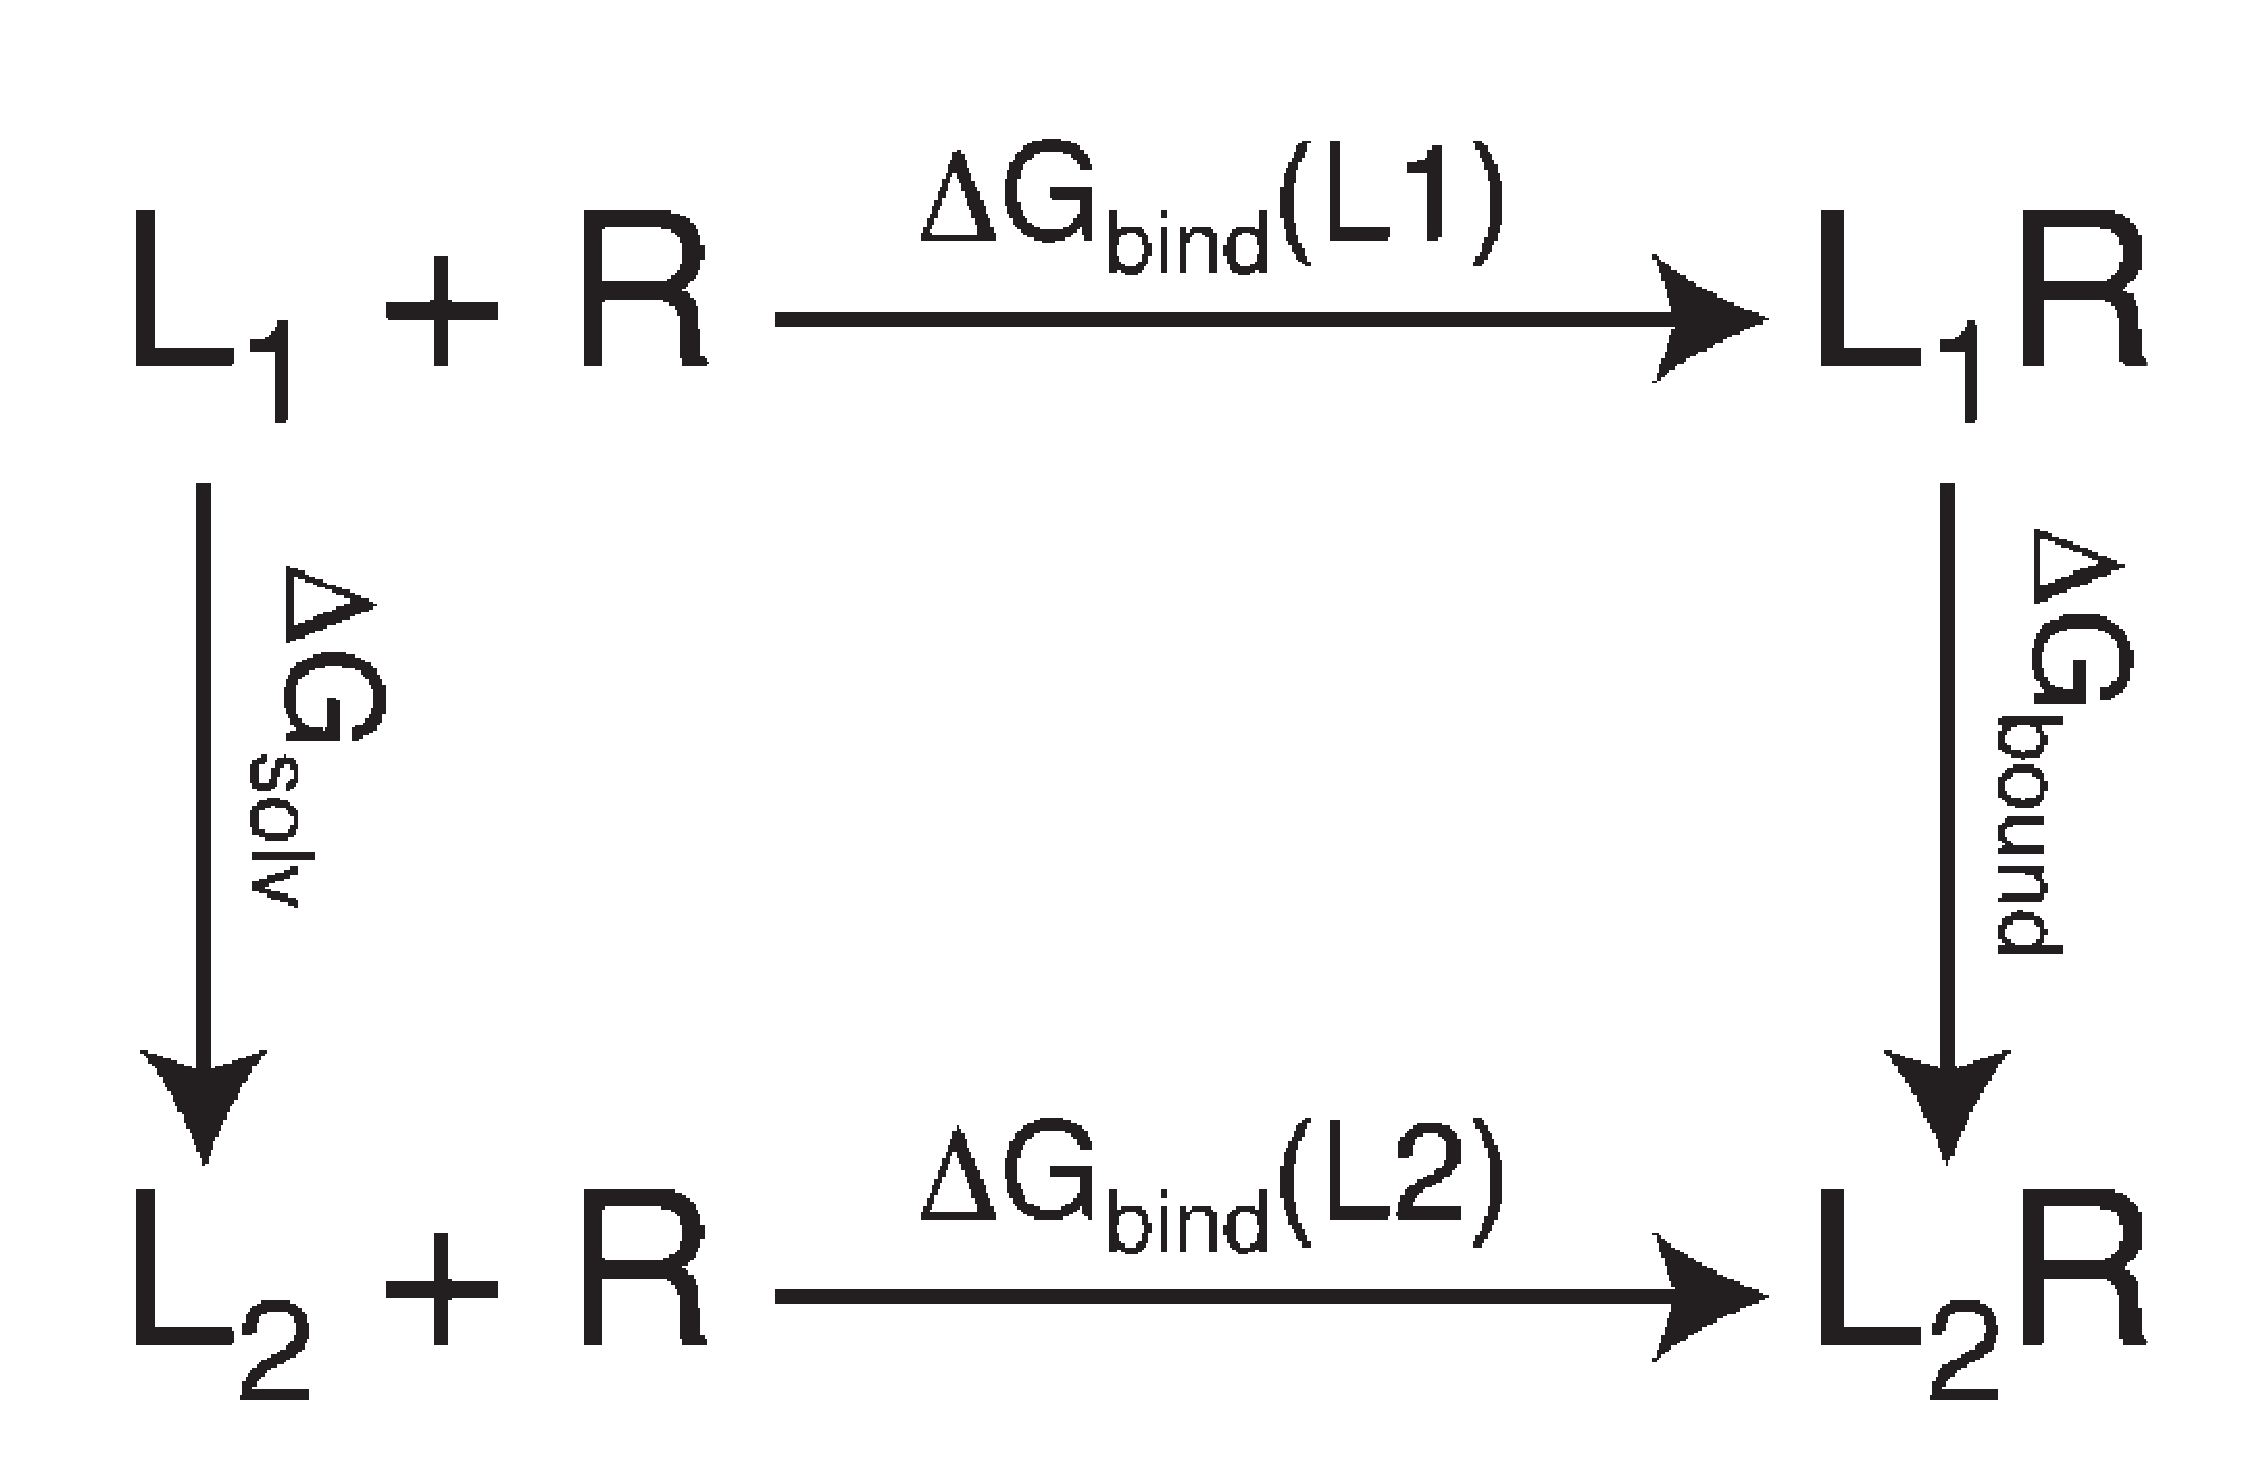
\includegraphics[scale=0.08]{alchemical.eps}
\caption{{\scriptsize  Thermodynamic cycle for binding of two protein ligands $L_1$ and $L_2$,
[JCC, {\bf 30}, 1692 (2009)]. }}
\end{figure}

\begin{equation}                                                                                                                                            
\label{Eq:ipspot}          
\Delta \Delta G_{L_i \rightarrow L_j}^{bind}=  \Delta G_{L_j}^{bind}-\Delta G_{L_i}^{bind}
= \Delta G_{RL_i \rightarrow RL_j}^{prot}- \Delta G_{L_i \rightarrow L_j}^{solv}
\end{equation}

The Hamiltonian is modified according to,

\begin{equation}                                                                                                                                            
	H=T_x + (1-\lambda)V_0 + \lambda V_1
\end{equation}



\end{frame}

\begin{frame}
\frametitle{Alchemical simulations}


\begin{figure}
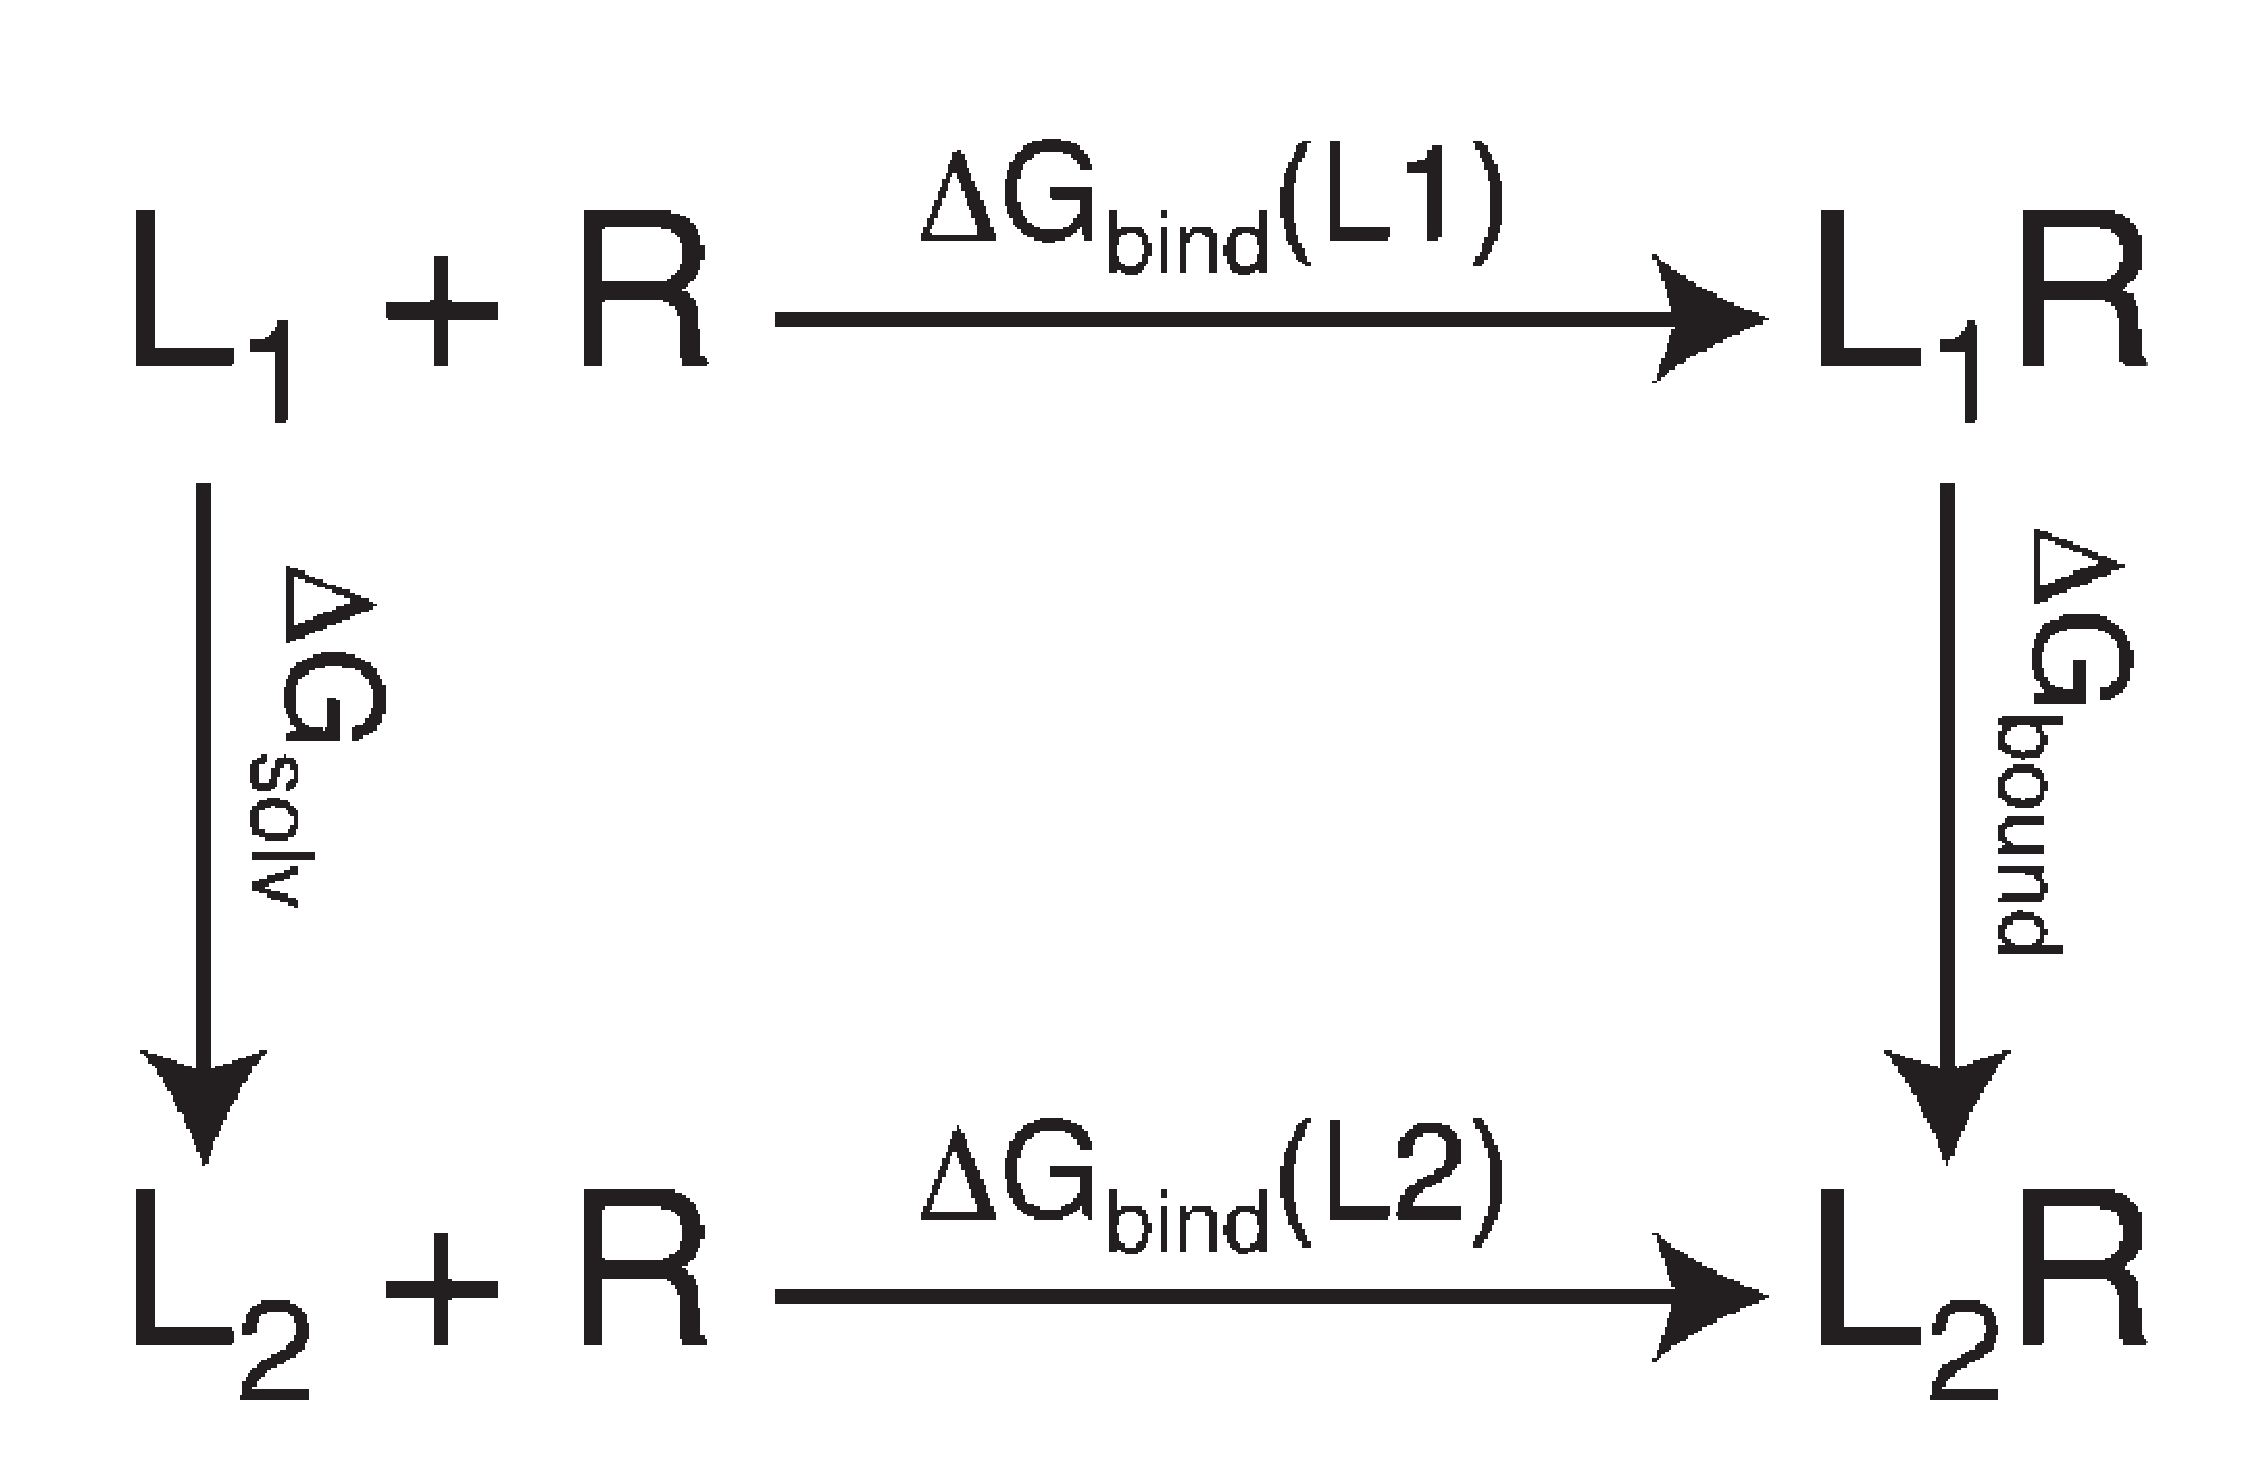
\includegraphics[scale=0.08]{alchemical.eps}
\caption{{\scriptsize  Thermodynamic cycle for binding of two protein ligands $L_1$ and $L_2$,
[JCC, {\bf 30}, 1692 (2009)]. }}
\end{figure}

The free energy difference going from $\lambda=0$ to $\lambda=1$ is,


\begin{equation}                                                                                                                                            
	\Delta G _{\lambda=0 \rightarrow \lambda=1 } = \sum_{\lambda=0}^{1} -\frac{1}{\beta}
	\ln \left< \exp \left( -\beta (H_{(\lambda+\delta \lambda)} - H_{(\lambda)}   )   \right) \right>
\end{equation}

\end{frame}

%%%%%%%%%%%%%%%%%% NEW  SLDE
%\section{Kebnekeise}
%\begin{frame}\frametitle{Abisko and Intro to Kebnekeise}
%
%	Birgitte Brydsoe
% 
%\end{frame}

\section{Using CHARMM at HPC2N}

%%%%%%%%%%%%%%%%% NEW  SLDE
\begin{frame}[fragile]
\frametitle{Installing CHARMM on Kebnekaise}


\begin{verbatim} 
Load the modules 
module load GCC/5.4.0-2.26  OpenMPI/1.10.3

go to the charmm folder and type:
./install.com gnu M

at the end of the installation one gets the message:
 install.com> CHARMM Installation is completed.
               The CHARMM executable is /pfs/nobackup/home/u/username/CHARMM_tutorial/charmm/exec/gnu_M/charmm.
\end{verbatim} 

\end{frame}

%%%%%%%%%%%%%%%%% NEW  SLDE
\begin{frame}[fragile]
\frametitle{Running CHARMM on Kebnekaise}

\begin{verbatim} 
#!/bin/bash
#SBATCH -A project-ID
#SBATCH -N 1
#SBATCH --time=01:00:00
#SBATCH --output=job_str.out
#SBATCH --error=job_str.err
#SBATCH --exclusive
#SBATCH --mail-type=END

module load GCC/5.4.0-2.26  OpenMPI/1.10.3

mpirun -np 28 /home/u/user/pfs/CHARMM_tutorial/charmm/exec/gnu_M/charmm \
 -i step4_equilibration.inp > out_equilibration.dat
mpirun -np 28 /home/u/user/pfs/CHARMM_tutorial/charmm/exec/gnu_M/charmm \
 cnt=1 -i step5_production.inp > out_production.dat
\end{verbatim} 

\end{frame}
\subsection{Setting up the system, minimization, solvation, equilibration, production and analysis.}

%%%%%%%%%%%%%%%%% NEW  SLDE

%%%%%%%%%%%%%%%%% NEW  SLDE
\begin{frame}
\frametitle{CHARMM}

\begin{itemize}
\item Setting up the system
\item minimization
\item solvation
\item neutralization
\item equilibration
\item production 
\item analysis
\end{itemize}

\end{frame}

%%%%%%%%%%%%%%%%% NEW  SLDE
\begin{frame}
\frametitle{CHARMM files}
\begin{itemize}
	\item *.pdb (coordinates)
	\item CHARMM parameter files 
	\item *.inp (input file for simulation)
\end{itemize}
\end{frame}

%%%%%%%%%%%%%%%%% NEW  SLDE
\begin{frame}
  \frametitle{Performance of CHARMM}

\begin{minipage}[t]{0.48\linewidth}

\begin{figure}
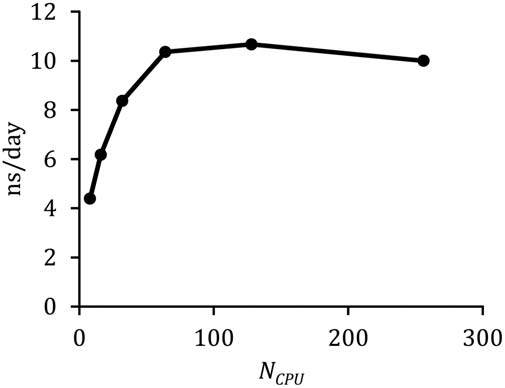
\includegraphics[scale=0.25]{pekka-charmm1.png}
\caption{{\scriptsize  Old CHARMM version.}}
\end{figure}

\end{minipage}
%}%
\hfill%
%\fbox{%
\begin{minipage}[t]{0.48\linewidth}
\begin{figure}
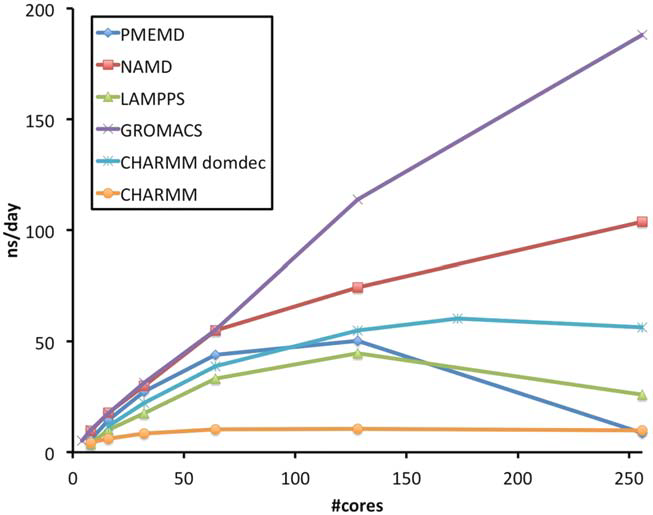
\includegraphics[scale=0.21]{pekka-charmm2.png}
\caption{{\scriptsize Comparison of CHARMM with other novel software.}}

\end{figure}
\end{minipage}

System of 19,609 atoms. JCC, {\bf 35}, 406-413 (2014)

\end{frame}

%%%%%%%%%%%%%%%%% NEW  SLDE
\begin{frame}
\frametitle{CHARMM support}
\begin{itemize}
	\item https://www.charmm.org/ubbthreads/
	\item contact HPC2N support
\end{itemize}
\end{frame}



\end{document}
